\documentclass[12pt,oneside]{article}

%%%%%%%%%%%%%%%%%%%%%%%%%%%%
%%   Zusaetzliche Pakete  %%
%%%%%%%%%%%%%%%%%%%%%%%%%%%%
\usepackage{acronym}
\usepackage{enumerate}
\usepackage{a4wide}
\usepackage{fancyhdr}
\usepackage{graphicx}
\usepackage{palatino}
\usepackage{blindtext}
\usepackage{multirow}
\usepackage[ruled,longend]{algorithm2e}
\usepackage{float}
\usepackage{amsmath}
\usepackage{amssymb}


%folgende Zeile auskommentieren für englische Arbeiten
%\usepackage[ngerman]{babel}

\usepackage[bookmarks]{hyperref}
\usepackage[T1]{fontenc}
\usepackage[utf8]{inputenc}
\usepackage[a-1b]{pdfx}
\usepackage[justification=centering]{caption}
%\usepackage[style=unsrt,natbib=true,backend=biber]{biblatex}
\usepackage{csquotes}
\usepackage{url}

\usepackage{minted}
\usepackage{multicol}
\usepackage{mdframed}
\usepackage[most]{tcolorbox}
\usepackage[T1]{fontenc}
\usepackage{tabu}
\usepackage{tabularx}
\usepackage{color}
\usepackage{colortbl}
\usepackage{xcolor}
\usepackage{subfig}
\usepackage{graphicx}
\newsavebox{\measurebox}
%%%%%%%%%%%%%%%%%%%%%%%%%%%%%%
%% Definition der Kopfzeile %%
%%%%%%%%%%%%%%%%%%%%%%%%%%%%%%

\pagestyle{fancy}
\fancyhf{}
\cfoot{\thepage}
\setlength{\headheight}{16pt}

%%%%%%%%%%%%%%%%%%%%%%%%%%%%%%%%%%%%%%%%%%%%%%%%%%%%%
%%  Definition des Deckblattes und der Titelseite  %%
%%%%%%%%%%%%%%%%%%%%%%%%%%%%%%%%%%%%%%%%%%%%%%%%%%%%%

\newcommand{\HSFTitle}[8]{

  \thispagestyle{empty}
\begin{center}
    
\includegraphics[width=0.8\textwidth]{logo.eps} \\
    \vspace*{\stretch{1}}
    \end{center}

  %\vspace*{\stretch{1}}
  {\parindent0cm
  \rule{\linewidth}{.7ex}}
  \begin{center}
    \vspace*{\stretch{1}}
    \sffamily\bfseries\Huge
    #1\\
    \vspace*{\stretch{1}}
    \sffamily\bfseries\large
    #3
    \vspace*{\stretch{1}}
  \end{center}
  \rule{\linewidth}{.7ex}

  \vspace*{\stretch{2}}
  \begin{center}
    %\Large #2 am #5 der HAW Fulda \\
    \Large #5 \\
    \vspace*{\stretch{1}}

    \large Matriculation No:  #4 \\[1mm]
    \large Supervisor:  #7 \\[1mm]
    \large Co-Supervisor:  #8 \\[1mm]

    \vspace*{\stretch{1}}
    \large Submitted on #6
  \end{center}
}

%%%%%%%%%%%%%%%%%%%%%%%%%%%%
%%  Beginn des Dokuments  %%
%%%%%%%%%%%%%%%%%%%%%%%%%%%%

\begin{document}

  \HSFTitle
      {A study of reinforcement learning algorithms in simulated robotics scenarios }        % Titel der Arbeit
      {Masters Thesis} % Typ der Arbeit
      {Alejandro Pajares Chirre}          % Vor- und Nachname des Autors
      {1331534}
      {Masters Thesis submitted to the Faculty of AI at HS Fulda}  % Name des FBs
      {29.05.2023}        % Tag der Abgabe
      {Prof. Dr. Alexander Gepperth}     % Name des Erstgutachters
      {Prof. Dr. David James}    % Name des Zweitgutachters

  \clearpage

\lhead{}
\pagenumbering{Roman}
    \setcounter{page}{1}

%%%%%%%%%%%%%%%%%%%%%%%%%%%%
%%  Kurzzusammenfassung   %%
%%%%%%%%%%%%%%%%%%%%%%%%%%%%
\clearpage
%
\markboth{Abstract}{Abstract}
\section*{Abstract}

The world of robotics has seen significant advancements in recent years, and this is largely due to the integration of machine learning techniques. Robots are now able to learn from their surroundings, make decisions, and carry out tasks with minimal human intervention. 
Machine learning has enabled robots to interact with humans and perform tasks that were previously considered impossible. In particular, reinforcement learning (RL) is a type of machine learning that models how humans learn from sensory input and motor responses in response to rewards. RL is based on the idea that an agent interacts with an environment by taking actions and receiving feedback in the form of rewards or punishments. Q-learning is a popular algorithm used in RL to learn the optimal policy, i.e., the best sequence of actions to maximize reward, for an agent. 
This thesis focuses on the application of reinforcement learning (RL) and Q-learning algorithms in controlling the motion of three joints of a six-degree-of-freedom (6-DOF) robotic arm in a simulated environment. To apply the Q-learning algorithms, the problem needs to be modeled as a Markov Decision Process, and during the learning process, the exploration and exploitation rate need to be balanced.
The robotic arm is modeled in Gazebo, and the control commands are sent using the Robot Operating System (ROS 2). The objective of the robotic arm is to touch the target. The RL algorithm learns to maximize the reward function, which is based on the current and previous distance between the target and one end of the robotic arm and the angles of the three joints being controlled. 
The experimental results demonstrate that RL and Q-learning algorithms can effectively control the motion of a robotic arm in a simulated environment. The robotic arm successfully learns to approach and touch the target.



% \par\noindent\rule{\textwidth}{0.4pt}

%The length of a thesis can vary depending on the subject. However, 50-55 pages for a master thesis is common, a little less for a bachelor thesis.
%Please pay careful attention to visual impression (sufficiently many and nicely made pictures/graphs, elegant formatting) as well as language (flawless English, elegant formulations), since these two points have are important for the grade. Furthermore, the introduction, discussion and conclusion chapters have a high impact on the grade, since people often read only those (which means they should be nice). 
\clearpage
\tableofcontents
\clearpage

\addcontentsline{toc}{section}{\listfigurename}
\listoffigures

\addcontentsline{toc}{section}{\listtablename}
\listoftables
\clearpage


%%%%%%%%%%%%%%%%%%%%%%%%%%%%
%%  Einstellungen  %%
%%%%%%%%%%%%%%%%%%%%%%%%%%%%
\cleardoublepage
\pagenumbering{arabic}
    \setcounter{page}{1}
\lhead{\nouppercase{\leftmark}}

%%%%%%%%%%%%%%%%%%%%%%%%%%%%
%%  Hauptteil  %%
%%%%%%%%%%%%%%%%%%%%%%%%%%%%

\section{Introduction} \label{sec:einleitung}

Designing, building, operating, and programming robots is the primary objective of the engineering and scientific discipline of robotics. A robot is a device created to carry out operations mechanically or somewhat autonomously, frequently imitating human actions or behavior \cite{1_o2019legal}. Numerous industries and applications, including agriculture, manufacturing, healthcare, transportation, entertainment, and the military, use robots. Robots are frequently utilized in industry to complete tasks like welding, creating art, integration, and packing that could be repetitious or dangerous for human workers. Robots are employed in agriculture to do duties including planting, harvesting, and crop monitoring \cite{2_roldan2018robots}. Robots are utilized in the transportation industry for logistics, warehouse management, and autonomous driving. Robots are employed in the entertainment industry for activities including animatronics as well as special effects. Robots are employed in the military for operations including bomb disposal, surveillance, and reconnaissance. Robots are evolving rapidly in terms of versatility, intelligence, and adaptability, as well as in terms of possible applications. Robotics is an emerging discipline that has the potential to significantly alter numerous aspects of our everyday lives and will probably become more crucial in determining our future \cite{3_bostrom2018ethics}.

Numerous companies have embraced the use of robotics to aid humans in tasks that are monotonous, physically demanding, or hazardous. Yet, acquiring a robot and hiring a robotic engineer to create a tailored solution for a particular task requires a significant investment of resources.
The duties of a robot engineer include setting up communication, designing control scripts, computing coordinate transformations, and creating error-handling programs. Typically, a technician takes on the task of operating the robot on a daily basis, or the robot operates on its own. However, if the task requirements or processes change, it is difficult to modify the existing robotic solution to suit a new configuration or application without the assistance of a robot engineer, despite the significant resources invested in acquiring and developing it.
Instead of relying on a robotic engineer to manually program a robot's operations for a new application, companies could employ deep reinforcement learning to train an intelligent agent to control the robot specifically for that application. This approach would enable the resources invested in robotics to be more adaptable and versatile, suitable for a broader range of applications and purposes.

This thesis is about reinforcement learning which is a type of machine learning that involves an agent learning from its interactions with an environment in order to maximize a reward signal over time \cite{suttonAndBarto}. It is a method of learning that involves trial and error, with the agent receiving feedback in the form of rewards or punishments for its actions. According to Kaelbling, Littman, and Moore \cite{kaelblingLittmanAndMoore}, reinforcement learning can be defined as "a problem faced by an agent that learns behavior through trial-and-error interactions with a dynamic environment".
Many different concepts and methodologies can be used to break down reinforcement learning. This work focuses on Deep Q learning, and to study it, a simulated robotic arm is trained to touch a can.

% Generally, the introduction should be VERY detailed, with a focus on pedagogical value. 10-15 pages are expected here! Everything that contributes to clarity (pictures, diagrams, ...) is allowed or even expected. The introduction is meant for people who DO NOT have a computer science degree, or even any particular affinity to computers, so focus on the "big picture".  
%
\subsection{Context}
%What is the context of the presented work? If you work in a company, present the company first. Then the broad scientific or technological background in which the work is embedded should be presented and explained.
\subsubsection{Simulated Robotics} 
Simulated robotics is a rapidly developing field of study that strives to create intelligent systems that can communicate with virtual worlds in a manner that is comparable to how actual robots communicate with the real world \cite{4_choi2021use}. Compared to traditional robots, simulated robotics has many benefits, such as lower costs, more flexibility, and the ability to test and improve algorithms in a secure setting. Simulated robotic systems can be applied to a variety of tasks, from straightforward ones like object detection and manipulation to more difficult ones including autonomous navigation, group decision-making, and experience-based learning.  
\begin{figure}[H]
\centering
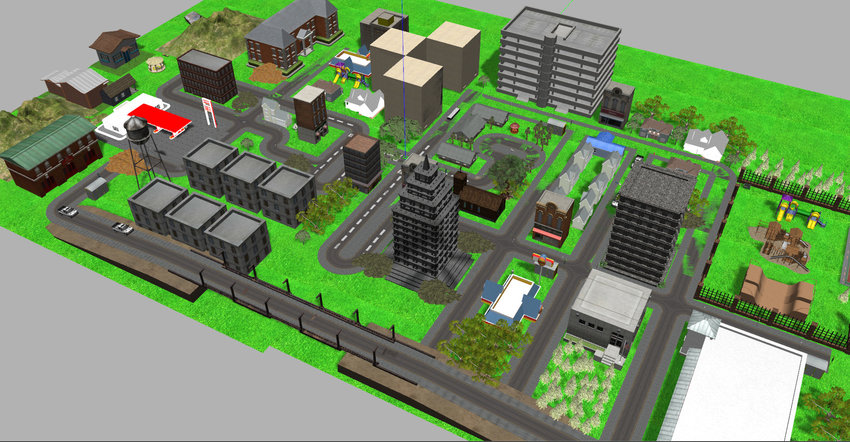
\includegraphics[width=0.9\linewidth]{gazebo_city}
\caption{Simulated urban scenario created in Gazebo \cite{yigit2020real}.}
\label{fig:gazebocity}
\end{figure}

The application of virtual environments for autonomous vehicle training and testing is an illustration of simulated robotics \cite{5_elmquist2021sensor}. To train and test the computer programs that operate autonomous vehicles, researchers can develop realistic simulations of numerous driving circumstances and scenarios, like traffic patterns, atmospheric conditions, and unforeseen incidents. With this strategy, researchers may evaluate the dependability and safety of autonomous vehicles in a safe setting before placing them on public roads. The application of virtual environments to train and test robots for search and rescue missions is another illustration of simulated robotics \cite{6_sampedro2019fully}. In order to train and test robotics that can aid in rescue operations, researchers can develop simulations of emergencies such as earthquakes or floods. With this method, researchers may test the efficacy and security of various robotic systems and algorithms in a range of circumstances without endangering human responders.
Systems for industrial automation can also be developed using simulated robotics. For instance, manufacturers can build and test robotic assembly lines, improve production workflows, and spot possible bottlenecks or safety risks using simulations. Before installing physical systems in the real world, this method enables manufacturers to optimize their procedures and increase productivity.

\subsubsection{Industrial Automation}
Automation of industrial processes, such as manufacturing and construction, via the use of technological devices and control systems is known as industrial automation \cite{7_leitao2016industrial}. Industrial automation can be accomplished utilizing simulated robotic arms to carry out operations that would typically be carried out by human workers or actual robots. This entails creating the algorithms and control frameworks necessary for the virtual robotic arm to move and handle items precisely and effectively, as well as incorporating the virtual arm into a larger system that is capable of carrying out difficult tasks on its own.
Applications for simulated robotic arms in industrial automation include material handling, manufacturing work, quality control examinations, and machine maintaining. Companies can decrease the expenses of real robots and human labor while boosting production and efficiency by deploying virtual robotic arms \cite{8_javaid2021substantial}. Additionally, for increased flexibility and scalability, simulated robotic arms can be flexibly customized and adapted to various industrial environments. All things considered, the employment of simulated automated arms for automation in industry is a promising area of study and development, with tremendous potential for enhancing industrial procedures and developing the field of robotics.

\begin{figure}[H]
\centering
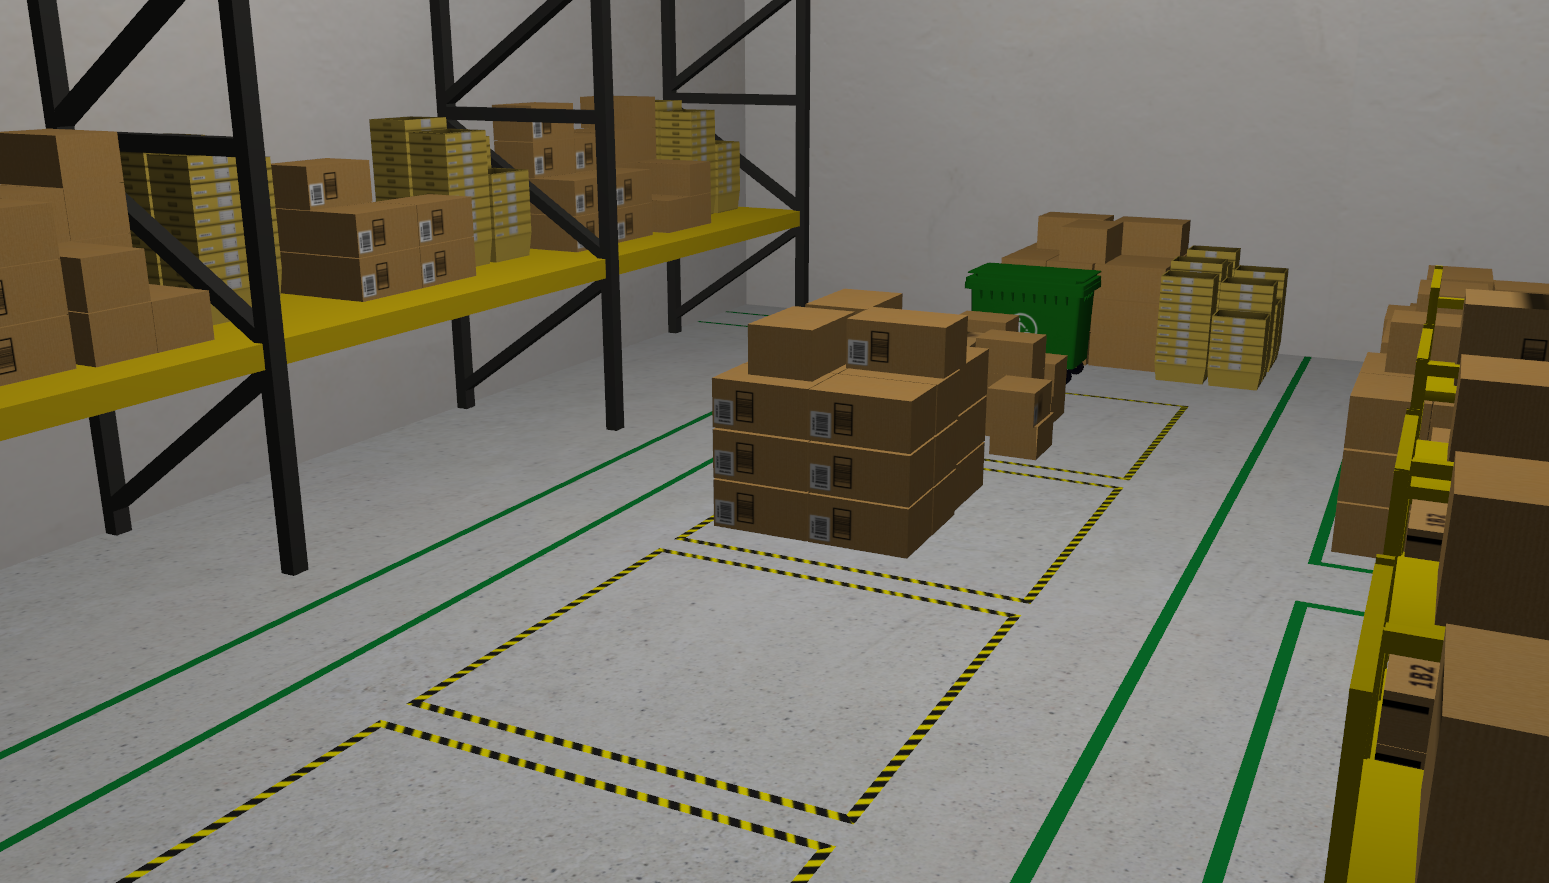
\includegraphics[width=0.9\linewidth]{gazebo_city1}
\caption{Small Warehouse Gazebo simulation \cite{aws-robomaker-small-warehouse-world}.}
\label{fig:gazebocity1}
\end{figure}


\subsubsection{Robotic Arms}
Traditionally developed industrial robots have been confined to closed cells or limited-access warehouse areas \cite{9_lucchi2020robo}. They typically perform repetitive operations on standardized objects without human interaction. Programming these robots is usually a time-consuming process that requires specialized knowledge of the machine's software. However, current trends in robotics aim to make robots capable of operating in dynamic and open environments where they can work alongside humans. This presents new challenges that require equipping the robot with sensors to perceive its surroundings and interact with objects. However, integrating and utilizing sensor data for planning the robot's actions is not an easy task.
A robotic arm functions like a human arm and is a mechanical system that typically includes an end effector for manipulating and interacting with the environment \cite{10_ohta2018design}. Robotic arms have various applications in industrial and service fields, such as pick and place, exploration, manufacturing, laboratory research, and space exploration. An arm with 6 degrees of freedom can pivot in six different directions, similar to a human arm. In industrial robotic arms, the mechanical structure and control mechanism are major factors of concern.
\begin{figure}[H]
\centering
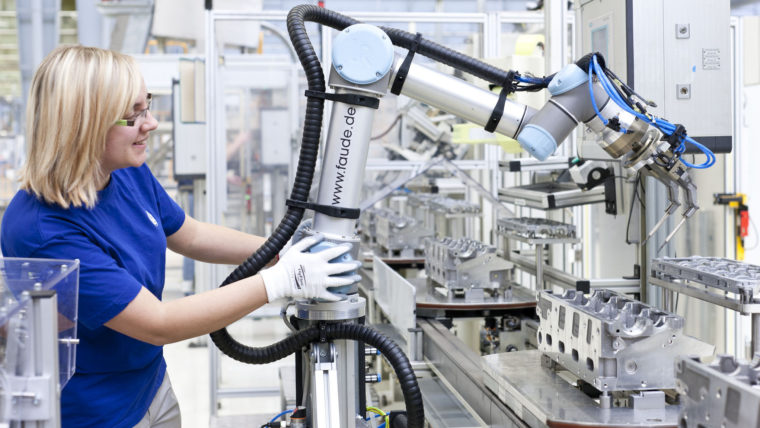
\includegraphics[width=0.9\linewidth]{robotic_arm_real_world}
\caption{A robot arm helps make engine components at a Volkswagen factory in Germany \cite{wamu2013}}
\label{fig:roboticarmrealworld}
\end{figure}
These arms are commonly used in a variety of applications, such as manufacturing, assembly, material handling, and surgery. Robotic arms can be controlled by various means, including joystick or slider controls, keyboard-based interfaces, and programmed motions. They can be programmed to perform repetitive tasks with high precision and speed, which makes them ideal for use in industrial settings where consistency and efficiency are crucial. These arms can be equipped with various end effectors, such as grippers, cameras, or welding tools, depending on the specific task that needs to be performed. They can also be designed to have multiple joints or degrees of freedom, which enables them to move in a wide range of directions and perform complex tasks. Advancements in robotics technology have led to the development of lightweight and portable robotic arms that can be easily integrated into various systems \cite{11_singh2013evolution}. These arms are becoming increasingly popular in areas such as healthcare and rehabilitation, where they can assist with tasks such as lifting and moving patients.

The primary focus of current research efforts is on training the robot’s arm to carry out various tasks autonomously using deep learning technologies. However, due to the massive amount of data required to teach a robot effectively, a data-driven approach is necessary. This can be challenging to achieve using a physical robotic arm. Therefore, developers have turned to robot simulation software \cite{12_oRobotics}, \cite{13_pybullet} to overcome the limitations of data-intensive AI approaches and to provide a stable environment \cite{14_banks1999introduction}. In a simulated environment, it is possible to control every aspect of the world, including impractical factors in reality. Moreover, there is no risk of damaging robots or human operators in simulations, and time control allows for faster data collection.

\subsubsection{Robot Operating System (ROS) and Gazebo}
The Robot Operating System (ROS) is a set of software libraries and tools that enables developers to build robotic applications \cite{15_quigley2009ros}. It provides a framework for writing and running code across multiple computers and devices, making it easier to create complex robotic systems. ROS was first developed in 2007 by Willow Garage, at robotics research lab \cite{16_cousins2014willow}. Since then, it has become widely adopted by the robotics community and is now supported by the Open Robotics organization. It offers a comprehensive platform for managing robotic systems. Originally designed to facilitate research in robotics, ROS is a unique framework. To grasp the fundamentals of the ROS framework, it is essential to comprehend the concept of message communication between nodes using topics.
One of the key features of ROS is its ability to handle communication between different components of a robotic system, such as sensors, actuators, and controllers \cite{17_emmi2014new}. This communication is done using a publish-subscribe messaging system, which allows components to share data and commands in real-time. ROS also provides a wide range of tools and libraries for tasks such as perception, navigation, and manipulation, which can be used to build complex robotic applications. These tools include algorithms for object recognition, path planning, and motion control, among others. Another advantage of ROS is its open-source nature, which means that developers can contribute to the development of the software and share their own code with the community. This has led to a large and active community of developers working on ROS, which has helped to drive its development and adoption.

Gazebo, on the other hand, is like a virtual playground for robots. It is a special computer program that lets you create a digital world where robots can move around and interact. It is like a video game, but instead of playing as a character, we get to control and test robots.
In Gazebo, we can build different environments like houses, parks, or even other planets. We can also design and customize our own robots with different shapes, sizes, and abilities. Once we have our world set up and our robots ready, we can make them move, perform tasks, and see how they interact with the surroundings.

Gazebo is useful because it allows us to experiment and learn about robotics without having to build and test everything in the real world. We can try out different robot designs, program them to do specific tasks, and see how they behave in different situations. It helps engineers and researchers save time and resources by simulating and testing their ideas virtually.

So, Gazebo is a computer program that lets us create worlds for robots to explore and learn in. It can be seen as a virtual playground where we can build robots and see how they work before bringing them to life in the real world.

\begin{figure}[H]
\centering
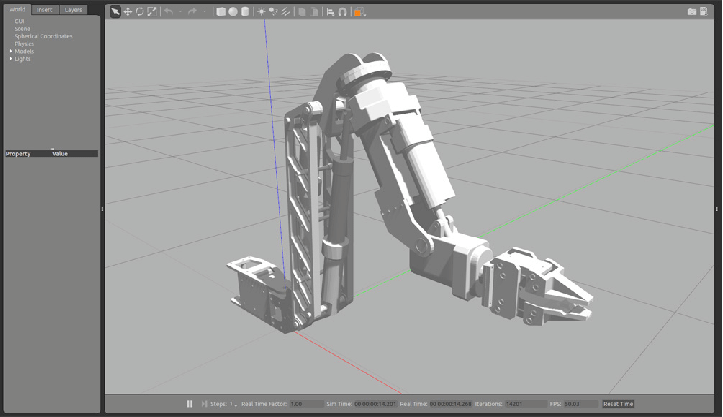
\includegraphics[width=0.9\linewidth]{gazebo_robotic_arm}
\caption{Gazebo simulation of a Robotic Arm in a Pick and Place setup. \cite{mathworks2021}.}
\label{fig:gazeboroboticarm}
\end{figure}

\subsubsection{Simulations}
Simulations serve as an entry point for Digital Twins, which are highly accurate depictions of the physical world \cite{19_lu2020digital}. These Twins can aid in boosting manufacturing output and improving the flexibility of supply chains. To streamline the implementation of manufacturing processes during production line changes, digital twinning involves linking simulation software to an actual self-governing robotic system. A robotic arm digital twin solution is showcased in a recent study \cite{20_tavares2018flexible}, where the authors employed ROS \cite{21_ros} to achieve smooth functioning between the virtual and real worlds. Simulating software has its limitations as it cannot accurately represent the real world due to the imperfections in their physics engines. 

Additionally, simulations have the advantage of providing perfect data with no interference, which has supported the exploration of deep learning approaches in robotics research.
Simulations are a powerful tool for designing and testing robotic arms. They allow engineers to create virtual models of robotic arms and simulate their behavior in different scenarios, without the need for a physical prototype. In a robotic arm simulation, the arm's mechanical structure, control system, and sensors are modeled in a virtual environment. The simulation can then be used to test the arm's performance in various tasks, such as picking and placing objects, assembling parts, or performing complex movements. One of the key benefits of using simulations for robotic arm design is that they can help identify potential issues or inefficiencies before a physical prototype is built \cite{22_browning2001applying}. This can save time and resources, as well as improve the overall design of the arm. Simulations can also be used to optimize the control system of a robotic arm. By simulating the arm's behavior in different scenarios, engineers can identify the optimal control strategy for achieving a specific task or movement. 

The ROS framework includes a useful tool called RViz, which enables us to observe the robot's pose or estimation in a 3D environment \cite{23_kulkarni2021visual}. With the correct configuration of the URDF file, the robot model can be visualized in RViz.  Furthermore, simulations can help train and test algorithms for robotic arm control, such as RL methods or deep learning approaches. This can be done by running simulations with different environments and scenarios and using the resulting data to train and refine the algorithms.

\subsubsection{Reinforcement Learning}
Reinforcement learning is like teaching a computer to make decisions and get better at them over time, similar to how we learn from our mistakes and improve. Consider the robotic arm in this thesis, we want to train it to perform a simple task which is touching an object. We do not give the robotic arm a list of instructions for every situation; instead, we want the robotic arm to learn on its own.

In reinforcement learning, the robot interacts with its environment. It takes actions, and based on those actions, it receives feedback in the form of rewards or punishments. Just like when humans do something good, they get a reward, and when they do something bad, they might get scolded.

The robot's goal is to figure out the best actions to take in different situations to maximize its rewards. It starts by trying random actions and seeing what happens. Over time, it learns from the feedback and adjusts its actions to get more rewards and fewer punishments. 
\begin{figure}[H]
  \centering
  \subfloat[Simulated robotic arm starting position.]{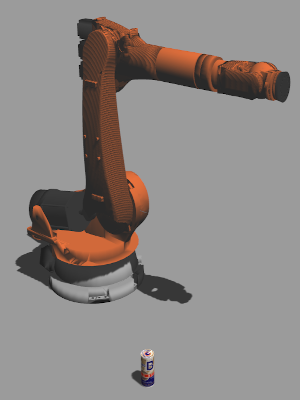
\includegraphics[width=0.4\textwidth]{intro_kuka01_n}\label{fig:intro_kuka01_n}}
  \subfloat[Simulated robotic arm moving away from the target object.]{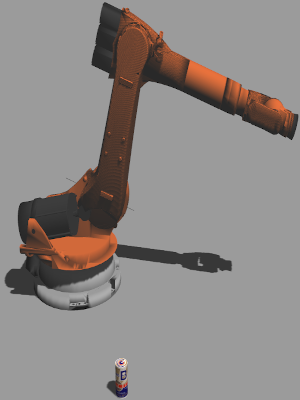
\includegraphics[width=0.4\textwidth]{intro_kuka02_n}\label{fig:intro_kuka02_n}}
  \\
  \subfloat[Simulated robotic arm starting position.]{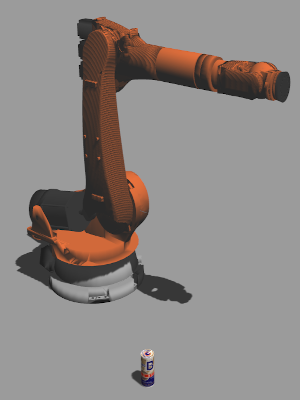
\includegraphics[width=0.4\textwidth]{intro_kuka01_n}\label{fig:intro_kuka0103_n}}
  \subfloat[Simulated robotic arm moving closer to the target object.]{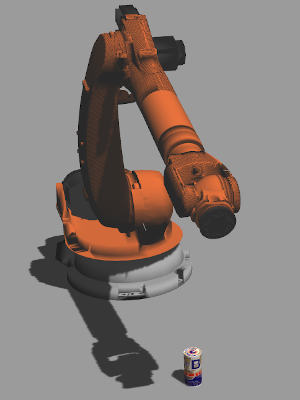
\includegraphics[width=0.4\textwidth]{intro_kuka03_n}\label{fig:intro_kuka03_n}}
  \caption{Robotic arm Kuka KR210 moving closer and away from the target.}
  \label{fig:intro_kuka}
\end{figure}
For example, in the process of trying random actions; in Figure \ref{fig:intro_kuka}, when the robotic arm moves from Figure \ref{fig:intro_kuka01_n} to Figure \ref{fig:intro_kuka02_n} it gets away from the target object so in this case the robotic arm is punished with a negative reward. On the other hand, when it moves from Figure \ref{fig:intro_kuka0103_n} to Figure \ref{fig:intro_kuka03_n} it gets closer to the target object, and therefore it receives a positive reward.
It can be seen as a game where the robotic arm is the player, the environment is the game world, and the rewards are the points it earns. The more points it earns, the better it gets at playing the game. 
In our example, consider Figure \ref{fig:introkuka04} when the robotic arm finally touches the target object it gets the highest possible reward and ends the game victoriously.
To help the robot learn, we use special algorithms that guide its decision-making instead of just random actions. These algorithms learn from the experiences and feedback, just like humans learn from our mistakes and successes.

\begin{figure}[H]
\centering
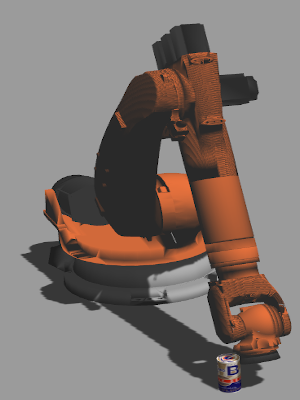
\includegraphics[width=0.35\linewidth]{intro_kuka04_n}
\caption{Simulated robotic arm touching the target object.}
\label{fig:introkuka04}
\end{figure}

Reinforcement learning is exciting because it allows machines to learn and adapt without us telling them exactly what to do. They explore, learn from their actions, and become better at solving problems. It is like watching our pet robot grow smarter and more capable over time.

\subsection{Problem Statement}

Many studies have demonstrated that utilizing reinforcement learning (RL) presented a viable solution for addressing the limitations of conventional methods in tackling intricate robotics tasks. Numerous AI experts have created various frameworks and toolkits to examine and assess their algorithms' effectiveness in solving challenging problems \cite{36_wu2020ethical}. Although the outcomes were remarkable, these applications were generally limited to simulated environments and seldom deployed in real-world scenarios. Numerous researchers are presently focused on a highly promising mission of bridging the gap between simulation and reality. However, proficiency in various domains is crucial in the intricate field of RL, which might be an obstacle to entry for roboticists.
For problems involving an agent interacting with the environment to maximize a reward signal, RL, a potent branch of machine learning (ML), is used. Gaming, robotics, and finance are just a few of the industries where RL has been successfully used. RL has been applied to robotics to tackle a variety of problems, including grasping, manipulating, and navigating. One of these tasks involves teaching a virtual robotic arm to touch an object using reinforcement learning.
The objective of this proposed study is to create a simulated environment in which a simulated robotic arm learns to touch an object by using the Double Q Learning method for RL. Implementing this brings the following challenges:
\begin{itemize}
\item Designing the incentive function: It is difficult to create a reward mechanism that encourages the robotic arm to interact with the object without damaging it or knocking it over.
\item Tackling high-dimensional events and action spaces: It is difficult to apply RL methods to the robotic arm's highly dimensional state space and continuous action space.
\item Safeguarding the surroundings and the robotic arm is essential while instructing the agent.
\end{itemize}

We will utilize the Double Q Learning technique to address this issue since it uses two Q-value functions to address the overestimation problem with Q Learning. The best course of action is chosen using one Q-value function, and the chosen course of action is assessed using the other Q-value function. The environment and robotic arm will be simulated using a physical simulator. The robotic arm will use the Double Q Learning method to choose an action after receiving state information from the simulator. In order to give the agent knowledge about the next state and a reward signal, a simulator will model the dynamics of the robotic arm and the object.

%What is the problem that is being addressed or solved? Why is it important or beneficial to find a solution to this problem? 
%
\subsection{Goals}\label{sec:goals}
The goal of this thesis is to develop a robotic arm that can learn to touch an object using the double Q-learning algorithm. The focus will be on creating the simulated environment as well as implementing and evaluating the algorithm's performance in the simulated environment, with the aim of demonstrating the effectiveness of the approach and the potential for real-world applications. The thesis will also explore the impact of different hyperparameters on the performance of the algorithm, and investigate ways to enhance the system's robustness and generalization capabilities. Ultimately, the goal is to provide insights into the use of reinforcement learning algorithms for robotic manipulation tasks and pave the way for further research in this area. Specifically the goals are:

\begin{itemize}
\item Creating a robotic arm simulation in Gazebo and ROS 2 that can be treated as a Markov Decision Process, that will enable future integration of various reinforcement learning algorithms.
\item Training a robotic arm, using the Double Q-learning algorithm to learn to touch an object.
\item Defining an appropriate reward mechanism to motivate the robotic arm to effectively touch the target.
\item Tackling the exploration vs exploration problem in the case of a simulated robotic arm learning to touch an object.

\end{itemize}

%Here, give a list of bullet points of quantifiable goals of the presented work. These achievement of these goals will be shown in the experiments section. The list should have 3-4 entries. No blabla here, hard goals!
%
\subsection{Related Work}
Reinforcement learning has been widely used for controlling robotic arms, and the deep Q-network (DQN) algorithm has shown great potential in this regard. Some related work regarding the field of Reinforcement Learning is described in this section.

In \cite{james20163d}, the author uses deep Q-networks to train a 7-DOF robotic arm in
a control task without any prior knowledge. The only input for the arm controller is images from the environment and the output is actions in order to achieve the task of locating, and grasping a cube. An interesting thing to mention regarding this work is how they define the reward function for intermediate steps. Similarly to the presented work, in this scenario the robotic arm also has to learn to approach an object. 
In \cite{franceschetti2022robotic}, the authors examine the impact of reward functions and hyper-parameters on the effectiveness of policy learning using four deep reinforcement learning (DRL) algorithms for continuous torque control policies in model-free manipulation tasks. They simulate a manipulator robot and define two tasks, random target reaching and pick\&place, each with two distinct reward functions. The authors compare the performance of the algorithms using multiple hyper-parameters and analyze their results across the two tasks. The study includes both simulated and real-world executions of their best policies, which demonstrate the effectiveness of their approach. The authors suggest that their approach can be used to select the best-performing algorithm for different tasks and manipulator robots, with policies that can be easily transferred to physical setups, ensuring a match between simulated and real-world behaviors.
Similarly,  in \cite{malik2022deep}, the authors use the DQN algorithm for solving the Inverse Kinematics problem of a 7-Degree of Freedom (DOF) robotic manipulator. It is shown that DQNs can also be applied to create joint space trajectories in the continuous joint angles space instead of in just discrete solution space scenarios.
Finally in \cite{abdi2022computer} the authors combine computer vision, Q-learning, and neural networks to generate paths for a robotic arm to move. The proposed method uses two images to obtain accurate spatial coordinates of objects in real-time, Q-learning to determine a sequence of simple actions, and a trained neural network to determine a sequence of joint angles. The results of simulation and experimental tests prove that the robotic arm is able to follow the path avoiding obstacles and reaching the target.

   
%\par\noindent\rule{\textwidth}{0.4pt}

%List works that have a similar goals, plus a short explanation (3-4 sentences at most) as to how they differ from your work. Do NOT make comparisons here (better than my work or similar), that happens in the discussion section.

%Admissible related work is (in descending order of acceptability):
%\begin{itemize}
%\item Peer-reviewed scientific publications, ideally with a DOI. Use Google scholar for searching (GS can export BibTeX entries that you can copy into the .bib file of this project). 
%
%\item White papers and publicly available documents without review, cite with title, URL and date of access. In addition, you need to submit the PDFs in electronic form.
%
%\item Web pages, especially for software projects (e.g., TensorFlow, nginx, react, Django). Cite via URL and date of access. A github/gitlab/etc link is acceptable as well. Nothing needs to be submitted electronically, but only use such sources of there is no other way. 
%\end{itemize}
%
%Literature is cited like this: as shown in {clemen1989combining}, blablaba. Or: \cite{clemen1989combining} has a similar scope in the domain of perverted numerical integration, however without considering the aspect of cupidity. Or: In \cite{clemen1989combining}, a study of perverted diagonal matrix perversions is presented. You need not include page numbers.
%
%See also  Kap.~\ref{sec:zitate}, \ref{sec:webquellen}. 

\subsection{Contribution}
The main contributions of this work can be listed as follows:
%Here, you present a bullet ist of your personal contributions to the topic of the thesis. For example: 
\begin{itemize}
    \item Implementation of a simulated robotic arm environment that in Gazebo compatible with ROS 2 that publishes images, and other sensor reading from the simulated environment to topics accessible from outside the simulation.
    \item Implementation of the Double Q learning algorithm in the ROS 2 framework.
    \item Implementation of a communication pipeline between the robotic arm simulation in Gazebo and the reinforcement learning algorithm in ROS 2 so that these two can interact with each other.
\end{itemize}

\section{Foundations}\label{sec:grundlagen}
%The targeted group are computer scientists with at least a Bachelor's degree. Here, you explain aspects that go beyond what this group would not usually know.
\subsection{Python}
Python is a popular language for implementing deep learning algorithms because of its simplicity, adaptability, and abundance of tools and frameworks. It has grown in popularity as a programming language for machine learning, deep learning, and robotics due to its simplicity of use, wide library support, and adaptability. TensorFlow, PyTorch, Keras, OpenCV, NumPy, SciPy, ROS, and Gazebo are just a few of the libraries and frameworks available in Python for machine learning, deep learning, and robotics. These libraries and frameworks provide developers with a variety of tools and methods for developing and deploying machine learning, deep learning, and robotic applications. Python's readability and ease of use make it an appealing choice for machine learning and robotics developers. Its syntax is straightforward and clear, making it easier to develop and comprehend code. Furthermore, the dynamic nature of Python allows for quick prototyping and experimentation, which is vital for building and testing machine learning and robotics algorithms. Python's extensive library and frameworks, paired with its simplicity of use and adaptability, makes it an excellent choice for machine learning, deep learning, and robotics applications. Here are some of the most important Python modules and frameworks for these fields:
\begin{enumerate}
\item TensorFlow: Google's popular deep learning package that supports both static and dynamic computation graphs. TensorFlow is utilized in a variety of applications such as computer vision, natural language processing, and robotics.
\item PyTorch: A famous deep learning library created by Facebook that is noted for its simplicity and adaptability. PyTorch is utilized in a variety of applications such as computer vision, natural language processing, and robotics.
\item Keras: Keras is a high-level deep learning API that may be used in conjunction with TensorFlow, Theano, or CNTK. Keras is well-known for its simplicity and is frequently used for quick prototyping and experimentation.
\item OpenCV: OpenCV is a free and open-source computer vision toolkit that includes a variety of image processing and computer vision methods. OpenCV is frequently used in robotics applications like object identification and tracking.
\item NumPy: A Python library for numerical computing that supports massive, multi-dimensional arrays and matrices. NumPy is commonly used as a basis for many other scientific computing libraries, as well as in machine learning and robotics applications.
\item SciPy: A Python library for scientific computing that supports optimization, signal processing, and other scientific computing activities. For tasks such as optimization and control, SciPy is frequently utilized in machine learning and robotics applications.
\item Python: Python has a variety of robotics libraries, including ROS (Robot Operating System) and Gazebo, which are frequently used for designing and modeling robotic applications.
\end{enumerate}

Python's popularity in robotics is growing due to its simplicity of use, adaptability, and wide library support. Here are some of the reasons why Python is useful in robotics:
\begin{enumerate}
\item Python features a basic and easy-to-learn syntax, making it accessible to both beginners and professionals. Python's readability and compact syntax make it simple to create and comprehend code, which is required while designing and testing robotics algorithms.
\item Python is a versatile programming language that may be used for a variety of purposes, including robots. Python is a versatile choice for robotics developers since it can be used for both high-level and low-level programming.
\item Extensive library support: Python has a number of libraries and frameworks intended expressly for robotics, such as ROS, Gazebo, and PyBullet. These libraries and frameworks provide developers a variety of tools and algorithms for developing and delivering robotics applications.
\item Python's dynamic nature enables quick prototyping and experimentation, which is vital for designing and testing robotics algorithms. Python's interactive shell also makes it simple to test code and try out new ideas.
\item Integration with other languages: Python can readily integrate with other programming languages used in robotics, such as C++ and MATLAB. This enables robotics engineers, regardless of programming language, to employ the finest tools for the job.
\end{enumerate}

\subsubsection{The Python Deque Data Structure}{\label{python:deque}}
A \texttt{deque} in Python is a double-ended queue data structure that allows efficient adding and removing of elements from both ends. It is provided as a built-in class in the \texttt{collections} module \cite{python-docs}.

The following are the main methods available for a \texttt{deque}:

\begin{itemize}
  \item \texttt{append(x)}: Adds an element \texttt{x} to the right end of the deque.
  \item \texttt{appendleft(x)}: Adds an element \texttt{x} to the left end of the deque.
  \item \texttt{pop()}: Removes and returns the rightmost element from the deque.
  \item \texttt{popleft()}: Removes and returns the leftmost element from the deque.
  \item \texttt{rotate(n)}: Rotates the deque \texttt{n} steps to the right (if \texttt{n} is positive) or to the left (if \texttt{n} is negative).
  \item \texttt{count(x)}: Counts the number of occurrences of an element \texttt{x} in the deque.
  \item \texttt{extend(iterable)}: Extends the deque by appending all elements from the iterable to the right end.
  \item \texttt{extendleft(iterable)}: Extends the deque by appending all elements from the iterable to the left end (in reverse order).
\end{itemize}

One of the main advantages of using a \texttt{deque} over a list for implementing a queue or a stack is that both append and pop operations have O(1) time complexity. This means that adding or removing elements from either end of the deque is very efficient, even for very large data sets \cite{python-docs}.


\subsection{Pytorch}
PyTorch is a Python-based open-source machine learning library based on the Torch library, which was created by Facebook's AI Research (FAIR) team \cite{37_wang2019various}. It is generally employed for creating deep learning models for applications like speech recognition, computer vision, and natural language processing. PyTorch uses a dynamic computational network to construct and adapt models, which gives it a competitive advantage over competing deep learning frameworks. It also provides a variety of tools and utilities for developing, training, and assessing deep learning models, including as data loaders, optimizers, and loss functions. One of PyTorch's primary advantages is its ability to easily integrate with Python, making it simple to use for developers and researchers who are already familiar with Python. Furthermore, PyTorch provides a user-friendly interface for developing and training deep learning models, reducing the time and effort necessary to design and deploy models.
PyTorch provides a versatile and fast framework for creating and training deep neural networks, making it an excellent candidate for DDQN implementation. Typically, the procedure entails establishing the neural network architecture, configuring the environment, and performing training loops to update the network weights depending on the agent's actions and rewards. PyTorch also has several important DDQN capabilities, such as the ability to build various optimization algorithms and loss functions, which can assist to increase the efficiency and efficacy of the learning process. Furthermore, PyTorch's automated differentiation capability can make it easier to construct and debug complicated DDQN algorithms by automatically calculating gradients during the training phase.

\subsection{Gazebo}
Gazebo is a free and open-source 3D simulation platform for robotics and automation \cite{38_abbyasov2020automatic}. It enables users to design and simulate complex systems like robots, sensors, and surroundings, and it is used for a variety of applications such as robot development, testing, and validation. Gazebo has a realistic physics engine that properly replicates object behavior and interactions with the environment, allowing developers to test and debug their algorithms in a safe and controlled setting. It also includes a variety of sensors and actuators for simulating various sorts of robotics and automation systems. Gazebo is built on top of the ODE (Open Dynamics Engine) physics engine and generates realistic images with the Ogre 3D rendering engine. It is developed in C++ and works with a variety of programming languages such as Python, Java, and MATLAB. 
Gazebo is frequently used in combination with other robotics libraries and frameworks, such as ROS (Robot Operating System), which offers a comprehensive collection of tools and utilities for developing and testing robotic systems. ROS contains a Gazebo integration package that enables smooth integration of the two platforms, making it simple to model and test robotic systems with Gazebo. Gazebo is largely used in robotics and automation applications for simulation. It offers a realistic simulation environment for testing and evaluating algorithms and systems before deploying them in the real world. Users may use Gazebo to design and simulate complex systems such as robots, sensors, and surroundings, as well as test their algorithms in a safe and controlled environment. The simulation environment contains a physics engine that realistically models object behavior and interactions with the environment, allowing developers to test and debug their algorithms and systems under a variety of scenarios. Gazebo offers a wide range of sensors and actuators, such as cameras, lidar, and GPS, that may be used to mimic many sorts of robots and automation systems \cite{39_echeverria2011modular}. It also allows plugins, which let users customize and enhance the simulation environment's capabilities to match their individual needs. Gazebo is often used in robotics research and development, as well as in robotics and automation system teaching and training. It may be used in conjunction with other robotics libraries and frameworks, such as ROS (Robot Operating System), to offer a full simulation and development environment for robotic systems.
Gazebo is commonly used for simulating robotic arms in robotics research and development. Gazebo offers a diverse set of sensors and actuators for simulating many sorts of robotic arms. Joint controllers, for example, can be used to regulate the position and velocity of the joints in the arm, and force/torque sensors can be used to mimic contact with objects and surfaces. Furthermore, Gazebo has a plugin system that allows developers to customize and enhance the simulation environment to match their individual requirements. Developers can write plugins, for example, to imitate certain sensors or actuators or to provide new control techniques for the robotic arm.

\subsection{ROS 2}
A collection of ROS software packages available for download is referred to as a ROS distribution, backed by the non-profit organization, Open-Source Robotics Foundations (OSRF). The ROS organization periodically updates these packages and assigns distinct titles to each distribution.
ROS 2 (Robot Operating System 2) \cite{40_phueakthong2021development} is the second edition of the popular open-source robotics middleware framework, ROS, launched in 2017 to address some of the limits and issues of the original ROS framework. ROS 2's primary features and benefits include the following:
\begin{enumerate}
\item Enhanced real-time performance: In comparison to the original ROS middleware, ROS 2 incorporates a new middleware layer called the Data Distribution Service (DDS), which delivers enhanced real-time speed and stability.
\item Improved support for multi-robot systems: ROS 2 introduces the ROS 2 Multi-Robot System (MRS) architecture, which improves communication and coordination between numerous robots.
\item ROS 2 features support for Transport Layer Security (TLS) and X.509 certificates, which enables increased security and authentication for node-to-node connections.
\item Better non-Unix platform compatibility: ROS 2 has enhanced support for non-Unix systems such as Windows and macOS.
\item ROS 2 features better development tools and documentation, making it easier for developers to get started with the framework.
\end{enumerate}

Conclusively, ROS 2 is intended to provide a more robust, dependable, and adaptable platform for developing and deploying robotic systems. It is interoperable with a broad range of robotic hardware and software platforms, and it has a big and active development and user community.
In robotics research and development, ROS 2 is often used to operate robotic arms. Developers may use ROS 2 to design a software stack that contains the control algorithms, sensors, and communication interfaces needed to control the robotic arm. ROS 2 is a flexible and modular design that enables developers to construct software modules known as nodes that connect with one another via a publish-subscribe messaging model. For example, one node may be in charge of reading sensor data from the robotic arm, while another node may be in charge of operating the motors of the arm depending on the sensor data. A large selection of software libraries and tools referred to as packages, are also offered by ROS 2 and may be used to create and test robotic arm control software. For instance, the \textit{ros\_control} package offers a variety of hardware interfaces and controllers for interacting with robotic arm hardware, while the \textit{MoveIt} package offers a set of motion planning and control algorithms for robotic arms. Developers often begin by specifying the hardware interface for the arm, which comprises the joints, motors, and sensors, in order to control a robotic arm using ROS 2. Then, using ROS 2 nodes and packages, they create the control algorithms and sensor interfaces needed to control the arm. Finally, before implementing their robotic arm control software on the MoveItactual robot, engineers may test and evaluate it using simulation tools like Gazebo. This enables the software to be developed and iterated upon quickly without endangering the physical robot or its surroundings.

\subsubsection{ROS 2 Nodes}\label{ros2-nodes}
ROS 2 nodes are the fundamental building blocks of a ROS 2 system. A node is a process that performs computation and communicates with other nodes in the ROS 2 system. In ROS 2, nodes are implemented using the rclpy.node.Node class in Python. This class provides a way to create a node and interact with the ROS 2 middleware. It provides methods to create publishers, subscribers, services, clients, timers, and parameters. By inheriting from this class, a Python class can become a ROS 2 node and use these methods to interact with the ROS 2 system.
To create a ROS 2 node, one needs to create a ROS 2 package and a Python file inside it. The Python file should inherit from the $rclpy.node.Node$ class and override its $\_\_init\_\_()$ method to create publishers, subscribers, services, clients, timers, and parameters. The $main()$ function initializes the ROS 2 system, creates an instance of the Python class, and spins the node to process callbacks. Finally, the $rclpy.shutdown()$ function is called to shut down the ROS 2 system.\cite{ros2docs}
ROS 2 nodes can be created using object-oriented programming (OOP) techniques. OOP is the recommended way to write a node in ROS 2, and it works pretty well. OOP allows for better code organization, encapsulation, and reusability. It also makes it easier to write testable code.
In conclusion, ROS 2 nodes are the fundamental building blocks of a ROS 2 system. They are implemented using the rclpy.node.Node class in Python. By inheriting from this class, a Python class can become a ROS 2 node and use its methods to interact with the ROS 2 system. OOP is the recommended way to write a node in ROS 2, and it allows for better code organization, encapsulation, and reusability.

\subsubsection{ROS 2 Services}\label{ros2-services}
ROS 2 services provide a way for nodes to communicate with each other by requesting and providing specific functionalities or operations. This is done through a client-server communication model where the node requesting the service acts as the client and the node providing the service acts as the server.

One advantage of ROS 2 services is their ability to handle both synchronous and asynchronous communication. Synchronous communication blocks the client node until a response is received from the server node. Asynchronous communication allows the client node to continue with other operations while waiting for a response from the server node.

ROS 2 services also provide a way to handle errors that may occur during service communication. In the case of a failure, the server node can send an error message to the client node, indicating the reason for the failure. This makes it easier for developers to debug their code and troubleshoot issues that may arise.

ROS 2 services can easily scale. Multiple nodes can request the same service from a single server node, which can handle all requests concurrently. This can improve the overall performance of the system and reduce latency.

However, ROS 2 services also have some limitations. For example, they do not support streaming data or continuous communication. They are intended for point-to-point communication, where a client node requests a specific operation from a server node and receives a single response.

In summary, ROS 2 services provide a flexible and reliable way for nodes to communicate with each other by requesting and providing specific functionalities or operations. They are suitable for point-to-point communication and can handle both synchronous and asynchronous communication, making them a valuable tool for ROS 2 developers.

\subsubsection{ROS 2 Topics}\label{ros2-topics}
ROS 2 topics provide a way for nodes to communicate with each other by exchanging messages on a specific topic. This is done through a publish-subscribe communication model where the node publishing the message acts as the publisher and the node receiving the message acts as the subscriber.

ROS 2 topics can handle asynchronous communication. This means that the publisher node does not have to wait for the subscriber node to receive the message before continuing with other operations. This can improve the overall performance of the system and reduce latency.

ROS 2 topics also provide a way to handle errors that may occur during message communication. In the case of a failure, the subscriber node can request that the publisher node resend the message or ignore the message and continue receiving subsequent messages. This makes it easier for developers to debug their code and troubleshoot issues that may arise.

Another advantage of ROS 2 topics is their flexibility. Multiple nodes can subscribe to the same topic, and publishers can send messages to multiple subscribers simultaneously. This can improve the overall efficiency of the system and reduce the amount of code required to implement certain functionalities.

One limitation of ROS 2 topics is that they do not provide any mechanism for ensuring that messages are received in a particular order, and they do not guarantee message delivery. Additionally, topics are not suitable for point-to-point communication, as any node subscribed to a topic will receive all messages published on that topic.

Finally, ROS 2 topics provide a flexible and reliable way for nodes to communicate with each other by exchanging messages on a specific topic. They are suitable for asynchronous communication, and can handle multiple subscribers and publishers, making them a valuable tool for ROS 2 developers. However, they have some limitations and may not be suitable for all communication scenarios.

\subsubsection{ROS 2 Actions}\label{ros2-actions}
ROS 2 actions provide a way for nodes to communicate with each other by executing a specific goal and receiving a result. This is done through an action client-server communication model where the node requesting the action acts as the client and the node executing the action acts as the server.

One advantage of ROS 2 actions is their ability to handle long-running operations. Unlike ROS 2 services, which are intended for point-to-point communication, ROS 2 actions can handle operations that may take a significant amount of time to complete. This makes them ideal for tasks such as robot arm motion planning, where the task may take several seconds or even minutes to complete.

ROS 2 actions also provide a way to handle feedback during the execution of an action. The server node can send periodic updates to the client node, indicating the progress of the operation. This makes it easier for developers to monitor the execution of an action and respond to any issues that may arise.

Another advantage of ROS 2 actions is their ability to handle cancel requests. If the client node needs to abort the execution of an action, it can send a cancel request to the server node. The server node can then gracefully stop the execution of the action and return a result indicating that the action was canceled.

However, ROS 2 actions also have some limitations. For example, they are more complex than ROS 2 topics and services and require more code to implement. Additionally, they are not suitable for operations that do not have a clear goal and result, such as continuous data streams.

In the end, ROS 2 actions provide a powerful and flexible way for nodes to communicate with each other by executing long-running operations and providing feedback and cancellation capabilities. They are suitable for tasks that require a clear goal and result, such as robot arm motion planning, and can handle operations that may take several seconds or minutes to complete. However, they are more complex to implement than ROS 2 topics and services and may not be suitable for all communication scenarios.

\subsubsection{The gazebo\_ros package}
Gazebo\_ros is an essential package for robotics researchers and developers as it enables the testing and verification of algorithms and systems on simulated robots.

The gazebo\_ros package provides a bridge between the Gazebo simulator and ROS. It includes plugins for various types of sensors and actuators commonly used in robotics, such as cameras, lidars, and motors. These plugins allow the user to publish and subscribe to ROS topics, enabling communication between the simulated robot and other ROS nodes. The package also includes a set of launch files that provide an easy way to set up the simulator with various sensors and actuators.

One of the main advantages of the gazebo\_ros package is its ability to simulate complex environments that are difficult or impossible to replicate in the real world. For example, testing a drone in a windy environment or a ground vehicle on a slippery surface can be challenging and risky in the real world. With Gazebo, developers can create realistic virtual environments that simulate these conditions and test their algorithms and controllers without any risk. Additionally, the package allows for easy customization of the robot model, sensor configuration, and other parameters, providing flexibility and control over the simulation environment.

At a high level, the communication between ROS 2 and Gazebo using the gazebo\_ros package follows these steps:
\begin{itemize}
\item The Gazebo server is started with a specific world file that defines the simulation environment.
\item The gazebo\_ros node is launched, which connects to the Gazebo server and initializes the ROS 2 interface.
\item ROS 2 nodes can then be launched to control the simulated robots and sensors, and to receive data from them.
\item ROS 2 messages are translated into Gazebo messages and sent to the Gazebo server, which updates the simulation environment accordingly.
\item Gazebo messages are translated into ROS 2 messages and published on the ROS 2 network for other nodes to consume.
\end{itemize}

As an example, let's consider a simple simulation scenario involving a two-wheeled robot. The robot's motion is controlled by a ROS 2 node that publishes velocity commands on a topic. A gazebo\_ros node subscribes to this topic and sends the commands to the Gazebo server, which updates the robot's position and orientation accordingly. Another ROS 2 node subscribes to a topic that publishes sensor data from the robot, such as sonar or lidar measurements. The gazebo\_ros node reads the sensor data from Gazebo and publishes it on the corresponding ROS 2 topic.


\subsubsection{The /joint\_states topic}\label{ros2-joint-state}
The $/joint\_states$ topic is a standard ROS 2 topic that provides the current joint positions, velocities, and effort (torque or force) values for all joints in a robot. This topic is typically published by a robot's joint state publisher node, which reads the joint positions, velocities, and effort values from the robot's joint sensors and publishes them on the $/joint\_states$ topic.

Here's an example Python script that subscribes to the /joint\_states topic and prints the current joint positions for a robot arm:
\begin{tcolorbox}[]\label{box:mybox-1}
\begin{minted}[fontsize=\scriptsize, breaklines]{python}
import rclpy
from rclpy.node import Node
from sensor_msgs.msg import JointState

class JointStateSubscriber(Node):
    def __init__(self):
        super().__init__('joint_state_subscriber')
        self.subscription = self.create_subscription(JointState, '/joint_states', self.joint_state_callback, 10)

    def joint_state_callback(self, msg):
        # Print the current joint positions
        for i, name in enumerate(msg.name):
            position = msg.position[i]
            self.get_logger().info(f"Joint {name} position: {position}")

def main(args=None):
    rclpy.init(args=args)
    node = JointStateSubscriber()
    rclpy.spin(node)
    node.destroy_node()
    rclpy.shutdown()

if __name__ == '__main__':
    main()
\end{minted}
\end{tcolorbox}
This script creates a $JointStateSubscriber$ node that subscribes to the $/joint\_states$ topic and defines a $joint\_state\_callback$ function that prints the current joint positions for each joint in the robot arm. The $create\_subscription$ method of the Node class is used to create a subscription to the $/joint\_states$ topic, and the spin method is called to start the ROS event loop and receive messages from the subscription.

Assuming that the joint state publisher node is running and publishing joint state messages on the $/joint\_states$ topic, running this script will cause the current joint positions for each joint in the robot arm to be printed to the console whenever a new joint state message is received on the $/joint\_states$ topic.

\subsubsection{The /robot\_state\_publisher node}\label{ros2-robot-state-publisher}
The $robot\_state\_publisher$ node in ROS 2 is a tool used to publish the robot's state in the form of a tree of coordinate frames. It calculates the forward kinematics of a robot by combining joint angle values with the robot's URDF (Unified Robot Description Format), which is an XML file that describes the robot's kinematic and dynamic properties. 

For example, consider a robot arm that has three revolute joints (joints that rotate around a fixed axis) and an end effector attached to the third joint. The \textit{URDF} file for this robot would describe the length of each link, the orientation of each joint, and the location of the end effector relative to the third joint. The $robot\_state\_publisher$ node would then use this information to calculate the transformation matrices between each link and joint, and ultimately the transformation matrix between the base link and end effector.

Once the transformation matrix is calculated, the $robot\_state\_publisher$ node publishes it to the $/tf$ topic. This transformation can be used by other nodes in the ROS 2 system to determine the position and orientation of the end effector relative to the base link, which can be useful for tasks such as robot control, path planning, and visualization.

Overall, the $robot\_state\_publisher$ node plays a crucial role in enabling the integration of various components of a robotic system in ROS 2 by providing a common coordinate frame for all components to work with.

\subsubsection{The /joint\_trajectory\_controller/follow\_joint\_trajectory server}\label{ros2-joint-trajectory-controller}
The $/joint\_trajectory\_controller/follow\_joint\_trajectory$ is an action server in ROS (Robot Operating System) that allows a client to send a joint trajectory command to a joint trajectory controller. This action server is part of the ros\_controllers package and is typically used to control the motion of a robot arm or any other mechanism with multiple joints.

The joint trajectory command is specified in a $FollowJointTrajectory.Goal$ message, which contains a $JointTrajectory$ message that specifies the desired joint positions, velocities, accelerations, and time stamps. The joint trajectory controller then uses this command to interpolate a trajectory and generate the corresponding joint motion for the robot.

The $/joint\_trajectory\_controller/follow\_joint\_trajectory$ action server follows the standard ROS action interface, which consists of a goal, feedback, and result. When a client sends a joint trajectory goal to the action server, it sends a FollowJointTrajectory.Goal message as the action goal. The action server then sends a FollowJointTrajectory.Feedback message to the client periodically during the trajectory execution, which can be used to provide real-time feedback on the robot's progress. Finally, when the trajectory execution is complete, the action server sends a FollowJointTrajectory.Result message to the client.

For example, assuming that we have a robotic arm with a joint trajectory controller set up in a ROS 2 system, the following steps demonstrate how to send a trajectory command to the controller using the $/joint\_trajectory\_controller/follow\_joint\_trajectory$ action server:

\begin{enumerate}
\item Create a rclpy node that acts as the client for the\\ $/joint\_trajectory\_controller/follow\_joint\_trajectory$ action server. This node should import the necessary ROS libraries and create an instance of the $rclpy.action.ActionClient$ class to communicate with the server.
\begin{tcolorbox}[]\label{box:mybox-2}
\begin{minted}[fontsize=\scriptsize, breaklines]{python}
import rclpy
from rclpy.action import ActionClient
from control_msgs.action import FollowJointTrajectory

rclpy.init(args=None)
node = rclpy.create_node('joint_trajectory_controller_client')
client = ActionClient(node, FollowJointTrajectory, '/joint_trajectory_controller/follow_joint_trajectory')
\end{minted}
\end{tcolorbox}
\item Construct a $FollowJointTrajectory.Goal$ object that contains the desired trajectory for the robot arm. This object should contain a $JointTrajectory$ message, which specifies the joint positions, velocities, accelerations, and time stamps for the trajectory. Here's an example $FollowJointTrajectory.Goal$ object for a simple two-joint robot arm:
\begin{tcolorbox}[]\label{box:mybox-3}
\begin{minted}[fontsize=\scriptsize, breaklines]{python}
from trajectory_msgs.msg import JointTrajectory, JointTrajectoryPoint

goal_msg = FollowJointTrajectory.Goal()
goal_msg.trajectory.joint_names = ['joint1', 'joint2']
point1 = JointTrajectoryPoint()
point1.positions = [0.0, 0.0]
point1.time_from_start = rclpy.time.Duration(seconds=1.0).to_msg()
point2 = JointTrajectoryPoint()
point2.positions = [1.0, 1.0]
point2.time_from_start = rclpy.time.Duration(seconds=2.0).to_msg()
goal_msg.trajectory.points = [point1, point2]
\end{minted}
\end{tcolorbox}
This $FollowJointTrajectory.Goal$ object specifies a trajectory with two points, where the first point has joint positions of $[0.0, 0.0]$ and occurs 1 second after the start of the trajectory, and the second point has joint positions of $[1.0, 1.0]$ and occurs 2 seconds after the start of the trajectory.
\item Send the $FollowJointTrajectory.Goal$ object to the \\ $/joint\_trajectory\_controller/follow\_joint\_trajectory$ action server using the \\ $send\_goal$ method of the $ActionClient$ object.
\begin{tcolorbox}[]
\begin{minted}[fontsize=\scriptsize, breaklines]{python}
future = client.send_goal_async(goal_msg)
\end{minted}
\end{tcolorbox}
\item Wait for the server to complete the trajectory by calling the result method of the Future object returned by the $send\_goal\_async$ method. This method will block until the server reports that the trajectory has been completed or an error occurs
\begin{tcolorbox}[]
\begin{minted}[fontsize=\scriptsize, breaklines]{python}
rclpy.spin_until_future_complete(node, future)
result = future.result()
\end{minted}
\end{tcolorbox}
\end{enumerate}

\subsubsection{The tf\_ros.TransformListener}\label{ros2-transform-listener}
The $tf2\_ros.TransformListener$ is a ROS 2 utility class that allows a node to receive the transform between two frames from the tf2 system. This class provides a simple way to listen for and access transforms between frames in a ROS 2 system.

To use the $tf2\_ros.TransformListener$, a node must first initialize a $tf2\_ros.Buffer$ object. This buffer object is used to store and manage the transforms that the node receives from the tf2 system. Once the buffer is initialized, the node can then create an instance of the $tf2\_ros.TransformListener$ class, passing in a reference to the buffer object.

Here is an example of how to use the $tf2\_ros.TransformListener$ to get the transform between two frames:
\begin{listing}
\caption{Example of how to use $TransformListener$ to obtain the transform between two frames.}
\label{code:transformliseter}
\begin{tcolorbox}[]
\begin{minted}[fontsize=\scriptsize]{python}
import rclpy
import tf2_ros

def main(args=None):
    rclpy.init(args=args)

    # Initialize the buffer and listener
    buffer = tf2_ros.Buffer()
    listener = tf2_ros.TransformListener(buffer)

    # Wait for the transform to become available
    try:
        buffer.lookup_transform('map', 'robot', rclpy.time.Time())
    except tf2_ros.TransformException as ex:
        print(ex)

    # Get the transform between map and robot
    transform = buffer.lookup_transform('map', 'robot', rclpy.time.Time())

    # Print the transform
    print(transform)

    rclpy.shutdown()

if __name__ == '__main__':
    main()

\end{minted}
\end{tcolorbox}
\end{listing} 

In this example, the node initializes a $tf2\_ros.Buffer$ object and a \\ $tf2\_ros.TransformListener$ object. The node then waits for the transform between the map and robot frames to become available. Once the transform is available, the node retrieves it from the buffer and prints it to the console.

The $tf2\_ros.TransformListener$ class is a useful tool for nodes that need to access transforms between frames in a ROS 2 system. It provides a simple interface for listening for and accessing transforms, allowing nodes to easily interact with the tf2 system.

\subsection{Unified Robot Description Format (URDF)}\label{urdf}
Unified Robot Description Format is an XML-based file format used to describe the kinematics and dynamics of a robot for simulation or visualization purposes. The main purpose of URDF is to provide a standardized way to represent robots that can be easily shared and used across different robotics platforms and simulation tools.

Here are some of the main tags used in a URDF file and their brief explanations:
\begin{itemize}
\item \textbf{<robot>:} The root tag of the URDF file that defines the robot and its properties.
\item \textbf{<link>:} Defines the properties of a rigid body link of the robot, such as its name, its visual and collision geometries, and its inertial properties.
\item \textbf{<joint>:} Defines a joint that connects two links together and specifies the type of joint, its name, and its parent and child links.
\item \textbf{<gazebo>:} Defines the properties of the robot for Gazebo, a popular open-source physics engine used for robot simulation. This tag includes sub-tags such as \textit{<plugin>} to specify Gazebo plugins, \textit{<material>} to define material properties, and \textit{<sensor>} to define sensors attached to the robot.
\item \textbf{<transmission>:} Defines the transmission properties of the robot, which specify how the input and output shafts of a joint are connected and how torque, force, or velocity is transmitted between them.
\end{itemize}

\subsection{Simulation Description Format (SDF)}\label{sdf}
Simulation Description Format is a file format used to describe the physical properties and dynamics of objects in a simulation environment. It is often used in robotics and autonomous systems, and is supported by popular simulators such as Gazebo, Ignition, and Webots. Here are the main tags used in SDF:
\begin{enumerate}
\item \textbf{<sdf>:} This is the root tag of the SDF file, and it specifies the version of the SDF format being used.
\item \textbf{<model>:} This tag is used to define a model in the simulation environment. It contains sub-tags such as \textit{<link>},\textit{ <joint>}, and \textit{<plugin>} that define the properties of the model.
\item \textbf{<link>: }This tag is used to define a link in a model. It contains sub-tags such as \textit{<inertial>}, \textit{<collision>}, and \textit{<visual> }that define the physical properties of the link.
\item \textbf{<joint>:} This tag is used to define a joint that connects two links in a model. It contains sub-tags such as \textit{<axis>}, \textit{<dynamics>}, and \textit{<limit>} that define the properties of the joint.
\item \textbf{<plugin>:} This tag is used to define a plugin that provides additional functionality to the simulation. It contains attributes such as name and filename that specify the name and location of the plugin.
\item \textbf{<sensor>:} This tag is used to define a sensor that can be attached to a link in a model. It contains sub-tags such as \textit{<camera>}, \textit{<imu>}, and \textit{<ray>} that define the properties of the sensor.
\item \textbf{<collision>:} This tag is used to define the collision properties of a link. It contains sub-tags such as \textit{<geometry>} and \textit{<surface>} that define the shape and surface properties of the link.
\item \textbf{<visual>:} This tag is used to define the visual properties of a link. It contains sub-tags such as \textit{<geometry>} and \textit{<material>} that define the shape and appearance of the link.
\item \textbf{<inertial>:} This tag is used to define the inertial properties of a link. It contains sub-tags such as \textit{<mass>} and \textit{<inertia>} that define the mass and moment of inertia of the link.
\item \textbf{<geometry>:} This tag is used to define the shape of a link or collision object. It contains sub-tags such as \textit{<box>}, \textit{<cylinder>}, and \textit{<mesh>} that define the shape of the object.
\item \textbf{<material>: }This tag is used to define the appearance of a link or collision object. It contains sub-tags such as \textit{<ambient>}, \textit{<diffuse>}, and \textit{<specular>} that define the color and reflectivity of the object.
\item \textbf{<include>: }This tag is used to include another SDF file into the current SDF file. It contains attributes such as uri that specify the location of the included file.
\end{enumerate}

Overall, SDF is a powerful format that allows developers to describe complex robotic systems with multiple links, joints, sensors, and plugins. It provides a standardized way to simulate and test robots in a variety of environments and scenarios, which can greatly improve the performance and safety of the final product.

\subsection{DAE and STL file formats }\label{dae_stl}
DAE stands for Digital Asset Exchange, and it is a file format used for exchanging 3D digital assets between different software applications. DAE files can contain information about the geometry, materials, textures, animations, and other properties of 3D models. DAE files are supported by many 3D modeling software applications such as Blender \cite{Blender}, Autodesk Maya \cite{Maya}, and SketchUp \cite{SketchUp}.

STL stands for Standard Triangle Language, and it is a file format used for storing 3D models as a series of connected triangles. STL files only represent the surface geometry of a 3D model and do not include information about materials, textures, or other properties. STL files are commonly used for 3D printing and rapid prototyping, as they can be easily sliced into layers and printed using a 3D printer.

Both DAE and STL files are commonly used in 3D modeling and engineering applications. While DAE files are more versatile and can contain a wider range of information about a 3D model, STL files are simpler and more commonly used in the 3D printing industry.

\subsection{RViz, RQt, and RQt Graph}\label{rviz_rqt}
RViz, RQt, and RQt Graph are three useful tools in the ROS ecosystem that allow developers to visualize, interact with, and analyze data from ROS nodes and topics. Here's a brief explanation of each tool:
\begin{enumerate}
\item \textbf{RViz:} RViz is a 3D visualization tool for ROS that allows developers to visualize robot models, sensor data, and other information in a simulated environment. With RViz, developers can view and manipulate 3D models of robots and their surroundings, as well as plot sensor data in real-time. RViz is useful for debugging and testing robot algorithms and behaviors, as well as for creating realistic simulations of robot environments.
\item \textbf{RQt:} RQt is a graphical user interface (GUI) tool for ROS that provides a suite of plugins for analyzing and debugging ROS nodes and topics. RQt plugins allow developers to monitor and visualize ROS topics, plot data, and inspect the internal state of nodes. With RQt, developers can easily interact with the ROS network and analyze the data flowing between nodes.
\item \textbf{RQt Graph: }RQt Graph is a visualization tool for ROS that allows developers to see the ROS network graph and visualize the data flow between nodes. With RQt Graph, developers can see the connections between nodes and topics, as well as the current state of each node (e.g., whether it is running, paused, or stopped). RQt Graph is useful for understanding the overall architecture of a ROS system and for debugging issues with data flow between nodes.
\end{enumerate}

In summary, RViz, RQt, and RQt Graph are three powerful tools in the ROS ecosystem that allow developers to visualize, interact with, and analyze data from ROS nodes and topics. RViz provides 3D visualization capabilities, while RQt provides a suite of plugins for analyzing and debugging ROS nodes and topics. RQt Graph provides a visualization of the ROS network graph and data flow between nodes.


%\subsection{Machine Learning Algorithms}
%Machine learning is a branch of AI that entails teaching computers to learn from data without being explicitly programmed. Machine learning seeks to develop models that can make predictions or judgments based on input data. In this post, we will go over the fundamentals of machine learning, such as its many kinds, techniques, and applications. 
%There are several machine learning algorithms that are utilized in various sorts of machine learning jobs. Machine learning methods of many types can be applied to robotics and robotic arm control jobs. 
%
%A machine learning algorithm that can be used to operate robotic arms. Here are some examples of how to utilize decision trees in this context:
%    \begin{enumerate}
%    \item Classification of Arm Configurations: ML Algorithms can be used to categorize various arm configurations depending on sensor data input. A decision tree, for example, may be trained to classify various arm configurations based on the location and orientation of the arm joints.
%    \item Grasp Classification: Using sensor data as input, decision trees may be used to categorize several sorts of grasping actions. A decision tree, for example, may be taught to distinguish between power and precision grasps depending on the pressure applied to the item being clutched.
%    \item Object Recognition: Using sensor data as input, decision trees can be implemented to recognize various things. A decision tree, for example, may be trained to recognize different things based on their form and size, which could be beneficial for gripping and putting objects in precise spots.
%    \item Ideal Path Planning: Using input sensor data and the desired job, decision trees may be utilized to design the ideal path for the robotic arm to travel. A decision tree, for example, may be taught to identify the best path for the arm to take to pick up an object depending on its size and position.
%    \end{enumerate}
%Some machine learning algorithms and their uses in our context are:
%\begin{itemize}
%\item \textbf{Decision Trees:} Decision trees are used for classification jobs in which the purpose is to label incoming data.  In robotics, decision trees may be used for a number of tasks like object detection, path planning, and motion control. A decision tree, for example, might be used to identify different sorts of objects in a robot's surroundings or to decide the best course for a robot to take based on sensor data. Decision trees can be used to classify different arm configurations or grab types for robotic arm control.
%Based on sensor data input, decision trees may be used to identify various arm configurations or grip kinds. They may also be utilized to forecast the best path for the arm to take in order to complete a certain job.
%
%\item \textbf{Random Forests:} Random forests are an ensemble approach for improving the accuracy and resilience of classification problems by combining several decision trees. Random forests can be used in robotics to increase the accuracy and resilience of classification tasks. A random forest, for example, can be taught to identify different types of terrain based on sensor data input or to classify different sorts of items in a robot's surroundings. They can be used in robotic arm control to identify various items or to forecast the best-grabbing approach for certain things.
%
%\item \textbf{SVMs (Support Vector Machines):} SVMs are used for classification and regression problems. SVMs may be used in robotics for a range of tasks including object detection, path planning, and control. An SVM, for example, can be trained to recognize different sorts of objects based on their shape and size or to predict the best course for a robot to take depending on sensor data input. They can be used in robotic arm control to forecast the best path for the arm to take or to categorize various arm configurations.
%
%\item \textbf{Neural Networks:} A common deep learning approach, neural networks may be used for a range of tasks such as classification, regression, and reinforcement learning. In robotics, neural networks may be utilized for a range of tasks like object identification, motion control, and reinforcement learning. A neural network, for example, may be used to recognize different sorts of objects based on sensor data input or to learn and optimize the control of a robot's movement over time. They may be used in robotic arm control to understand complicated patterns and correlations in arm motions and forecast the best course for the arm to take.
%
%\item \textbf{Clustering algorithms:} these algorithms can be used to group together comparable data points, which is important in robotic arm control for finding similar grasping actions or arm configurations.
%
%\end{itemize}
%
%The choice of machine learning algorithm will depend on the specific task and data available in robotic arm control. It is important to select an algorithm that can effectively learn from the available data and perform the desired task accurately and efficiently. The application of these algorithms can greatly enhance the control and operation of robotic arms in various fields including manufacturing, logistics, and healthcare.

\subsection{Neural Networks}
Neural networks are machine learning models inspired by the structure and function of the human brain. They are effective tools for addressing a wide range of complicated issues, including as image and audio recognition, natural language processing, and gameplay. This section will offer an overview of neural networks, covering their construction, training method, and applications.

\subsubsection{Structure of Neural Networks}
Layers of linked nodes or neurons form neural networks, which are organized into an input layer, one or more hidden layers, and an output layer. Each neuron takes input from neurons in the previous layer, processes it using an activation function, and generates an output signal that is transferred to neurons in the next layer \cite{43_hamdia2021efficient}.
A neural network's input layer accepts raw input data, such as an image or a written document, and routes it to the first hidden layer. Depending on the network's topology, each neuron in the hidden layer analyses this input and creates an output signal, which is then passed on to the next hidden layer or the output layer. The output layer generates the network's final output, which might be a classification label, a numerical value, or a collection of probabilities.

\subsubsection{Training of Neural Networks}
The process of training a neural network entail modifying the weights and biases of the neurons in order to minimize the discrepancy between the network's expected and actual output. This is accomplished using a technique known as backpropagation, which analyses the difference between the expected and actual output and propagates this mistake backward through the network layers to alter the weights and biases of the neurons.
The backpropagation method adjusts the weights and biases of the neurons using an optimization approach such as gradient descent to minimize the error between the expected and actual output. The optimization procedure entails interactively changing the weights and biases of the neurons depending on the computed error until the error is reduced to an acceptable level.

\subsubsection{Types of Neural Networks}
There are several varieties of neural networks, each built for a unique issue or data format. Among the most frequent forms of neural networks are:
\begin{itemize}
\item \textbf{Feedforward neural networks} are the most basic sort of neural network, with information flowing from the input layer to the output layer in just one way.
\item \textbf{Convolutional neural networks (CNNs)} are specialized neural networks developed for image and video processing, with a two-dimensional array of pixels as the input.
\item R\textbf{ecurrent neural networks (RNNs)} are neural networks that are designed to process data sequences such as text or time series data.
\item \textbf{Long short-term memory (LSTM) networks }are particularly developed for processing data sequences with long-term dependencies.
\end{itemize}

\subsubsection{Applications of Neural Networks}
Neural networks have several applications in domains such as computer vision, natural language processing, robotics, and finance. Among the most frequent neural network applications are:
\begin{itemize}
\item \textbf{Image and audio recognition:} Neural networks may be taught to accurately recognize and categorize pictures and sounds.
\item \textbf{Natural Language Processing:} Neural networks may be used to analyze and create natural languages, such as machine translation and text production. Neural networks may be used to regulate and optimize robot motions such as grasping and manipulation.
\item \textbf{Finance:} Neural networks may be used to forecast stock prices, assess credit risk, and detect fraud.

\end{itemize}

\subsubsection{Neural networks in robotics}
Because of their capacity to learn from data and make predictions or judgments based on that data, neural networks are commonly utilized in robotics. They are useful for a wide range of applications including object detection, path planning, motion control, and manipulation. 
Object recognition is one of the most popular applications of neural networks in robotics. Neural networks may be trained on vast datasets of images to recognize distinct objects and categories them. This can be applied to jobs like picking and arranging things, in which a robot must detect and grip an object in a chaotic environment.
Neural networks can additionally be employed for route planning, which is the process of identifying a safe and efficient way for a robot to go from one site to another. By training a neural network on a dataset of maps and obstacle configurations, the network can learn to anticipate the optimum path for the robot to take.
Neural networks can be used in motion control to regulate the movement of robotic joints and end effectors. By training a neural network on a dataset of joint angles and related end effector locations, the network may learn to anticipate the joint angles necessary to move the end effector to a desired position \cite{44_villegas2018neural}.
Manipulation tasks, such as grasping and assembling, are another use of neural networks in robotics. A neural network may learn to anticipate the optimum gripping stance for a particular item by training it on a dataset of grasping poses and matching object attributes.

\subsubsection{Neural Network for the robotic arm}
In robotics, neural networks may be used to control the movement of robotic arms, among other things. One typical way is to employ a neural network as an arm controller, in which the network receives sensor readings and generates control signals to move the arm to a desired position.
A neural network must be trained on a dataset of sensor readings and matching arm positions before it can be used for arms control. The network's inputs might comprise joint angles, velocities, and end effector locations, with the output being the joint torques necessary to move the arm to the desired position.
The training method generally consists of iteratively modifying the network's weights to minimize the gap between the network's expected and true outputs. This may be accomplished through the use of various optimization techniques, such as stochastic gradient descent. Once trained, the network may be utilized to operate the arm in real time. The network receives sensor values from the arm and predicts the control signals required to move the arm to the desired position. The control signals may then be delivered to the arm's actuators, causing the arm to move. Other tasks connected to robotic arms, such as object identification and grasping, can also be performed using neural networks. A neural network, for example, may be trained on a collection of photographs of items and their related grasping stances and then used to predict the optimal gripping pose for a specific object.

\subsection{Reinforcement Learning}
Artificial neural networks (ANNs) are gaining importance in the field of robotics. In 2016, Levine et al.'s study \cite{24_ball2017comprehensive} provided encouraging outcomes, indicating a direction toward a more straightforward approach to constructing robot behaviors. The end-to-end approach described in the study is more scalable than traditional programming methods. To meet the demand for autonomous systems that cater to societal needs, it is necessary to replace conventional, unsophisticated autonomous systems with intelligent ones. Intelligent systems can take on various forms of intervention, such as aiding humans with image and video analysis, language translation, simplifying sentences, solving math problems, managing portfolios, undertaking monotonous tasks in the manufacturing industry, driving cars, flying helicopters, and more. 
The complexity of certain tasks makes it impractical to solve them by specifying a set of rules due to the vast number of rules required, and programming an agent's behavior in advance is also difficult. However, machine learning techniques can be used to develop learned agents capable of addressing these challenges. Supervised learning techniques require large amounts of labeled data for training, making them less practical for certain scenarios. Unsupervised learning, on the other hand, is not well-suited to situations that involve interaction with the environment.
Reinforcement learning (RL) \cite{24_ball2017comprehensive} presents new opportunities for addressing various challenges. In the past, RL techniques were only effective in domains where handcrafted features or low-dimensional input were utilized, and could only handle discrete state and action spaces. However, recent advancements in Deep Learning (DL) have yielded promising results in several fields such as speech, vision, wireless communication, natural language translation, and assistive devices. These advancements in DL-based techniques have made it possible to overcome the challenges faced by RL, and to process raw data for better performance.
The progress in deep learning techniques has paved the way for resolving the difficulties encountered in RL and processing raw data. The latest developments that merge RL with deep learning, such as those highlighted in  \cite{27_mnih2016asynchronous} increase their suitability to domains where handcrafted features are not present, and the state or action space is either vast or continuous. Such advanced methods can address both perception and planning issues, whereas RL can only handle the planning problem and deep learning only the perception problem.
Rewarding or punishing agents for their actions, reinforcement learning (RL) is a kind of machine learning that enables agents to learn through interactions with an environment. RL deals with the development of decision-making algorithms. Its main focus is on creating a set of actions that an agent can perform in a specific environment. At each time step, the agent takes an action and receives feedback in the form of an observation and a reward. The ultimate goal of RL is to maximize the agent's total reward through a learning process that involves experimentation and feedback. 
In the learning process, an agent creates a policy. The agent begins in a particular state $S_t$ of the environment, performs an action $A_t$, and transitions to another state $S_{t+1}$. The agent receives scalar feedback in the form of a reward $R_{t+1}$ after taking the action $A_t$. This cycle is repeated many times during the learning process, as illustrated in Figure \ref{fig:mdp1}.
\begin{figure}[H]
\centering
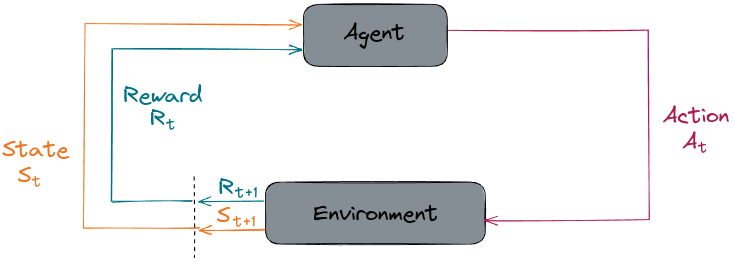
\includegraphics[width=0.7\linewidth]{mdp1}
\caption{Agent Environment interaction in the Reinforcement Learning Model.}
\label{fig:mdp1}
\end{figure}

% \par\noindent\rule{\textwidth}{0.4pt}
 The action space represents the possible actions that the agent can take in a given state. In the past, the tabular approach was used to store state and action values. However, in environments with a large number of states or actions, the approximation approach has replaced the tabular method. Neural networks are commonly used as approximation methods. There are two types of action spaces:
 \begin{itemize}
\item \textbf{ Discrete action space:} A discrete action space is one in which the set of possible actions is finite and well-defined. The agent can choose only one of the available actions at a time. For example, in a game of tic-tac-toe, the action space consists of the nine possible positions on the board where a player can place their mark ($X$ or $O$). This is a discrete action space because there are a finite number of possible actions (9) and the actions are well-defined (placing a mark in a specific location on the board).
\item \textbf{ Continuous action space:} A continuous action space is one in which the set of possible actions is infinite and not well-defined. The agent can choose any action within a continuous range of values. For example, in a self-driving car scenario, the action space might consist of the possible steering angles and accelerations that the car can take at any given moment. This is a continuous action space because the possible actions are not well-defined, as the car can take any steering angle or acceleration within a continuous range of values.
 \end{itemize}

% \par\noindent\rule{\textwidth}{0.4pt}
Deep Reinforcement Learning (DRL) is a field of study in which neural networks are utilized as function approximators to improve the performance of RL. Recently, several DRL techniques have achieved remarkable success in learning complex behavior skills and solving challenging control tasks in high-dimensional state-space \cite{28_wu2017scalable} environments. However, many benchmarked environments such as Atari \cite{29_mnih2013playing} and Mujoco \cite{30_todorov2012mujoco} lack complexity or realism, which is often present in robotics. Additionally, these benchmarked environments \cite{31_nogueira2017autonomously} do not use commonly used tools in the field such as ROS.
The research conducted in the previous work requires a considerable amount of effort for each specific robot, and therefore, the scalability of previous methods for modular robots is questionable. Consequently, trial and error learning process is often needed to apply the previous research to real-world robots. Training robotic arms to carry out certain actions, including touching an object in a virtual environment, is an intriguing use of RL. The robotic arm in this scenario must navigate a complicated state space while selecting actions that would maximize its reward while avoiding collisions with the environment. 

\subsubsection{Deep Reinforcement Learning}
Deep Reinforcement Learning (DRL) leverages deep learning architectures as function approximators to tackle high-dimensional data and address the challenge of approximating in the presence of large state and action spaces \cite{32_boute2022deep}. Unlike traditional methods such as decision trees or SVMs, DRL employs neural networks to map states to actions, enabling it to handle high-dimensional data types such as images, videos, and time-series data. The approach also utilizes deep learning techniques such as convolutional or recurrent neural networks to address the limitations of traditional artificial neural networks which are unable to handle such data and often ignore input data topology. Prior research has focused on addressing various challenges in applying DRL to different fields, particularly control problems and games like Atari. Some of the key tasks involved in DRL include:
\begin{itemize}
\item  \textbf{Exploration Exploitation: }The exploration refers to trying a new action, whereas exploitation makes use of learned knowledge to decide the action.
\item \textbf{Generalization:} Generalization, on the other hand, refers to the capability of the agent to adapt to new environments, which can range from one task to another or from simulation to a real-life situation.
\item \textbf{Finding Policy:} Finding a valuable policy involves identifying important states and actions that can help in learning an optimal policy for decision-making.
\item \textbf{Finding a catastrophe:} Discovering a catastrophic event is crucial, as such events may cause significant harm. These events may include physical harm, offensive tweets, false stories, and so on. Avoiding such occurrences can help to improve the policy.
\item \textbf{Handling Overestimation:} Overestimation occurs when inaccurate computation of action value takes place, often due to the use of the max operation in Q learning. It is important to handle overestimation to ensure that accurate values are computed.
\item \textbf{Reducing Sample Size:} Deep reinforcement learning (DRL) requires a large number of samples for effective training, which may not always be feasible in real-world scenarios. This poses a challenge for DRL applications that deal with limited data availability.
\item \textbf{Detection and prevention of overfitting:} overfitting is a common issue in DRL, especially when using high-capacity deep learning models. Overfitting occurs when the agent is too sensitive to small perturbations in the environment.
\item \textbf{Robust Learning:} In recent years, there has been a growing interest in incorporating robustness into the DRL system using techniques such as deep learning. Researchers have proposed various adversarial attacks and defense mechanisms to address this challenge. Therefore, enhancing the robustness of DRL systems has become an active research topic in the community.
\end{itemize}
 
The field of Reinforcement Learning (RL) has seen significant contributions from various researchers who have proposed different network architectures and action selection criteria. Some methods include trial and error without human intervention, learning via demonstrations, learning via criticism, and learning with adversaries to tackle complex problems. Despite these advancements, the challenge of discovering an optimal policy that is both robust and able to meet multiple goals remains a topic of active research and an open area of investigation.

%The simulated robotic arm used in this study consists of three joints, each of which can rotate through an angle of 360 degrees
%\cite{35_megalingam2013kinect}. The objective of the arm is to reach a target position specified by the RL algorithm. The state of the arm is represented by the joint angles, and the action is the change in joint angles to reach the target position. The reward function is defined as the negative Euclidean distance between the current position of the arm and the target position. The implementation of Double Q-Learning involves maintaining two Q-functions, Q1 and Q2, which are updated alternately. In each update, one of the Q-functions is used to select the best action, while the other Q-function is used to evaluate the selected action. This approach reduces the overestimation of action values, leading to more accurate estimation of the optimal policy.
%When compared, the performance of Double Q-Learning with that of Q-Learning and the Double Q-Learning outperformed Q-Learning in terms of convergence speed and final performance. The Double Q-Learning algorithm was able to learn an effective control policy for the robotic arm, enabling it to reach the target position with high accuracy and minimal error. To further evaluate the effectiveness of Double Q-Learning, we conducted experiments to test its robustness to changes in the target position and the reward function. We found that Double Q-Learning was able to adapt to changes in the target position and reward function, demonstrating its ability to learn a robust control policy for the robotic arm.

\subsection{Reinforcement Learning Algorithms and The Markov Decision Process (MDP)}
Reinforcement learning (RL) methods are particularly well-suited for robotics applications, such as robotic arm control. RL algorithms learn to control the arm by picking actions that maximize a reward signal, which may be a measure of how successfully the arm performs a task or how far it progresses toward a goal. Here are some popular RL algorithms used in robotics and for operating robotic arms:

\begin{itemize}
\item \textbf{Deep Deterministic Policy Gradient (DDPG):} The Deep Deterministic Policy Gradient (DDPG) is an actor-critic method that is meant to handle continuous action spaces, which is vital for directing the movement of a robotic arm \cite{44_villegas2018neural}. It estimates the action-value function using a deterministic policy function and a critic network and has been effectively applied to tasks such as reaching and grasping.
\item \textbf{Trust Region Policy Optimization (TRPO):} TRPO is a policy optimization algorithm that is well-suited for jobs requiring precise and accurate control, such as managing the position of a robotic arm \cite{45_1_lim2020federated}, \cite{45_kim2020motion}. It employs a trust region strategy to guarantee that policy adjustments are not too significant, which aids in maintaining stability.
\item \textbf{Asynchronous Advantage Actor-Critic (A3C): }A3C is a scalable and efficient RL technique designed to teach robotic arms to do complicated tasks such as item manipulation in crowded surroundings \cite{46_han2023survey}. It explores the state space and updates the policy using numerous simultaneous agents, which can dramatically accelerate the learning process.
\item \textbf{Deep Neural Networks for Q-Learning:} Q-Learning is a value-based RL algorithm that learns to assess the worth of actions in a given state. When Deep Q-Networks (DQN) are merged with deep neural networks, they form Deep Q-Networks (DQN), which are particularly helpful for applications involving high-dimensional sensory input, such as vision-based control of a robotic arm \cite{47_gupta2021deep}.
\item \textbf{Proximal Policy Optimization (PPO):} PPO is a policy optimization algorithm that updates the policy using a clipped surrogate objective function \cite{48_schulman2017proximal}. It has been used effectively in a variety of robotics activities, including regulating the movement of a robotic arm to conduct pick-and-place operations.

\end{itemize}

\subsubsection{The Markov Decision Process (MDP)}
MDP is a framework for modeling decision-making issues when the consequence of an action is unknown \cite{49_delage2010percentile}. It is commonly used in the field of reinforcement learning to simulate issues like robotic arm control, autonomous vehicle navigation, and gameplay. The decision-making agent in a MDP interacts with the environment in discrete time steps. At each time step, the agent performs an action depending on the current state of the environment and is rewarded with a new state. The agent's purpose is to discover a policy that maximizes the cumulative reward over time.
To convert a situation to an MDP framework, we must first identify the MDP components: state space, action space, transition probabilities, and reward function. Here's a quick rundown of each component:
\begin{enumerate}
\item \textbf{The state space} is the collection of all conceivable states in which the environment can exist. The state space of a robotic arm might comprise variables such as the arm's position and orientation, the placement of items in the environment, and the status of any sensors or actuators.
\item \textbf{The action space} is the collection of all conceivable actions that the agent can do in a given condition. The action space for a robotic arm might comprise orders to move the arm in different directions, alter its hold on an item, or activate sensors.
\item \textbf{Transition Probabilities} indicate the possibility of a state changing when a certain action is done. The transition probabilities of a robotic arm can be affected by the physical qualities of the arm and the objects in the surroundings, as well as any noise or uncertainty in the sensors or actuators.
\item \textbf{The reward function} assigns a monetary incentive to each state-action pair that represents the agent's aim. The reward function for a robotic arm can offer a positive reward for successfully gripping an object, a negative reward for colliding with an impediment, and zero otherwise.
\end{enumerate}
Reinforcement learning algorithms use MDPs to learn how to make decisions in a sequential decision-making problem.
These are only a few examples of RL algorithms that have been employed in robotics and robotic arm control. The algorithm used will be determined by the specific job and surroundings, as well as the features of the robot and sensors. RL algorithms offer the potential to make robotic arms more independent and adaptable, allowing them to adapt to changing surroundings and tasks in real-time.

\subsubsection{The exploration and exploitation trade-off in RL}
The exploration-exploitation trade-off in Reinforcement Learning (RL) refers to the issue encountered by an agent when deciding whether to continue exploring the environment to obtain additional knowledge or exploit the information it has already received to maximize its rewards.
Exploration is the process of attempting new behaviors and evaluating their effects in order to understand more about the environment. It entails attempting actions that have never been attempted before or attempting previously attempted actions with a new parameter configuration. Exploitation, on the other hand, refers to the practice of maximizing the cumulative benefit by utilizing knowledge learned from prior acts. It entails doing behaviors that have provided high benefits in the past or are expected to bring high returns in the future.
In RL, the trade-off between exploration and exploitation is crucial because if the agent concentrates just on exploration, it may not get enough incentives to develop an effective strategy. On the other side, if the agent is overly focused on exploitation, it may miss out on learning about other feasible, but lesser-known, positive acts that could contribute to higher long-term benefits.
To balance the exploration-exploitation trade-off, several ways can be applied, including:
\begin{enumerate}
\item\label{epsilon-greedy} \textbf{Epsilon-greedy:} The agent chooses the action with the largest expected payoff with a probability of one minus epsilon ($1 - \epsilon$) and a random action with a probability of epsilon ($\epsilon$). This enables the agent to explore the environment while still taking advantage of actions with high expected returns.
\item \textbf{Upper Confidence Bound (UCB):} The action with the highest upper confidence bound is chosen, which is determined by the mean reward and the variance of the reward distribution \cite{50_kaufmann2012bayesian}. This method encourages the agent to investigate less-explored behaviors while continuing to exploit acts with greater predicted rewards.
\item \textbf{Thompson Sampling:} In this method, the agent keeps a probability distribution over the reward of each action and chooses an action based on a sample from that distribution. This technique strikes a balance between exploration and exploitation by choosing activities with a high likelihood of high rewards while also investigating actions with a low probability of high rewards.
\end{enumerate}


%\subsubsection{Double Q-Learning}

%The simulated robotic arm used in this study consists of three joints, each of which can rotate through an angle of 360 degrees
%\cite{35_megalingam2013kinect}. The objective of the arm is to reach a target position specified by the RL algorithm. The state of the arm is represented by the joint angles, and the action is the change in joint angles to reach the target position. The reward function is defined as the negative Euclidean distance between the current position of the arm and the target position. The implementation of Double Q-Learning involves maintaining two Q-functions, Q1 and Q2, which are updated alternately. In each update, one of the Q-functions is used to select the best action, while the other Q-function is used to evaluate the selected action. This approach reduces the overestimation of action values, leading to more accurate estimation of the optimal policy.
%When compared, the performance of Double Q-Learning with that of Q-Learning and the Double Q-Learning outperformed Q-Learning in terms of convergence speed and final performance. The Double Q-Learning algorithm was able to learn an effective control policy for the robotic arm, enabling it to reach the target position with high accuracy and minimal error. To further evaluate the effectiveness of Double Q-Learning, we conducted experiments to test its robustness to changes in the target position and the reward function. We found that Double Q-Learning was able to adapt to changes in the target position and reward function, demonstrating its ability to learn a robust control policy for the robotic arm.



\subsection{Double Deep Q Learning (DDQN)}\label{foundations:ddqn}
%The Q-learning algorithm, a well-liked RL method, has a version called double Q-learning \cite{33_ogunniyi2014energy}. The fundamental tenet of Q-learning is to acquire knowledge of a function $Q(s,a)$, which denotes the anticipated reward for performing action in a given state s. The agent employs this feature to determine the optimal course of action in each state. However, Q-learning may be hampered by an overestimation of the Q-values, which could result in ineffective policies. This problem is addressed by double Q-learning, which estimates the greatest expected reward by switching between two different Q-functions.
Double Deep Q Learning (DDQN) is a Q-Learning algorithm extension that overcomes Q-value overestimation in standard Q-Learning. DDQN is a DRL method that combines a deep neural network with the Q-Learning technique to develop an optimum policy for an agent to make decisions in an environment.
The Double Deep Q-Learning (DDQN) method is an extension of the classic Q-Learning algorithm, which is widely used in Reinforcement Learning (RL) for robotics and robotic arm control. Deep RL method DDQN combines two deep neural networks to estimate the Q-values of state-action pairings in an environment.
Q-Learning is a well-known RL method that may be used to identify the best policy for an agent in a given environment. The agent in Q-Learning attempts to learn a function $Q(s, a)$ that calculates the anticipated reward for doing an action in state $s$. The best policy is then found by choosing the action that maximizes the Q-value for a particular state. Q-Learning, on the other hand, can only be employed in tiny settings with a limited number of states and actions. It is unsuitable for big and complicated situations.
Deep Q-Learning (DQL) is a Q-Learning variant that uses a deep neural network to estimate Q-values for state-action pairings in vast and complicated contexts. DQL has been demonstrated to be successful in a variety of difficult contexts, including video games and robotic control. However, it has been discovered that DQL can occasionally overstate Q-values, resulting in poor strategies.
To overcome this issue, Double Deep Q-Learning (DDQN) was created, which estimates Q-values using two deep neural networks. One network, known as the target network, is used to produce Q-value targets, while the other, known as the policy network, is used to generate Q-value estimates. To promote training stability, the Q-value objectives are updated less frequently than the Q-value estimations. This method decreases overestimation and enhances algorithm convergence.
To further improve learning, DDQN also uses a technique called "replay memory". This involves storing the agent's experiences in a buffer and randomly sampling from the buffer to train the neural network. By doing so, the agent can learn from a more diverse set of experiences, rather than just learning from the most recent experience. 
The DDQN algorithm is summarized below:
\begin{enumerate}
\item  \label{itm:dqn_1} Initialize the replay memory buffer $D$ with capacity $N$.
\item Initialize the policy Q-network with random weights $\theta$.
\item Clone the policy Q-network and let that be the target Q-network with weights $\theta^{-} = \theta$.
\item For each episode $e=1,2,...,E$ do the following:
	\begin{enumerate}
	\item Initialize the environment with initial state $s_0$.
	\item For each step $t=1,2,...,T$ do the following:
		\begin{enumerate}
		\item With probability $\epsilon$ select a random action $a_t$, otherwise select $a_t=\arg\max_{a} Q(s_t, a; \theta)$.
		\item Execute action $a_t$ and observe reward $r_t$ and next state $s_{t+1}$.
		\item Store the experience $(s_t, a_t, r_t, s_{t+1})$ in the replay memory buffer $D$.
		\item Sample a mini-batch of experiences $(s_j, a_j, r_j, s_{j+1})$ from the replay memory buffer $D$.
		
		\item Compute the Q-learning target value for each experience $(s_j, a_j, r_j, s_{j+1})$:
		
		 $y_j = 
		 \begin{cases} 
		 r_j & \text{if episode terminates at step } j+1 \\ 
		 r_j + \gamma\max_{a'}Q(s_{j+1},a';\theta^{-}) & \text{otherwise} \end{cases}$.
		
		\item Compute the loss between the predicted Q-value and the target Q-value: $L(\theta) = \frac{1}{B}\sum_{j=1}^B(y_j-Q(s_j,a_j;\theta))^2$.
		\item Update the policy Q-network weights using gradient descent: $\theta \leftarrow \theta - \alpha\nabla_\theta L(\theta)$.
		\item Every $C$ steps update the target Q-network weights: $\theta^{-} \leftarrow \theta$.
		\item Update the current state, set $s_t=s_{t+1}$.
		\end{enumerate}
	\end{enumerate}
\end{enumerate}

%\begin{enumerate}
%\item Set up two deep neural networks, one for the target network and one for the policy network.
%\item Create a replay buffer to record the agent's experience tuples (state, action, reward, next state).
%\item Set the exploration strategy's parameters, such as the epsilon-greedy policy.
%\item For every episode:
%\begin{enumerate}
%\item Return the environment to its original state.
%\item Using the exploratory technique, choose an action.
%\item Carry out the activity and watch for the reward and the following state.
%\item Put the experience tuple into the replay buffer.
%\item Take a random sample of experience tuples from the replay buffer.
%\item Using the target network, compute the Q-value targets.
%\item Using the policy network, compute the Q-value estimations.
%\item Determine the difference between the Q-value objectives and the Q-value estimations.
%\item To minimize loss, update the online network via backpropagation.
%\item Periodically update the target network with the weights of the policy network.
%\item Repeat steps b–j until the episode is finished.
%\end{enumerate}
%\item Repeat step 4 for a fixed number of episodes or until the agent reaches a satisfactory level of performance.
%\end{enumerate}

There are various advantages of using DDQN over standard Q-Learning and DQL. It decreases overestimation, enhances stability, and speeds up convergence. DDQN is also capable of dealing with vast and complicated settings with multidimensional state and action spaces. These characteristics make DDQN an appealing candidate for robotic control applications.
DDQN may be used in robotics and robotic arm control to determine an optimum policy for the agent to complete certain tasks such as item grabbing or assembly. Without any prior understanding of the environment or the work, DDQN may be used to learn the policy from the ground up. The agent may investigate its surroundings and learn from its experiences in order to better its performance.

In this work, the simulated robotic arm would operate as the agent in a Double Q-learning framework, interacting with its surroundings and receiving rewards or punishments as a result of its actions. The orientation and position of the robotic arm, along with the location and characteristics of the object it is attempting to touch, would all be included in the state space. The robotic arm's range of potential motions for approaching the object would make up the action space. The goal of the reward function is to persuade the robotic arm to touch the target without causing a collision or any other unfavorable outcomes.
The Double Q-learning method is used by the robotic arm to investigate its environment during training and modify its Q-functions in response to incentives. By estimating the expected reward for every action using the two Q-functions, the algorithm would select the action featuring the largest expected reward. The robotic arm would develop a policy that enables it to consistently touch the target by continuing this process over a large number of attempts. In next chapters, we explore and present results for the use of Double Q-Learning in a simulated robotic arm to learn effective control policies for the arm.
%\hrule 

%In subsequent chapters, you can reference this one to avoid having to explain everything over and over again. This means that you just include things here that are necessary for the understanding of later chapters, nothing more.
%\subsection{Topic 01}\label{sec:grundlagen1}
%\hrule
%
\section{Implementation}\label{sec:umsetzung}
\subsection{Environment Preparation}\label{sec:env-preparation}
A SDF file \ref{sdf} containing the object the robotic arm has to learn to touch was created and when launched in Gazebo, it looks like Figure \ref{fig:can}.

The robotic arm used in the simulation is the Kuka KR210. The necessary files to simulate such a robotic arm were taken from ~\cite{RoboND-Kinematics-Project}. From this repository, we need the \textit{DAE}, \textit{STL}, and \textit{URDF} files to make the robotic arm work.

To use the robotic arm in our simulation, the first step is to create a ROS 2 workspace and package to later place the simulation files in it; the simulation files and folders were placed in the directory structure in Figure \ref{fig:project_structure_1}.

Once we have the simulation files in place, we can test if we can see and interact with the robotic arm; for this, we use the \textit{ROS robot\_state\_publisher} node \ref{ros2-robot-state-publisher} and Rviz \ref{rviz_rqt}. The \textit{ROS robot\_state\_publisher} recieves the \textit{URDF} file content as a parameter and publishes it to a topic called \textit{/robot\_description}. Then to visualize the robot we use RViZ which would subscribe to \textit{/robot\_description} topic and render the robotic arm. The result can be seen in Figure \ref{fig:kuka1}.

The communication between the \textit{robot\_state\_publisher} node, the \textit{/robot\_description} topic and \textit{RViz} can be seen in Figure \ref{fig:rosgraph1}. 
\begin{figure}[H]
  \centering
 % 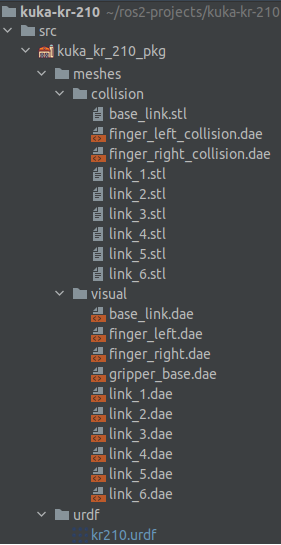
\includegraphics[width=0.3\linewidth]{project_structure_1}
  \subfloat[Can described in the SDF file in Gazebo which is the object to be touched by the robotic arm.]{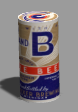
\includegraphics[width=0.47\textwidth]{can}\label{fig:can}}
  \hfill
  \subfloat[Project structure after copying the \textit{DAE}, \textit{STL}, and \textit{URDF} files into our package.]{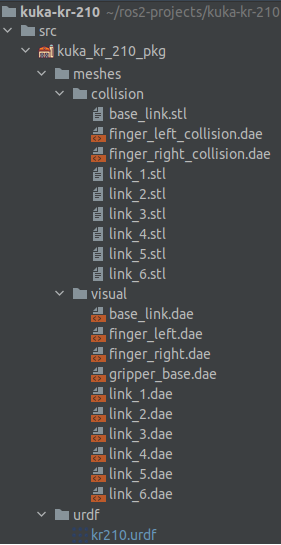
\includegraphics[width=0.35\textwidth]{project_structure_1}\label{fig:project_structure_1}}
  \caption{World created in Gazebo and starting directory structure after copying the robotic arm simulation files.}
\end{figure}

\begin{figure}[H]
	\centering
	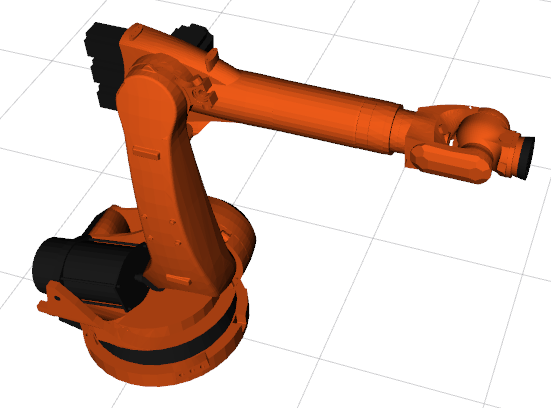
\includegraphics[width=0.7\linewidth]{kuka1}
	\caption[Rviz2 kuka]{Kuka KR210 in RViz2.}
	\label{fig:kuka1}
\end{figure}

\begin{figure}[H]
\centering
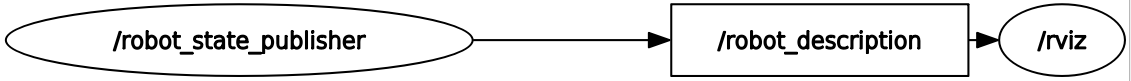
\includegraphics[width=0.9\linewidth]{rosgraph1}
\caption[The robot\_state\_publisher node]{The ROS \textbf{robot\_state\_publisher} node takes the URDF file content and publishes it to the \textbf{/robot\_description} topic to which Rviz subscribes and gets the robotic arm information to finally show it.}
\label{fig:rosgraph1}
\end{figure}

The robotic arm Kuka KR210 consists of seven and links six joints that connect them. 

The six joints of the KR210 are numbered J1 to J6 as can be seen in Figure \ref{fig:kuka5}, and they allow the robot to move in various directions and orientations.
\begin{itemize}
	\item \textbf{J1:}\label{joint:j1} The first joint is the base joint, which allows the robot to rotate horizontally around its vertical axis.
	
	\item \textbf{J2:}\label{joint:j2} The second joint is the shoulder joint, which allows the robot to lift and lower its arm vertically.
	
	\item \textbf{J3:}\label{joint:j3} The third joint is the elbow joint, which allows the robot to bend its arm vertically.
	
	\item \textbf{J4:}\label{joint:j4} The fourth joint is the wrist roll joint, which allows the robot to rotate its wrist around its vertical axis.
	
	\item \textbf{J5:}\label{joint:j5} The fifth joint is the wrist pitch joint, which allows the robot to tilt its wrist up and down.
	
	\item \textbf{J6:}\label{joint:j6} The sixth joint is the wrist yaw joint, which allows the robot to rotate its wrist horizontally.	 
\end{itemize}

\begin{figure}[H]
	\centering
	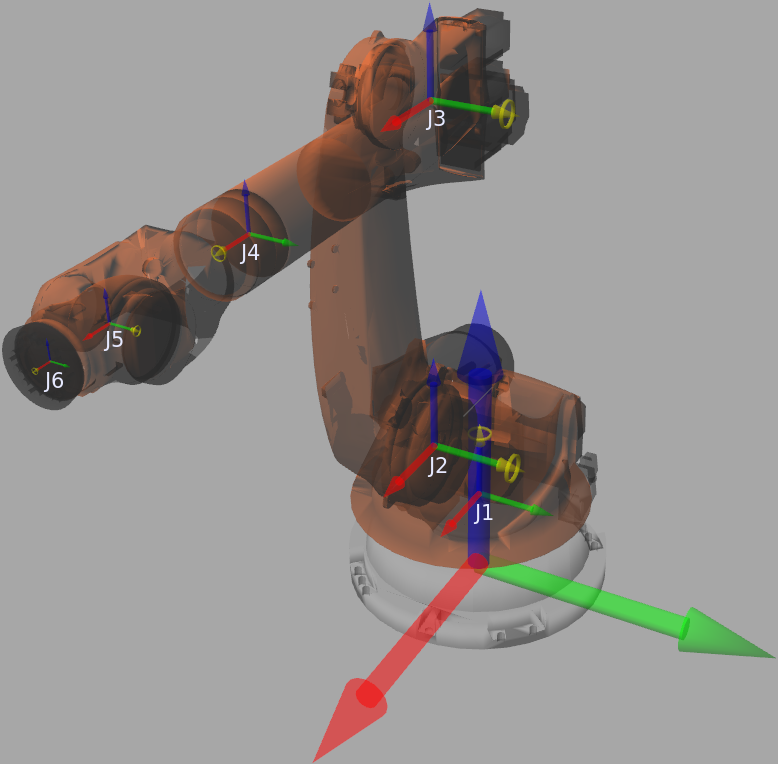
\includegraphics[width=0.9\linewidth]{kuka5}
	\caption[Joints in the Kuka KR210.]{Joints and axis around which they allow movement in the Kuka KR210 arm.}
	\label{fig:kuka5}
\end{figure}

The arm also has links which are connected by the joints; the links of the kuka KR210 are: the base, the lower arm, the upper arm, the wrist, and the end effector. These links are designed to provide strength and rigidity to the robot arm while allowing for smooth and precise movement. These links can be seen in Figure \ref{fig:kuka7} and are:

\begin{itemize}
	\item \textbf{Base Link:} The base link connects the robotic arm to the fixed base or mounting structure. It provides stability and support. In our simulation it is attached to the ground.
	
	\item \textbf{Link 1:} Also known as the shoulder link, it connects the base link to the upper arm. It is responsible for the vertical movement of the upper arm and enables the arm to raise and lower. This is the first link that connects the base link via joint 1 (J1 in \ref{joint:j1}) in one end and joint 2 (J2 in \ref{joint:j2}) in the other end.
	
	\item \textbf{Link 2:} Also known as the upper arm link, it extends from the shoulder link to the elbow joint (J3 in \ref{joint:j3}). It is a rigid segment that allows for vertical and horizontal movements, providing reach and positioning capability. This link is between the joint 2 (J2 in \ref{joint:j2}) and the joint 3 (J3 in \ref{joint:j3}).
	
	\item \textbf{Link 3:} Also known as the forearm link, it extends from the elbow joint (J3 in \ref{joint:j3}) to the wrist roll joint (J4 in \ref{joint:j4}). It is a rigid segment that helps transmit motion and provides structural support.
	
	\item \textbf{Link 4: }This link extends from joint 3 (J3 in \ref{joint:j3}) to joint 4 (J4 in \ref{joint:j4}).
	
	\item \textbf{Link 5: }This link extends from joint 4 (J4 in \ref{joint:j4}) to joint 5 (J5 in \ref{joint:j5}).
	
	\item \textbf{End Effector (Link 6):} This is the tool or gripper attached to the last joint. It is the component that directly interacts with objects or the environment, enabling the arm to perform specific tasks.
	
\end{itemize}

\begin{figure}[H]
  \centering
  \subfloat[Links 1, 3 and 5 in the Kuka KR210.]{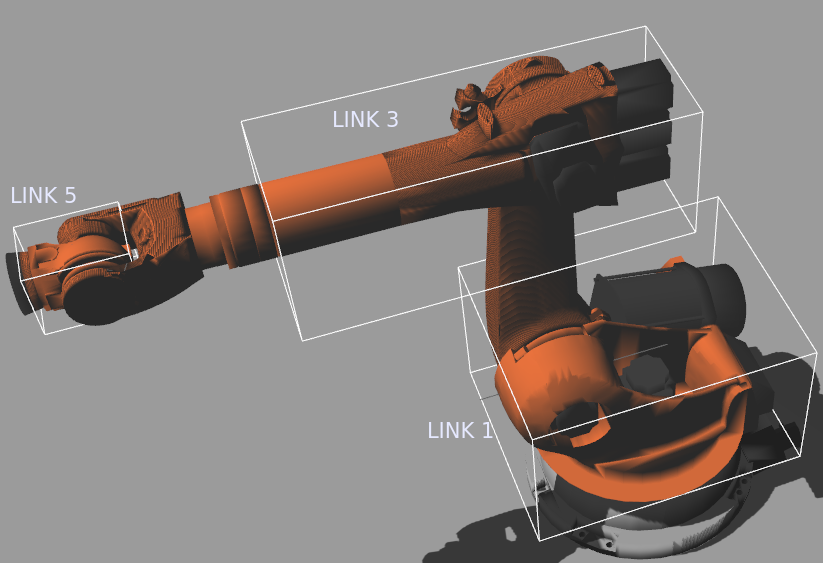
\includegraphics[width=0.45\textwidth]{kuka6}\label{fig:kuka6}}
  \hfill
  \subfloat[Base Link, Link 2, 4 and 6 in the Kuka KR210.]{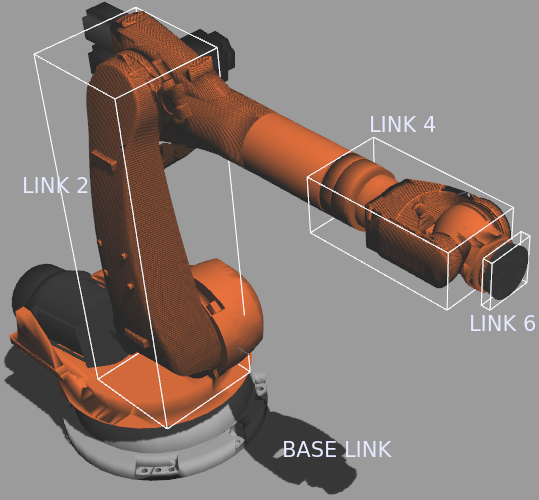
\includegraphics[width=0.45\textwidth]{kuka7}\label{fig:kuka7}}
  \caption{Links in the Kuka KR210.}
\end{figure}

After setting up the robotic arm, the next step is to add sensors to it, and to configure them to work with ROS 2 and Gazebo.
\begin{itemize}
\item To detect collisions between the robotic arm and the object it should learn to touch, a bumper sensor is added to links 4, 5, and 6. This is done by adding the code in Listing \ref{bumperSensorXml} to the \textit{URDF} file.

\item A camera is added to the \textit{URDF} file as well, this is done by adding the code in Listing \ref{cameraSensorXml} to the \textit{URDF} file.

\item In the \textit{SDF} file, the Gazebo ROS state plugin was added. This is done by adding the code in Listing \ref{gazeboRosStatePluginXml} in the \textit{SDF} file. This plugin not only allows us to monitor our models' positions and velocities but also modify them programmatically.
\end{itemize}

Once the robotic arm and the sensors are in place, the next step is to launch our \textit{SDF} file in Gazebo and spawn the robotic arm into the world to finally have our setup as in Figure \ref{fig:kuka4}

\begin{figure}[H]
	\centering
	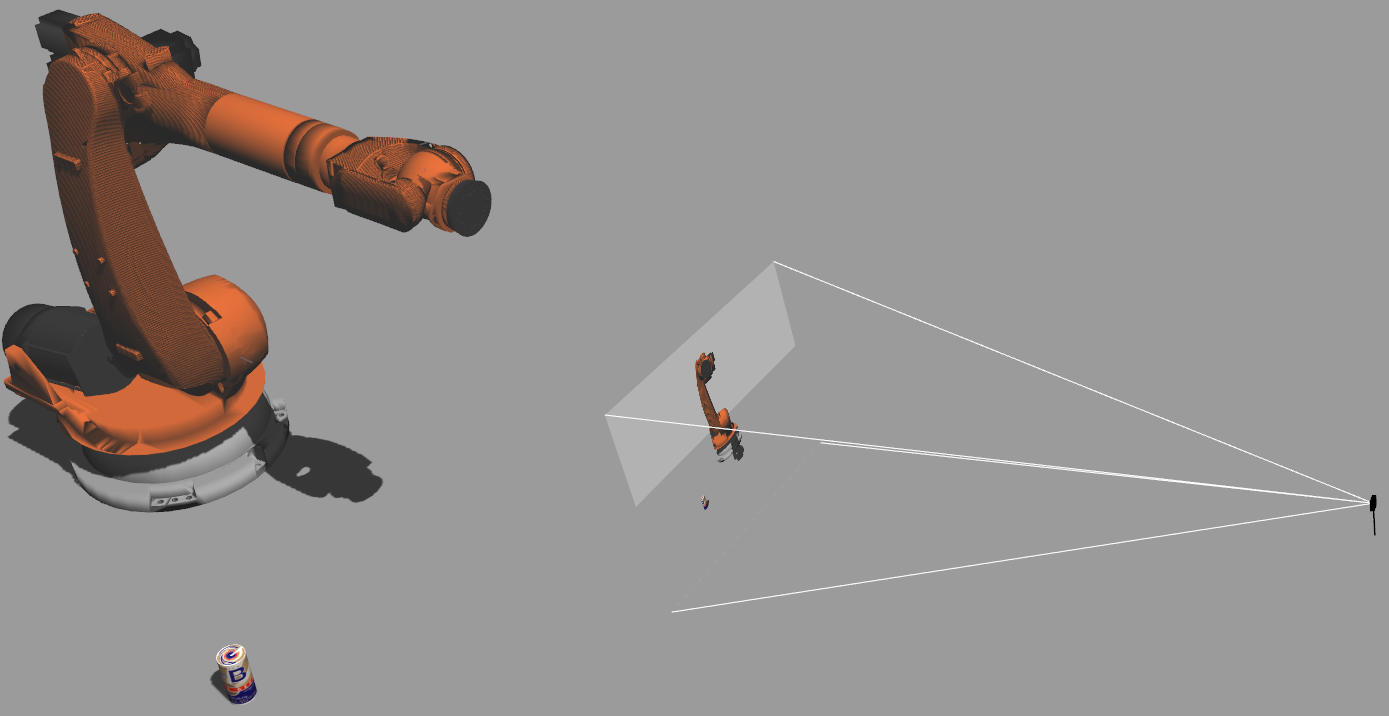
\includegraphics[width=0.95\linewidth]{kuka4}
	\caption[Gazebo World.]{Gazebo world containing the robotic arm, the object to be touched, plus the sensors and plugins added.}
	\label{fig:kuka4}
\end{figure}

A launch file was created to spawn the robotic arm in the gazebo world with the can as in Figure \ref{fig:kuka4}. Furthermore, the ROS nodes and topics in figures \ref{fig:rosgraph00}, \ref{fig:rosgraph01}, \ref{fig:rosgraph02}, \ref{fig:rosgraph03}, \ref{fig:rosgraph04} are initialized to be used later.


\begin{figure}[H]
\centering
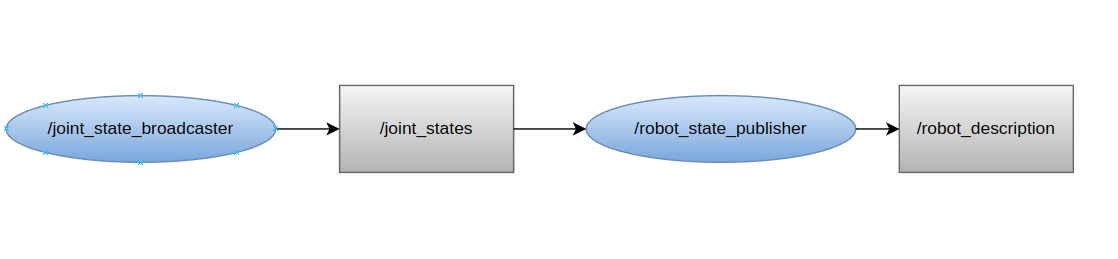
\includegraphics[width=0.95\linewidth]{rosgraph00}
\caption[The joint\_state\_broadcaster node.]{The joint state broadcaster node publishes the current state of each joint in the robot's body to the ROS (Robot Operating System) network. This state includes the joint's position, velocity, and effort (torque) values. }
\label{fig:rosgraph00}
\end{figure}
 
\begin{figure}[H]
\centering
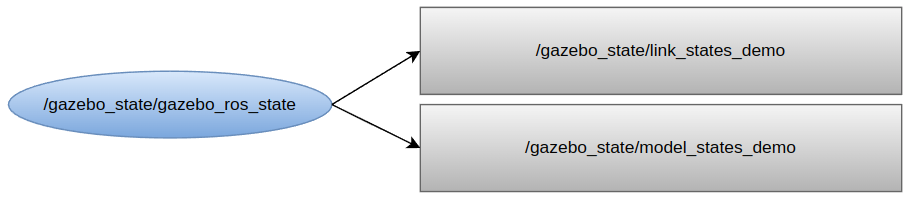
\includegraphics[width=0.95\linewidth]{rosgraph01_n}
\caption[The gazebo\_ros\_state node.]{The node \textit{/gazebo\_state/gazebo\_ros\_state} publishes the state of the models in the gazebo world to the topics \textit{/gazebo\_state/link\_states\_demo} and \textit{/gazebo\_state/model\_states\_demo} as specified in Listing \ref{gazeboRosStatePluginXml}}
\label{fig:rosgraph01}
\end{figure}

\begin{figure}[H]
\centering
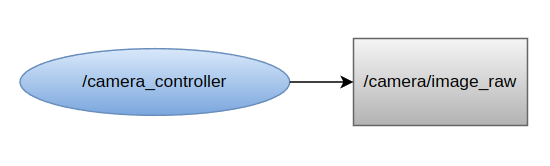
\includegraphics[width=0.95\linewidth]{rosgraph02_new}
\caption[The camera\_controller node.]{As a result of adding Listing \ref{cameraSensorXml} a node \textit{camera\_controller} is created and it publishes to the topics \textit{/camera/image\_raw}.}
\label{fig:rosgraph02}
\end{figure}

\begin{figure}[H]
\centering
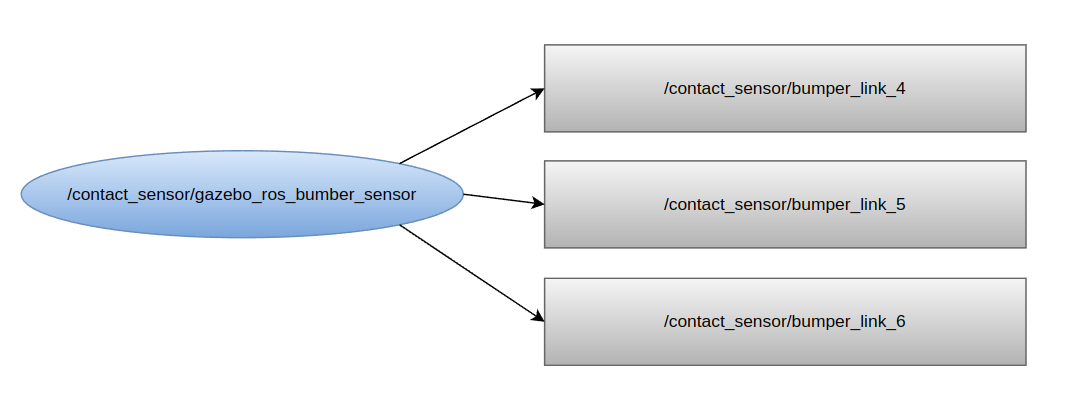
\includegraphics[width=0.95\linewidth]{rosgraph03_new}
\caption[The /contact\_sensor/gazebo\_ros\_bumper\_sensor node.]{As a result of adding Listing \ref{bumperSensorXml} there are \textit{/contact\_sensor/gazebo\_ros\_bumper\_sensor} nodes publishing the collision details to the topics \textit{/contact\_sensor/bumper\_link\_4}, \textit{/contact\_sensor/bumper\_link\_5}, and\textit{ /contact\_sensor/bumper\_link\_6}. }
\label{fig:rosgraph03}
\end{figure}

\begin{figure}[H]
\centering
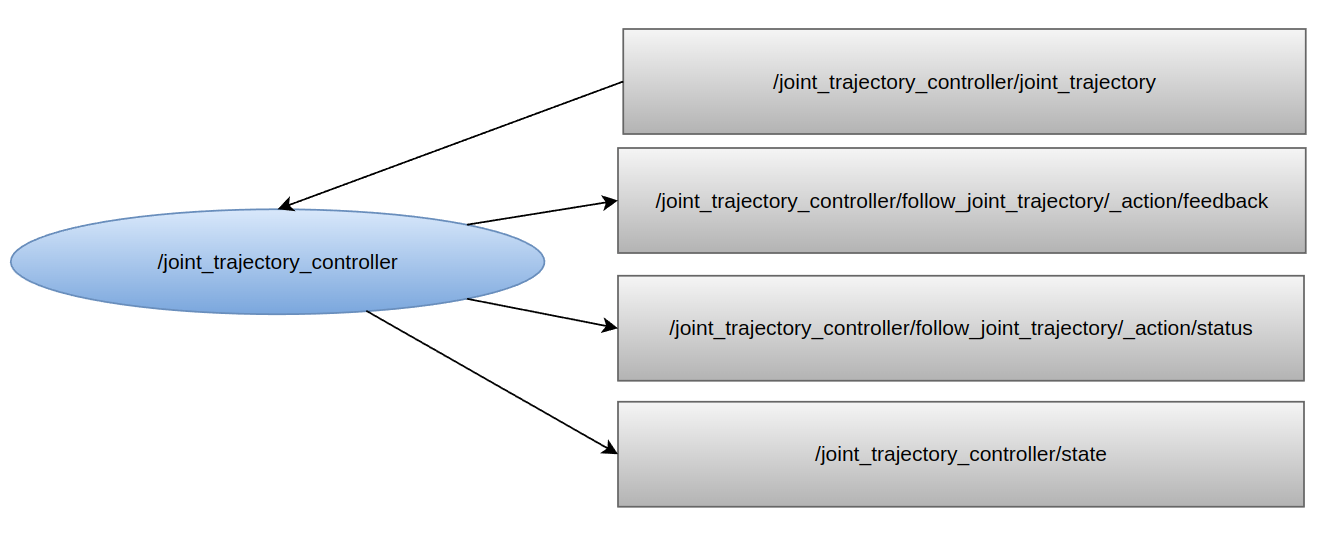
\includegraphics[width=0.95\linewidth]{rosgraph04_new}
\caption[The /joint\_trajectory\_controller node.]{The joint trajectory controller node is responsible for generating and executing a trajectory plan for the robot's joints. This is the node used to send the desired positions when controlling the robotic arm.}
\label{fig:rosgraph04}
\end{figure}

With the robotic arm spawn and the nodes and topics running to interact with it, the next step is to create the classes that define the reinforcement learning environment.

Figure \ref{fig:classdiagramcomplete} is a description of the classes and relationships used to conduct the experiments.

\begin{figure}[H]
\centering
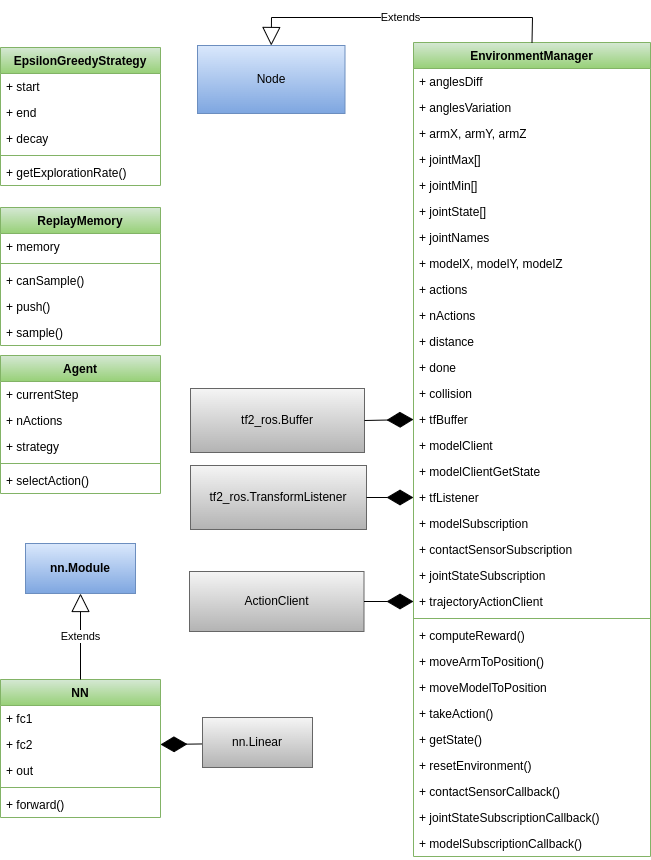
\includegraphics[width=0.95\linewidth]{uml_diagram_complete}
\caption[Classes and relationships in the reinforcement learning framework.]{Classes defining the reinforcement learning framework that will run the environment experiments for the arm to learn to touch the object.}
\label{fig:classdiagramcomplete}
\end{figure}

\subsection{The NN class}      
The NN class in Figure \ref{fig:classdiagramcomplete} implements the neural network used in this framework, i.e. our DQN.         
PyTorch \cite{pytorch} is used for the neural network, specifically the \textit{nn.Module}. 
The $nn$ package contains a Module class which serves as the foundation for all neural network modules. This means that the used network and its layers will inherit from the Module class. To implement the neural network, the NN class that extends the nn.Module class is created. The neural network will be fed the current state ($s$) as follows:
\begin{align}
		s &= input = (\theta_1, \theta_2, \theta_3, d) \label{eq:1}
\end{align}

where, $\theta_1, \theta_2, and \theta_3$ represent the joint angles of the robotic arm (J1, J2, and J3 in Figure \ref{fig:kuka5}), and $d$ represents the distance between the end effector of the arm and the object. 


%The main components are:
%\begin{itemize}
%\item The action space is defined as angle variations of 0.03 radians for the Joints 1, 2 and 3. That is a space of 3 dimensional vectors whose components can only be three possible values (i.e. -0.03, 0, and 0.03).
%\item The state space consists of four dimensional vectors whose components are the angle values of Joints 1, 2, and 3, and the distance between Link 6 and the object the arm has to touch.
%\item The function computeReward in the EnvironmentManager class takes care of computing the reward, it is executed when the function takeAction in the EnvironmentManager class is executed. The computeReward function is as follows: 
%
%$reward = 
% \begin{cases} 
% 	100 	& \text{if the arm touches the object.} \\ 
% 	1 		& \text{if episode terminates at step.} \\ 
% 	-1 		& \text{if the arm moves away from the object.} 
% \end{cases}$
%
%\item The ReplayMemory class keeps record of experiences, for every step it records the current state, the action taken, the reward, and the new state.
%\item The EpsilonGreedyStrategy class provides the exploration probability, at the beginning the exploration probability is high and as the simulation continues this is defined to decay up to a minimum, at which point mostly exploitation is done.
%\item The class NN defines the neural network used. The one used has two hidden layers with 32 and 64 nodes and ReLU as the activation function. The input and output layers are defined by the dimension of the state space and the number of actions in the action space respectively.
%\item The Agent class takes care of selecting an action based on the exploration probability given by the EpsilonGreedyStrategy class.
%
%\end{itemize} 

%\subsection{The Double Deep Q Learning Algorithm}
%Once we have our environment prepared, we are ready to implement the following Deep Q Learning Algorithm:
%\begin{enumerate}
%\item  \label{itm:dqn_1} Initialize the replay memory buffer $D$ with capacity $N$.
%\item Initialize the policy Q-network with random weights $\theta$.
%\item Clone the policy Q-network and let that be the target Q-network with weights $\theta^{-} = \theta$.
%\item For each episode $e=1,2,...,E$ do the following:
%	\begin{enumerate}
%	\item Initialize the environment with initial state $s_0$.
%	\item For each step $t=1,2,...,T$ do the following:
%		\begin{enumerate}
%		\item With probability $\epsilon$ select a random action $a_t$, otherwise select $a_t=\arg\max_{a} Q(s_t, a; \theta)$.
%		\item Execute action $a_t$ and observe reward $r_t$ and next state $s_{t+1}$.
%		\item Store the experience $(s_t, a_t, r_t, s_{t+1})$ in the replay memory buffer $D$.
%		\item Sample a mini-batch of experiences $(s_j, a_j, r_j, s_{j+1})$ from the replay memory buffer $D$.
%		
%		\item Compute the Q-learning target value for each experience $(s_j, a_j, r_j, s_{j+1})$:
%		
%		 $y_j = 
%		 \begin{cases} 
%		 r_j & \text{if episode terminates at step } j+1 \\ 
%		 r_j + \gamma\max_{a'}Q(s_{j+1},a';\theta^{-}) & \text{otherwise} \end{cases}$.
%		
%		\item Compute the loss between the predicted Q-value and the target Q-value: $L(\theta) = \frac{1}{B}\sum_{j=1}^B(y_j-Q(s_j,a_j;\theta))^2$.
%		\item Update the policy Q-network weights using gradient descent: $\theta \leftarrow \theta - \alpha\nabla_\theta L(\theta)$.
%		\item Every $C$ steps update the target Q-network weights: $\theta^{-} \leftarrow \theta$.
%		\item Update the current state, set $s_t=s_{t+1}$.
%		\end{enumerate}
%	\end{enumerate}
%\end{enumerate}

A simple neural network with two fully connected layers and an output layer is used.
\begin{listing}[htbp]
\caption{Implementation of the Deep Neural Network.}
\label{code:nn_class_1}
\begin{tcolorbox}[]
\begin{minted}[fontsize=\scriptsize]{python}
 class NN(nn.Module):
     def __init__(self, nInputs=4, nOutputs=27):
         super().__init__()
         # input current angles and distance
         self.fc1 = nn.Linear(nInputs, out_features=32)
         self.fc2 = nn.Linear(in_features=32, out_features=64)
         self.out = nn.Linear(in_features=64, out_features=nOutputs)
\end{minted}
\end{tcolorbox}
\end{listing} 

In listing \ref{code:nn_class_1}, the fully connected layers are referred to as $Linear$ layers in PyTorch.

The first Linear layer will accept input with dimension of four. This first layer will generate 32 outputs, which will serve as the input for the second Linear layer. The second Linear layer will have 64 outputs, and the output layer will have 27 outputs, taking 64 inputs from the previous layer.

The network outputs \textit{Q-values} that correspond to each possible action that the agent can take from a given state. Note that the network used does not have convolutional layers because no image processing takes place.
The final step in defining the NN class is to create a function called $forward()$. This function will carry out a forward pass through the network. It's important to keep in mind that $forward()$ is a necessary function for all PyTorch neural networks.

\begin{listing}[htbp]
\caption{Implementation of the $forward()$ function needed for the DQN.}
\label{code:nn_class_2}
\begin{tcolorbox}[]
\begin{minted}[fontsize=\scriptsize]{python}
def forward(self, s):
    s = F.relu(self.fc1(s))
    s = F.relu(self.fc2(s))
    s = self.out(s)
    return s
\end{minted}
\end{tcolorbox}
\end{listing} 
When the network receives a state $s$; it passes it to the first fully connected layer and applies $relu$ to the output before sending it to the second fully connected layer. After that, $relu$ is applied before passing the result to the output layer. The $forward()$ function then returns the result obtained from the output layer.

\subsection{The Replay Memory class}
To define the $ReplayMemory$ class, the Experience class which defines $Experience=(s_j, a_j, r_j, s_{j+1})$ is used. An experience contains the current state($s_j$), the action taken in that state ($a_j$), the reward for the action taken ($r_j$), and the next state of the environment ($s_{j+1}$). To create an instance of the $ReplayMemory$ class, $capacity$ is the only parameter needed.
\begin{listing}[htbp]
\caption{Implementation of the Replay Memory class.}
\label{code:replay_memory}
\begin{tcolorbox}[]
\begin{minted}[fontsize=\scriptsize]{python}
class ReplayMemory:
    def __init__(self, capacity):
        self.memory = deque(maxlen=capacity)
    def push(self, experience):
        self.memory.append(experience)
    def sample(self, batchSize):
        return random.sample(self.memory, batchSize)
    def canSample(self, batchSize):
        return len(self.memory) >= batchSize
\end{minted}
\end{tcolorbox}
\end{listing} 

The code in Listing \ref{code:replay_memory} implements the $ReplayMemory$ class. When $ReplayMemory$ is instantiated, its capacity is initialized to $capacity$, and the $memory$ attribute is defined as a \textbf{deque} data type \ref{python:deque}. To add and store $experiences$ the $push$ function is defined, which is just a wrapper for the append built-in function. When the number of experiences in $memory$ reaches $capacity$, new experiences are kept and old ones are removed. The $sample()$ function provides a batch of random experiences which is used to train the neural network. Finally, the function $canSample()$ tells us whether we can sample from memory or not.

\subsection{The Epsilon Greedy Strategy class}
To balance exploration and exploitation the epsilon greedy strategy is used. An exploration rate called $epsilon$ is defined. Epsilon is the probability that the agent will choose a random action (exploration). An $epsilon$ value of one means that the agent will only explore the environment. As the agent learns, $epsilon$ decays by a defined decay rate;  meaning that the agent will no longer just explore, but also use what is has learned about the environment or exploit.
\begin{listing}[H]
\caption{Implementation of the $EpsilonGreedyStrategy$ class.}
\label{code:epsilon-greedy}
\begin{tcolorbox}[]
\begin{minted}[fontsize=\scriptsize]{python}
class EpsilonGreedyStrategy:
    def __init__(self, start, end, decay):
        self.start = start
        self.end = end
        self.decay = decay
    def getExplorationRate(self, currentStep):
        return self.end + (self.start - self.end) * math.exp(-1. * currentStep * self.decay)
\end{minted}
\end{tcolorbox}
\end{listing} 
In Listing \ref{code:epsilon-greedy}, $start$, $end$, and $decay$ correspond to the starting, ending, and decay rate for $epsilon$. The function $get_exploration_rate()$ has the $currentStep$ of the agent as parameter and returns the calculated exploration rate.

\subsection{The Agent class}
The implemented $Agent$ class in Listing \ref{code:agent} has $strategy$ and $nActions$ parameters as inputs in its constructor. An instance of the $EpsilonGreedyStrategy$ class is used for the $strategy$ variable in order to create the agent object. The $nActions$ parameter refers to the number of possible actions that the agent can take in a given state. In our case, this number is twenty seven; all possible actions for the agent in a given state are written in Equation \ref{eq:action-space}.

\begin{listing}[H]
\caption{Implementation of the Agent class.}
\label{code:agent}
\begin{tcolorbox}[]
\begin{minted}[fontsize=\scriptsize]{python}
class Agent:
    def __init__(self, strategy, nActions):
        self.strategy = strategy
        self.nActions = nActions
        self.currentStep = 0
    def selectAction(self, state, policyNetwork):
        rate = self.strategy.getExplorationRate(self.currentStep)
        self.currentStep += 1
        if rate > random.random():  # explore
            action = torch.tensor([random.randrange(self.nActions)])
        else:  # exploit
        	with torch.no_grad():
            	action = policyNetwork(state).argmax(dim=1)
        return action
\end{minted}
\end{tcolorbox}
\end{listing} 

The parameter $currentStep$ is set to zero at the beginning and indicates the current iteration of the agent in the environment.

The policy network refers to a deep Q-network that is trained to learn the optimal policy.

Inside the $selectAction()$ function, the $rate$ variable is set to the exploration rate returned from the $EpsilonGreedyStrategy$ object that was passed in when creating the agent object; and the $currentStep$ attribute of the agent is incremented by 1. 
Then, we check whether the $rate$ variable is greater than a random number generated between 0 and 1. If it is, we explore the environment by randomly selecting an action from our action space $A$. If not, we exploit the environment by selecting the action that corresponds to the highest Q-value output from our policy network for the given state. To perform inference, the $torch.no\_grad()$ method is used to turn off gradient tracking since the model is only used for prediction, not training. During training, PyTorch tracks all the forward pass calculations that occur within the network. By turning off gradient tracking,  PyTorch does not to keep track of any forward pass calculations.

\subsection{The Environment Manager class}

Finally the class that manages the environment is the $EnvironmentManager$ class. This class implements the $rclpy.node.Node$ class in Python in order to create a node in our ROS 2 framework and interact with the other nodes in the environment.
The following properties are initialized when the $EnvironmentManager$ class is instantiated:
\begin{enumerate}
\item The $done$ property indicates whether the episode has finished or not. An episode ends when there is a collision between the end effector, the Link 5, or the Link 6 of the arm and the target object or when the episode has reached its maximum defined number of steps.
\item\label{env-manager:distance} The $distance$ property stores the latest distance between the end effector of the arm and the object.
\item\label{env-manager:arm-coordinates} The $armX$, $armY$, and $armZ$ properties store the latest $(x, y, z)$ coordinates of the end effector of the arm.
\item The $joint1State$, $joint2State$, $joint3State$, $joint4State$, $joint5State$, and $joint6State$ properties store the latest angles of the arm joints of the same name. 
\item The $joint1Max$, $joint1Min$, $joint2Max$, $joint2Min$, $joint3Max$, and $joint3Min$ properties define the maximum each joint can move without causing collisions within the arm or with the floor. These values were found using Rviz \ref{rviz_rqt}.
\item The $tfBuffer = tf2\_ros.Buffer()$ and

$tfListener = tf2\_ros.TransformListener(self.tfBuffer, self)$ properties are defined in order to calculate the $armX$, $armY$, and $armZ$ properties in ~\ref{env-manager:arm-coordinates}.
\item\label{env-manager:angle-diff} The $angleDiff$ property defines how much each joint's angle can vary per step per episode in radians.
\item The $anglesVariation$ property defines the possible movements for each joints. Each joint can move $-angleDiff$, $0$, or $+angleDiff$ rads.
\item The $actions$ property stores all the possible actions in the action space $A$
\item The $nActions$ property stores the number of actions in the action space $A$. The action space is defined as:
\begin{equation}
  \begin{aligned}
A = \{(-\theta, -\theta, -\theta), (-\theta, -\theta, 0), (-\theta, -\theta, \theta), (-\theta, 0, -\theta), (-\theta, 0, 0), (-\theta, 0, \theta),\\
 (-\theta, \theta, -\theta), (-\theta, \theta, 0), (-\theta, \theta, \theta), (0, -\theta, -\theta), (0, -\theta, 0), (0, -\theta, \theta),(\theta, \theta, -\theta),\\
 (\theta, -\theta, -\theta), (\theta, -\theta, 0), (\theta, -\theta, \theta), (\theta, 0, -\theta), (\theta, 0, 0), (\theta, 0, \theta),(\theta, \theta, 0),\\
 (0, 0, -\theta), (0, 0, 0), (0, 0, \theta), (0, \theta, -\theta), (0, \theta, 0), (0, \theta, \theta), (\theta, \theta, \theta)\} \label{eq:action-space}
  \end{aligned}
\end{equation}
where $\theta$ is the $angleDiff$ defined in ~\ref{env-manager:angle-diff}.
\item\label{env-manager:model-client} The $modelClient$ property is a service client for the \textit{gazebo\_state/set\_entity\_state} service, it is used to set the object's position in the simulated world. 
\item\label{env-manager:client-get-state} The $modelClientGetState$ is a service client for the \textit{gazebo\_state/get\_entity\_state} service, it is used to obtain the object's position programmatically.
\item The properties $modelX$, $modelY$, and $modelZ$ store the $(x, y, z)$ coordinates of the object. When the environment manager class is instantiated the $modelClientGetState$ in ~\ref{env-manager:client-get-state} property is used to obtain these values.
\item\label{env-manager:trajectory-action-client} The property $trajectoryActionClient$ is an action client. It is used to send messages to the $/joint\_trajectory\_controller/follow\_joint\_trajectory$ server in order to move the arm. The messages are of type $FollowJointTrajectory$ as in \ref{ros2-joint-trajectory-controller}.
\item\label{env-manager:model-subscription} The property $modelSubscription$ defines a subscription to the \\ $/gazebo\_state/model\_states\_demo$ topic and is used to check the position of the object programmatically.
\item\label{env-manager:joint-state-subscription} The property $jointStateSubscription$ is a subscription to the $/joint\_states$ topic. It is created and used later as in \ref{ros2-joint-state}
\item The property $contactSensorSubscription$ is a subscription to the collision sensor topic. 
\item The property $collision$ indicates if there is a collision in the simulated environment.
\end{enumerate}

The $EnvironmentManager$ class implements the following methods :
\begin{enumerate}
\item The $jointStateSubscriptionCallback()$ method is a callback function defined when creating the property $jointStateSubscription$ \ref{env-manager:joint-state-subscription}. This method calculates the $distance$ property in \ref{env-manager:distance}. This method is executed every time a new message is received in the $/joint\_states$ topic. That is, every time the arm moves.
\item The $modelSubscriptionCallback()$ method is a callback function defined when creating the property $modelSubscription$ \ref{env-manager:model-subscription}. This method is executed every time a new message is received in the $/gazebo\_state/model\_states\_demo$ topic. It is used to obtain the position of the object in the world.
\item\label{env-manager:move-arm-to-position} The $moveArmToPosition(self, positions)$ function is used to move the arm to a certain position. The argument $positions$ is the desired end position of the joints. It works by using the $trajectoryActionClient$ property in \ref{env-manager:trajectory-action-client}.
\item\label{env-manager:move-model-to-position} The $moveModelToPosition(self, model, x, y, z)$ method is used to move the object to a certain position $(x, y, z)$. It works by using the $modelClient$ property in \ref{env-manager:model-client}.
\item The $resetEnvironment()$ method moves the arm to the starting position $positions = [0.0, 0.0, 0.0, 0.0, 0.0, 0.0]$ using \ref{env-manager:move-arm-to-position}, moves the object to the starting position by using \ref{env-manager:move-model-to-position}, and sets the $done$ and $collision$ property to false. 
\item The $contactSensorCallback4()$, $contactSensorCallback5()$, and $contactSensorCallback6()$ methods are executed when a collision between the Links 4, 5 o 6 and the object happens respectively.
\item The $getState()$ method returns the current state of the environment. The state is composed of the first three joints angles and the distance between the end effector or Link 6 and the object. 
\item The $takeAction(actionIndex)$ method takes the $actionIndex$ parameter which identifies the action to be taken. Its responsibility is to move the arm accordingly to the action given, and returns the $reward$ which is consequence of the given action.
\item The $computeReward(previousDistance)$ computes the reward in the current state given the $previousDistance$. The $previousDistance$ is compared with the current distance between the end effector or Link 6 and the target to know if the arm is getting closer to the target or not. The reward is computed as follows:\\

$reward = 
 \begin{cases} 
 	100 	& \text{if the arm touches the object.} \\ 
 	1 		& \text{if the arm moves closer to the object.} \\ 
 	-1 		& \text{if the arm moves away from the object.} 
 \end{cases}$
\end{enumerate}


\subsection{The Main Program}\label{main-program}
The main program implements the DDQN algorithm in \ref{foundations:ddqn}. The steps done in the Main Program are the following:
\begin{enumerate}
\item Run $rclpy.init$ which must be called before any other $rclpy$ function as it takes care of several important initialization steps. Once the initialization is complete, the $rclpy$ library is ready to be used by all the created nodes, and they can communicate with other nodes and services in the ROS 2 system.
\item  Initialize the hyper parameters:
\begin{itemize}
\item \textit{batchSize:} is the size for the batch used by the $ReplayMemory$.
\item \textit{gamma:} is the discount factor.
\item \textit{epsStart:} is the starting value for the exploration rate.
\item \textit{epsEnd: } is the ending value for the exploration rate.
\item \textit{epsDecay:} is the decay rate over time for the exploration rate.
\item \textit{targetUpdate:} is the number of episodes between updates for the target network weights with the policy network weights.
\item \textit{memorySize:} is the capacity of the Replay Memory.
\item \textit{lr:} is the learning rate used when training the DQN.
\item \textit{numEpisodes:} The number of episodes we want to use for the experiment.
\item \textit{maxStepsPerEpisode:} Number of episodes before the environment is reset.
\end{itemize}
\item Create the $strategy$, $replayMemory$, and $environment$ objects corresponding to the $EpsilonGreedyStrategy$, $ReplayMemory$, and $EnvironmentManager$ classes.
\item Run the non-blocking $rclpy.spin\_once$ with the Environment object as parameter. This allows us to perform actions on the $EnvironmentManager$ node, such as reading messages from topics or sending messages to other nodes.
\item Create an $Agent$ object, and two \textit{NN} objects, one will be the \textit{policyNetwork}, and the other the \textit{targetNetwork}.
\item Set the weights in the \textit{targetNetwork} equal to the weights in the \textit{policyNetwork}.
\item Do the following for every episode:
	\begin{itemize}
		\item Reset the environment and obtain the current state:
\begin{tcolorbox}[]
\begin{minted}[fontsize=\scriptsize]{python}
environment.resetEnvironment()
state = environment.getState()
\end{minted}
\end{tcolorbox}
		\item Do the following for every step in the current episode:
		\begin{itemize}
			\item Select an action, perform the action and save the new state in the $nextState$ variable.
\begin{tcolorbox}[]
\begin{minted}[fontsize=\scriptsize]{python}
action = agent.selectAction(state, policyNetwork)
reward = environment.takeAction(action)
nextState = environment.getState()
\end{minted}
\end{tcolorbox}
			\item Save the experience $(state, action, nextState, reward)$ into the $replayMemory$.
\begin{tcolorbox}[]
\begin{minted}[fontsize=\scriptsize]{python}
replayMemory.push(experience=Experience(state, action, nextState, reward))
\end{minted}
\end{tcolorbox}
			\item Update $state$ with $nextState$ which now becomes the current state.
\begin{tcolorbox}[]
\begin{minted}[fontsize=\scriptsize]{python}
state = nextState
\end{minted}
\end{tcolorbox}
			\item Sample experiences from $ReplayMemory$, compute the $currentQValues$ using the $policyNetwork$, and the $targetQValues$ using the $nextQValues$ given by the $targenNetwork$, the discount factor $gamma$, and the $rewards$ taken from the $replayMemory$
\begin{tcolorbox}[]
\begin{minted}[fontsize=\scriptsize, breaklines]{python}
experiences = replayMemory.sample(batchSize)
states, actions, rewards, nextStates = extractTensors(experiences)

currentQValues = policyNetwork(states).gather(dim=1, index=actions.unsqueeze(-1))
nextQValues = targetNetwork(nextStates).max(dim=1)[0].detach()
targetQValues = nextQValues * gamma + rewards
\end{minted}
\end{tcolorbox}
			\item Compute the loss using mean square error between $currentQValues$ and $targetQValues$ and apply gradient descent to update the weights in the $policyNetwork$.
\begin{tcolorbox}[]
\begin{minted}[fontsize=\scriptsize]{python}
loss = F.mse_loss(currentQValues, targetQValues.unsqueeze(1))
optimizer.zero_grad()
loss.backward()
optimizer.step()
\end{minted}
\end{tcolorbox}
			\item Stop if the $environment.done$ variable is true or if the maximum number of episodes has been reached.
		\end{itemize} 
		\item Update the $targetNetwork$ weights if $targetUpdate$ episodes have passed
	\end{itemize}
\end{enumerate}
Figure \ref{fig:rosgraphlatest} shows all the ROS nodes and topics present when running the main program.
\begin{figure}[H]
\centering
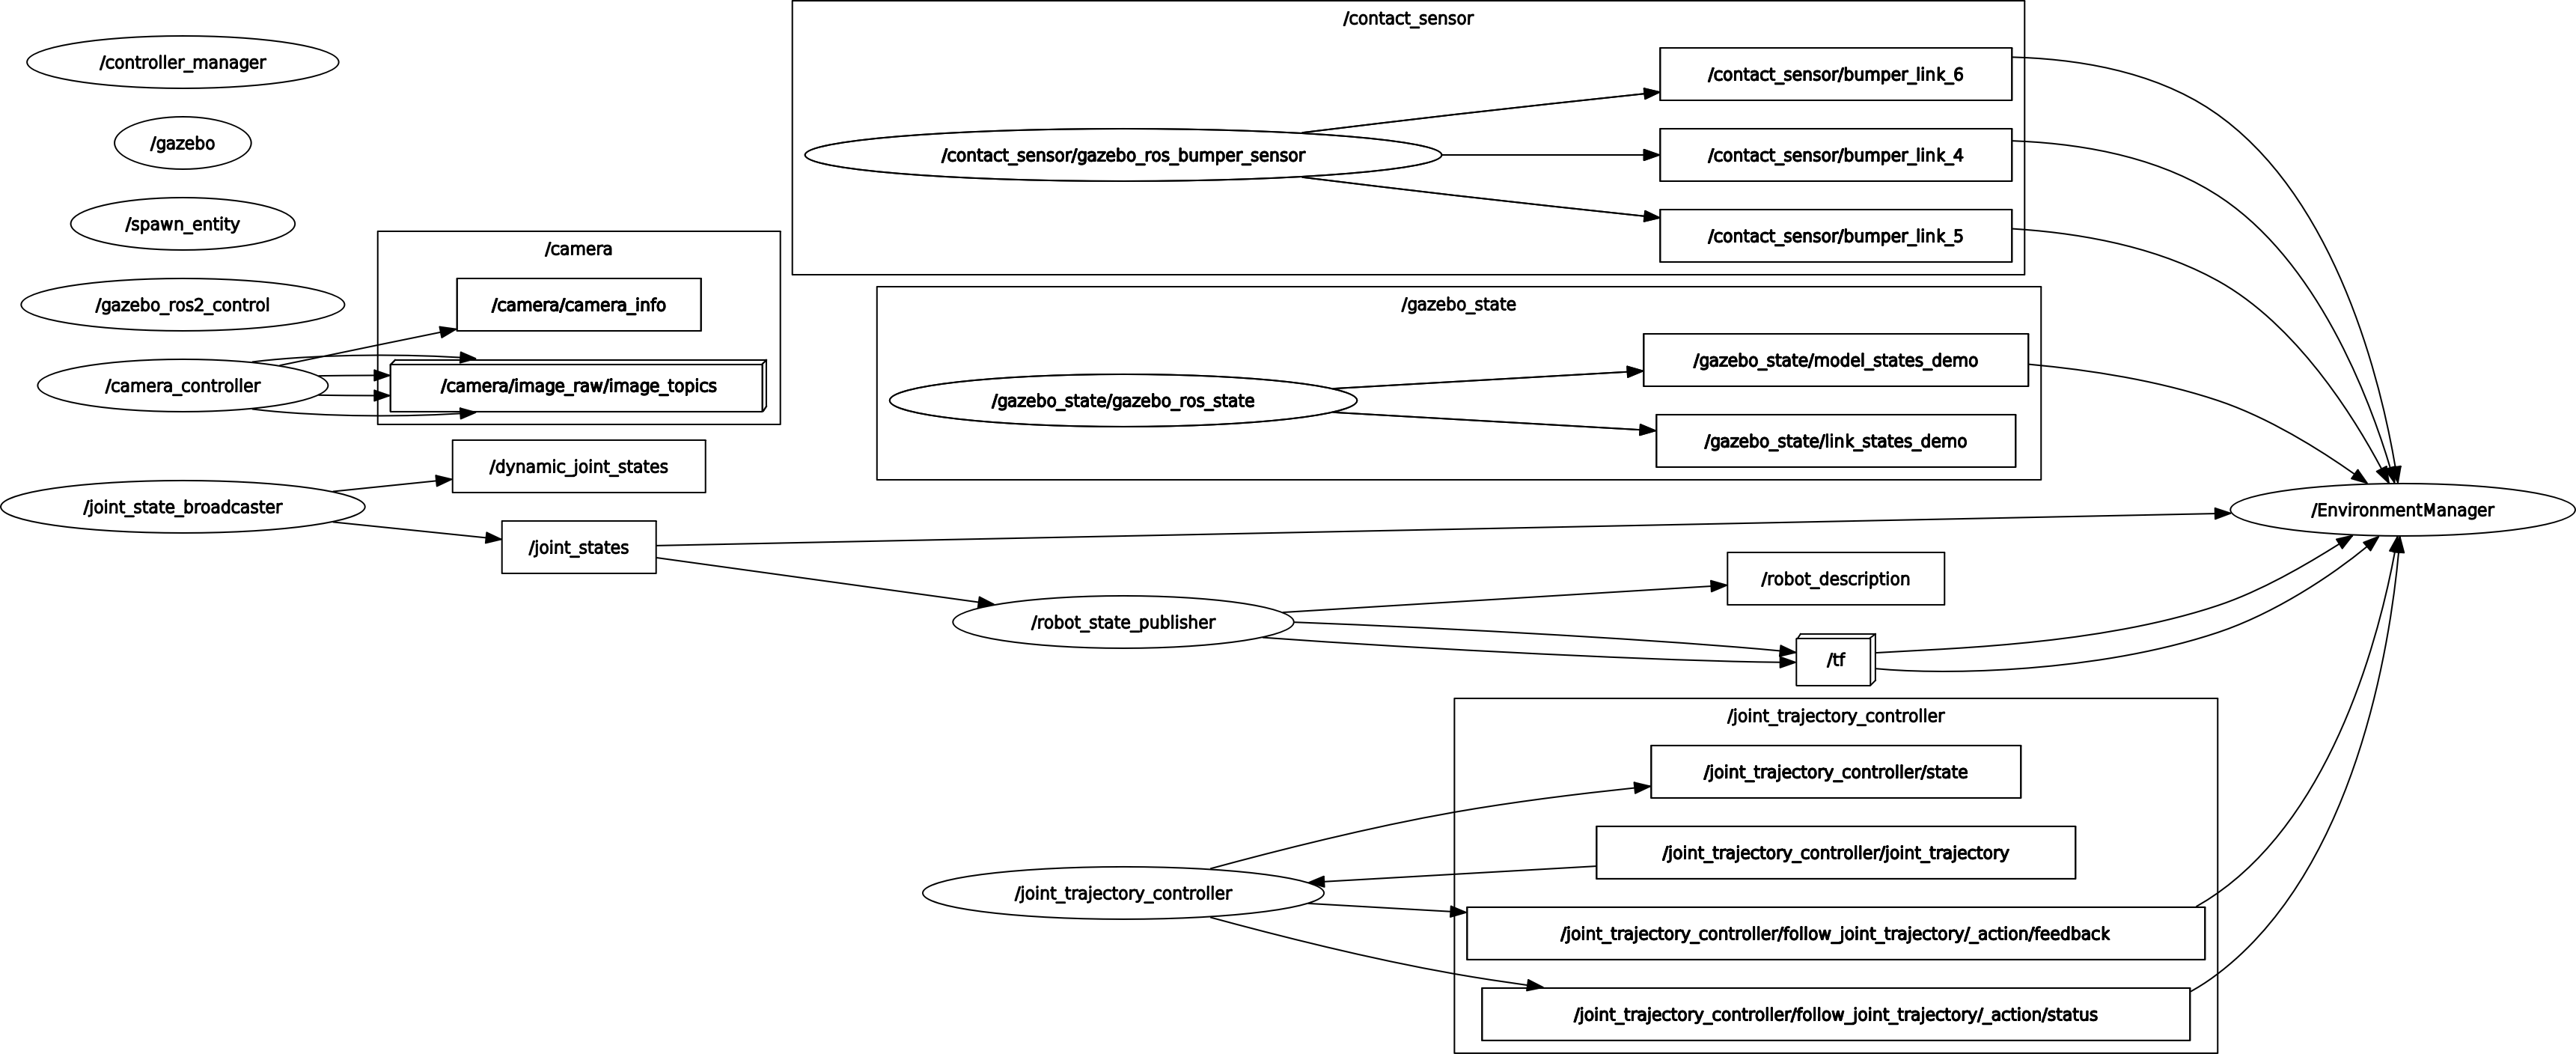
\includegraphics[width=0.99\linewidth]{rosgraph_latest}
\caption{ROS nodes and topics active when running the main program.}
\label{fig:rosgraphlatest}
\end{figure}

\subsection{Hardware and Development Environment} 

\begin{table}[H]
\centering
\begin{tabular}{ | c | c | }
\hline
\rowcolor{gray!50}
\multicolumn{2}{|c|}{\textbf{Environment Setup}} \\
\hline
\rowcolor{gray!25}
\textbf{Main Component} & \textbf{Metric} \\
\hline
Operating System & Ubuntu 20.04.3 LTS \\
\rowcolor{gray!10}
Processor & Intel(R) Core(TM) i7-4790 CPU @ 3.60GHz \\
Memory / Disk Capacity & 16GB / 500GB \\
\rowcolor{gray!10}
Graphics Card (GPU) & NVIDIA GeForce GTX 1660 Ti \\
GPU Memory (VRAM) & 6GB \\
\rowcolor{gray!10}
Robot Operating System (ROS) Version & ROS 2 Foxy \\
Gazebo Version & Gazebo multi-robot simulator, version 11.11.0 \\
\rowcolor{gray!10}
Python Version & 3.8.10 \\

\hline
\end{tabular}
\caption{Development environment setup.}
\label{table:hardware-specs}
\end{table}


%Should refer, where possible, to the preceding chapter, e.e.:
%Singular value decomposition of the matrix $\Sigma$ is conducted as explained in Sec.~\ref{sec:grundagen1} using the \textit{lapack} library (see Sec.~\ref{sec:grundlagen2}).

%For software development: what is the logic of the developed code, which of it was done by yourself? Sequence diagrams or UML are good tools here.

%Please give code snippets only if they take up less that 0.25 pages, and only if it is unavoidable. Longer snippets go to the appendix and are referenced like this: see App.~\ref{Snippet}.

\section{Experiments}\label{experiments}
\subsection{Testing the Environment}\label{experiment:testing-the-environment}
\subsubsection{Moving the Arm} \label{experiment:moving-the-arm}
The script $anglesPublisher.py$ defining the class $AnglesPublisher$ allows us to move the arm by making use of the $/joint\_trajectory\_controller/joint\_trajectory$ and specifying the joint angles in radians via command line. To collect the data in Table \ref{table:final-angles} the following was run 5 times:
\begin{tcolorbox}[]
\begin{minted}[fontsize=\scriptsize,linenos=false]{bash}
ros2 run kuka_kr_210_pkg anglesPublisher 0.5 0.5 0.5 0.5 0.5 0.5
\end{minted}
\end{tcolorbox}
After running the script specifying a target angle of 0.5 rads for all the joints, the results in Table \ref{table:final-angles} are obtained.

Making use of the values in Table \ref{table:final-angles}, a measurement of \\
$0.49999900427046 \pm 3.86729542790782 * 10^{-06} rad$ is obtained when the controller gets $0.5 rad$ as target value.
\begin{figure}[H]
  \centering
  \subfloat[Kuka Kr210 in starting position.]{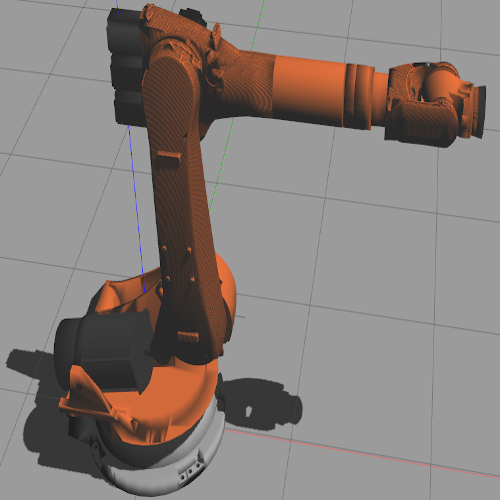
\includegraphics[width=0.6\textwidth]{kuka_start_position_new.png}\label{fig:kuka_start_position}}
  %\hfill
  \\
  \subfloat[Kuka Kr210 after moving every joint to 0.5 rads]{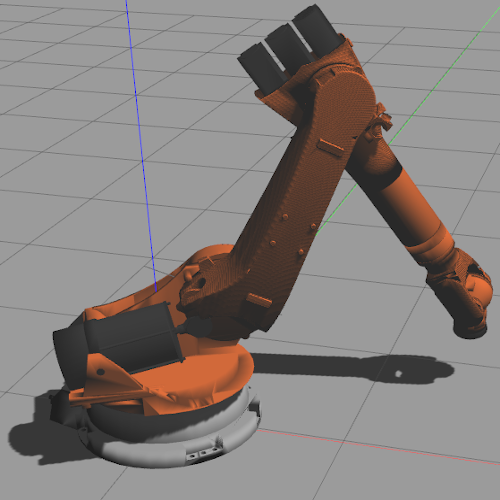
\includegraphics[width=0.6\textwidth]{kuka_end_position1_new.png}\label{fig:kuka_end_position1}}
  \caption{Robotic arm before and after publishing the target angles.}
\end{figure}

\begin{table}[H]
\centering
\begin{tabular}{c|c|c}
\hline
Real Value (Radians) & Target Value (Radians) & Difference (Radians) \\
\hline
0.499999687205044 & 0.5 & 0.000000312794956103257 \\
0.499999668258356 & 0.5 & 0.000000331741643877503 \\
0.499997756395531 & 0.5 & 0.00000224360446932081 \\
0.499999687185443 & 0.5 & 0.000000312814556535645 \\
0.499999687205041 & 0.5 & 0.000000312794958823304 \\
0.50000422755606 & 0.5 & -0.00000422755605988812 \\
0.500004208609269 & 0.5 & -0.00000420860926908517 \\
0.500002296736044 & 0.5 & -0.00000229673604401626 \\
0.50000422753646 & 0.5 & -0.00000422753645956675 \\
0.500004227556057 & 0.5 & -0.00000422755605722358 \\
0.500000658598723 & 0.5 & -0.000000658598723113357 \\
0.500000639652042 & 0.5 & -0.000000639652042444538 \\
0.499998727789975 & 0.5 & 0.00000127221002532707 \\
0.500000658579123 & 0.5 & -0.000000658579122791991 \\
0.50000065859872 & 0.5 & -0.0000006585987203378 \\
0.499992295778437 & 0.5 & 0.00000770422156293193 \\
0.499992276831646 & 0.5 & 0.00000772316835362386 \\
0.499990364958472 & 0.5 & 0.00000963504152823314 \\
0.499992295758838 & 0.5 & 0.00000770424116236512 \\
0.499992295778435 & 0.5 & 0.00000770422156470829 \\
0.50000168446693 & 0.5 & -0.00000168446693038504 \\
0.500001665520483 & 0.5 & -0.00000166552048330715 \\
0.499999753682106 & 0.5 & 0.000000246317894136983 \\
0.50000168444733 & 0.5 & -0.00000168444733006368 \\
0.500001684466927 & 0.5 & -0.00000168446692683233 \\
0.499997811745677 & 0.5 & 0.00000218825432352077 \\
0.499997792799086 & 0.5 & 0.00000220720091448356 \\
0.49999588094579 & 0.5 & 0.00000411905420971692 \\
0.499997811726076 & 0.5 & 0.00000218827392378662 \\
0.499997811745674 & 0.5 & 0.0000021882543261853 \\
\hline
\end{tabular}
\caption{Final values for the joints' angles after setting a target of 0.5 radians.}
\label{table:final-angles}
\end{table}

\subsubsection{Reading Images from the Camera Sensor}\label{experiment:reading-images}
To test if it is really possible to get images from the camera sensor, the script $cameraSubscriber.py$ was created. 
\begin{figure}[H]
  \centering
  \subfloat[Gazebo world and robotic arm at the beginning of the experiment.]{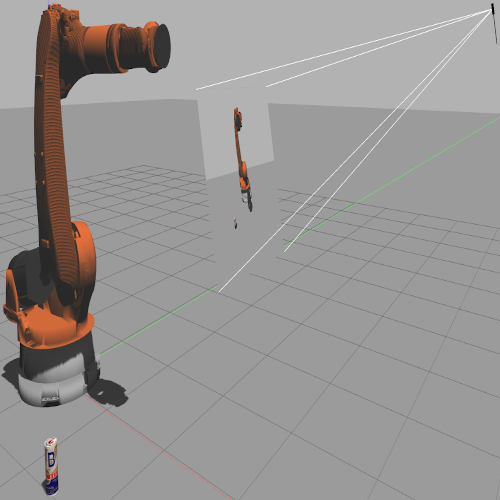
\includegraphics[width=0.49\textwidth]{kuka_camera_1_new.png}\label{fig:kuka_camera_1}}
  \hfill
  \subfloat[Image captured by the cameraSubscriber.py script before moving the arm.]{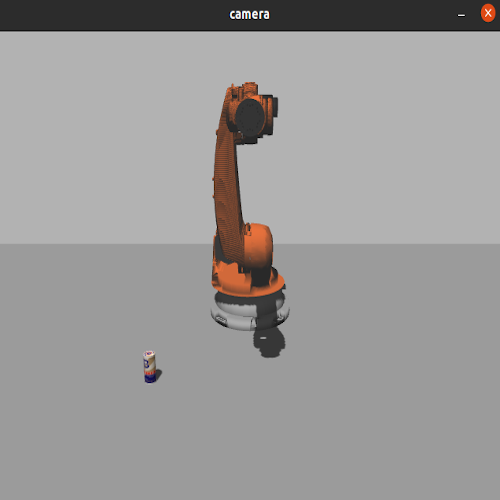
\includegraphics[width=0.49\textwidth]{kuka_camera_2_new.png}\label{fig:kuka_camera_2}}
  \caption{Image of the gazebo world and from the camera sensor at starting position.}
\end{figure}

\begin{figure}[H]
  \centering
  \subfloat[Gazebo world and robotic arm position after executing a moving command.]{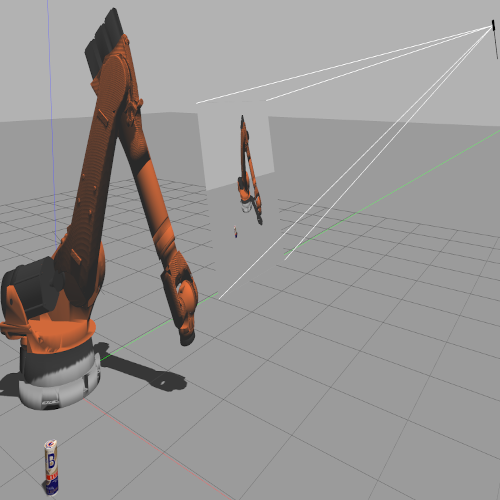
\includegraphics[width=0.49\textwidth]{kuka_camera_3_new.png}\label{fig:kuka_camera_3}}
  \hfill
  \subfloat[Image captured by the cameraSubscriber.py script after moving the arm.]{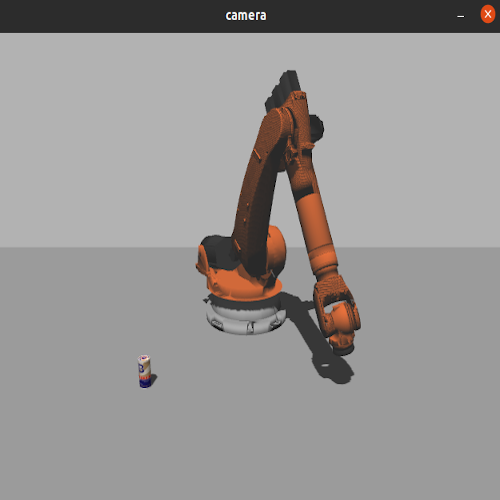
\includegraphics[width=0.49\textwidth]{kuka_camera_4_new.png}\label{fig:kuka_camera_4}}
  \caption{Image of the gazebo world and from the camera sensor after moving the arm.}
\end{figure}

The $cameraSubscriber.py$ subscribes to the $/camera/image\_raw$ and as Figures \ref{fig:kuka_camera_2} and \ref{fig:kuka_camera_4} show, the script can obtain the images and in this case just shows them in a new window.

\subsubsection{Detecting Collisions}\label{experiment:detecting-collisions}
In this experiment the script $anglesPublisher.py$ is used to move the arm to touch the object (a can). While doing this the topics $/contact\_sensor/bumper\_link\_4$, \\ $/contact\_sensor/bumper\_link\_5$, and $/contact\_sensor/bumper\_link\_6$ are monitored using Rqt \ref{rviz_rqt} so collisions between the beer can and Links 4, 5, or 6 can be detected.
After moving the arm to make the collision happen between the can and Link 6 of the arm as in Figure \ref{fig:rqtlink6collision}, it can be seen in Figure \ref{fig:rqtlink6collision} that for the topic $/contact\_sensor/bumper\_link\_6$ there is a message of type $ContactState$ in $states$ which indicates that the collisions sensor is working properly and we can rely on them in future experiments.

\begin{figure}[H]
\centering
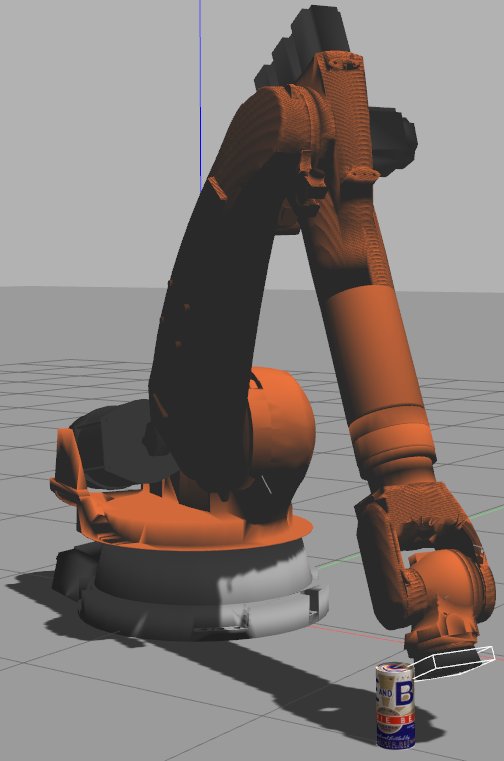
\includegraphics[width=0.4\linewidth]{link_6_collision}
\caption{Collision between the can and Link 6 or end effector of the arm.}
\label{fig:link6collision}
\end{figure}
\begin{figure}[H]
\centering
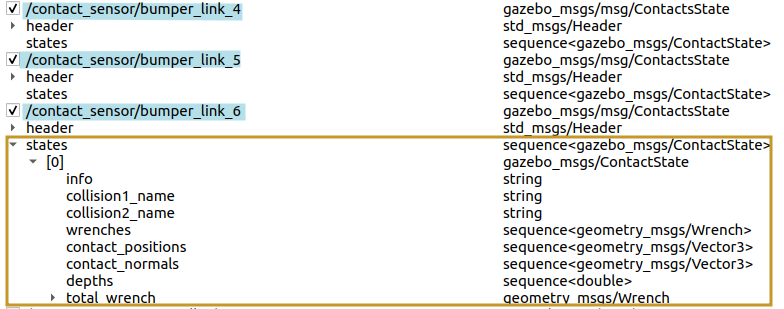
\includegraphics[width=0.9\linewidth]{rqt_link_6_collision}
\caption[Contact sensors monitoring with Rqt.]{Monitoring the topics \textit{/contact\_sensor/bumper\_link\_4}, \\ \textit{ /contact\_sensor/bumper\_link\_5}, and \textit{/contact\_sensor/bumper\_link\_6} in Rqt \ref{rviz_rqt}. The first column is the name of the topics, and the second is the type of message they handle. }
\label{fig:rqtlink6collision}
\end{figure}

\subsection{Learning to touch the object}\label{experiment:learning-touch-object}
\subsubsection{Experiment 1}\label{experiment:experiment-1}
In this experiment the Main Program \ref{main-program} was run with the parameters in Table \ref{tab:hyperparams-exp-1}. The experiment consists in finding out if the arm can learn to touch the can.
\begin{table}[h]
\centering
\begin{tabular}{l l}
\hline
Parameter & Value \\
\hline
Discount Factor ($\gamma$) & 0.99 \\
Batch Size & 512 \\
Epsilon Start Value & 1 \\
Epsilon Final & 0.01 \\
Epsilon Decay Rate & 0.0001 \\
Episodes before updating the Target Network & 10 \\
Replay Memory size & 10240 \\
Learning Rate & 0.001 \\
Number of Episodes & 50 \\
Maximum Steps per episode & 500 \\
\hline
\end{tabular}
\caption{Hyperparameters values for the reinforcement learning algorithm in Experiment 1.}
\label{tab:hyperparams-exp-1}
\end{table}

As the results in Figure \ref{fig:rewards_episodes_50_gamma_099} show, the arm learns to get a reward of over $125$ consistently from episode $25$. Also in Figure \ref{fig:nSteps_episodes_50_gamma_099} can be seen that the number of steps per episode stay around or below $100$. This means that the arm learns to touch the object.

\begin{figure}[H]
  \centering
  \subfloat[Sum of rewards in an episode or episode reward per episode]
  {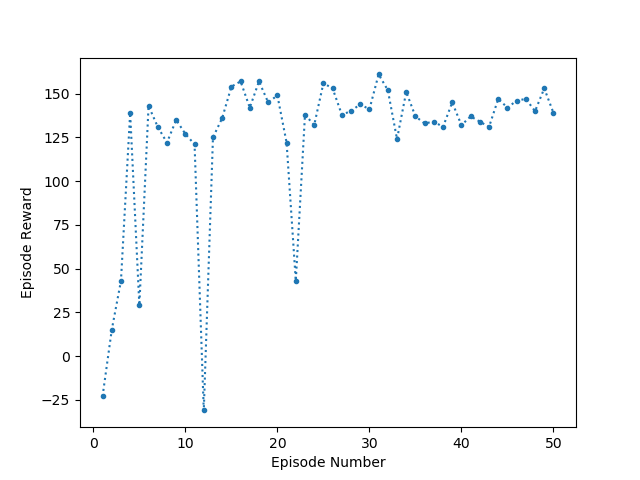
\includegraphics[width=0.49\textwidth]{rewards_episodes_50_gamma_099.png}\label{fig:rewards_episodes_50_gamma_099}}
  \hspace{0\textwidth}  
  \subfloat[Number of steps per episode.]
  {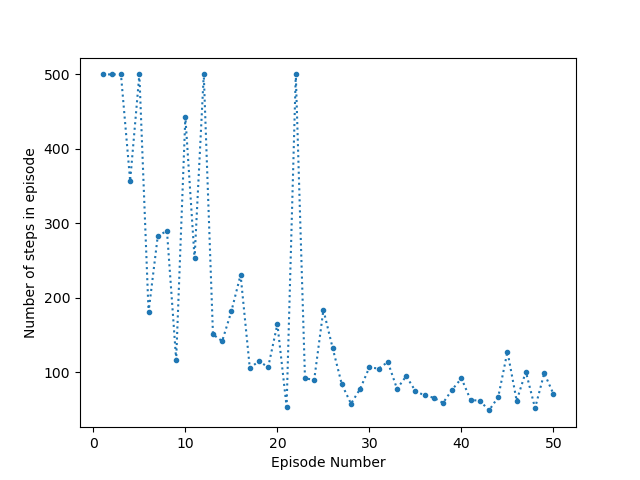
\includegraphics[width=0.49\textwidth]{nSteps_episodes_50_gamma_099.png}\label{fig:nSteps_episodes_50_gamma_099}}
  \caption{Reward per episode and number of steps per episode for experiment 1 with parameters in Table \ref{tab:hyperparams-exp-1}.}
  \label{fig:experiment-1}
\end{figure}
\subsubsection{Experiment 2}\label{experiment:experiment-2}
This experiment is similar to Experiment 1, just the number of episodes changes to 100 to see if the learning of the arm can be improved.
\begin{table}[H]
\centering
\begin{tabular}{l l}
\hline
Parameter & Value \\
\hline
Discount Factor ($\gamma$) & 0.99 \\
Batch Size & 512 \\
Epsilon Start Value & 1 \\
Epsilon Final & 0.01 \\
Epsilon Decay Rate & 0.0001 \\
Episodes before updating the Target Network & 10 \\
Replay Memory size & 10240 \\
Learning Rate & 0.001 \\
Number of Episodes & 100 \\
Maximum Steps per episode & 500 \\
\hline
\end{tabular}
\caption{Hyperparameters values for the reinforcement learning algorithm in Experiment 2.}
\label{tab:hyperparams-exp-2}
\end{table}

\begin{figure}[H]
\centering
\sbox{\measurebox}{%
  \begin{minipage}[b]{.47\textwidth}
  \subfloat
    [Collision between Link 6 of the robotic arm and can at the end of Experiment 2.]
    {\label{fig:kuka_collision_100_episodes}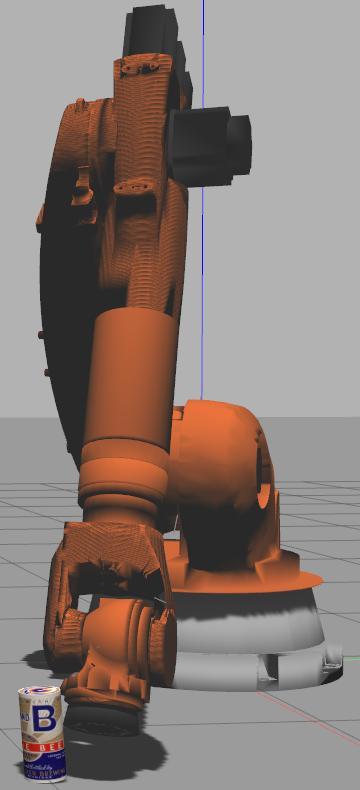
\includegraphics[width=\textwidth,height=15cm]{kuka_collision_100_episodes}}
  \end{minipage}}
\usebox{\measurebox}\qquad
\begin{minipage}[b]{.47\textwidth}
\centering
\subfloat
  [Sum of rewards in an episode or episode reward per Episode]
  {\label{fig:rewards_episodes_100_gamma_099}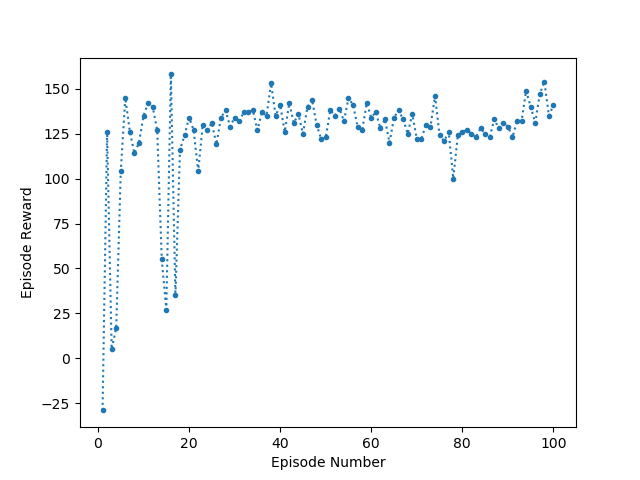
\includegraphics[width=\textwidth,height=7.3cm]{rewards_episodes_100_gamma_099}} \\
\subfloat
  [Number of steps per episode.]
  {\label{fig:nSteps_episodes_100_gamma_099}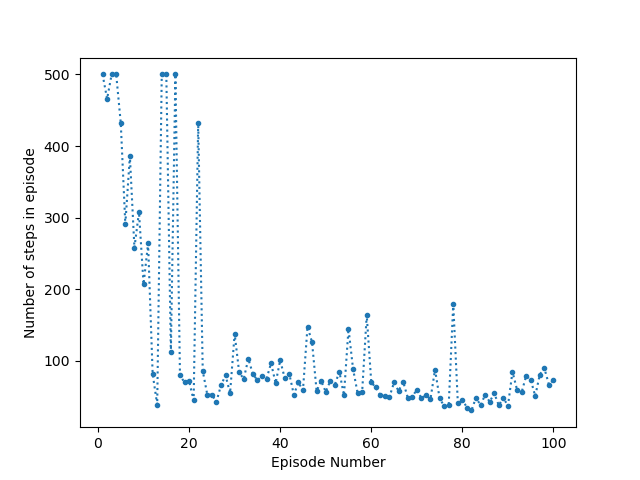
\includegraphics[width=\textwidth,height=7.3cm]{nSteps_episodes_100_gamma_099}}
\end{minipage}
\caption{Collision of the robotic arm and the can and Experiment 2 results.}
\label{fig:experiment-2}
\end{figure}

\subsubsection{Experiment 3}\label{experiment:experiment-3}
This experiment was run using the parameters in Table \ref{tab:hyperparams-exp-3}
\begin{table}[H]
\centering
\begin{tabular}{l l}
\hline
Parameter & Value \\
\hline
Discount Factor ($\gamma$) & 0.5 \\
Batch Size & 512 \\
Epsilon Start Value & 1 \\
Epsilon Final & 0.01 \\
Epsilon Decay Rate & 0.0001 \\
Episodes before updating the Target Network & 10 \\
Replay Memory size & 10240 \\
Learning Rate & 0.001 \\
Number of Episodes & 100 \\
Maximum Steps per episode & 500 \\
\hline
\end{tabular}
\caption{Hyperparameters values for the reinforcement learning algorithm in Experiment 3.}
\label{tab:hyperparams-exp-3}
\end{table}
In addition to the total reward per episode and number of steps per episode, the exploration rate ($\epsilon$) was also monitored in this experiment as can be seen in Figure \ref{fig:epsilon_episodes_100_gamma_05}.
\begin{figure}[H]
\centering
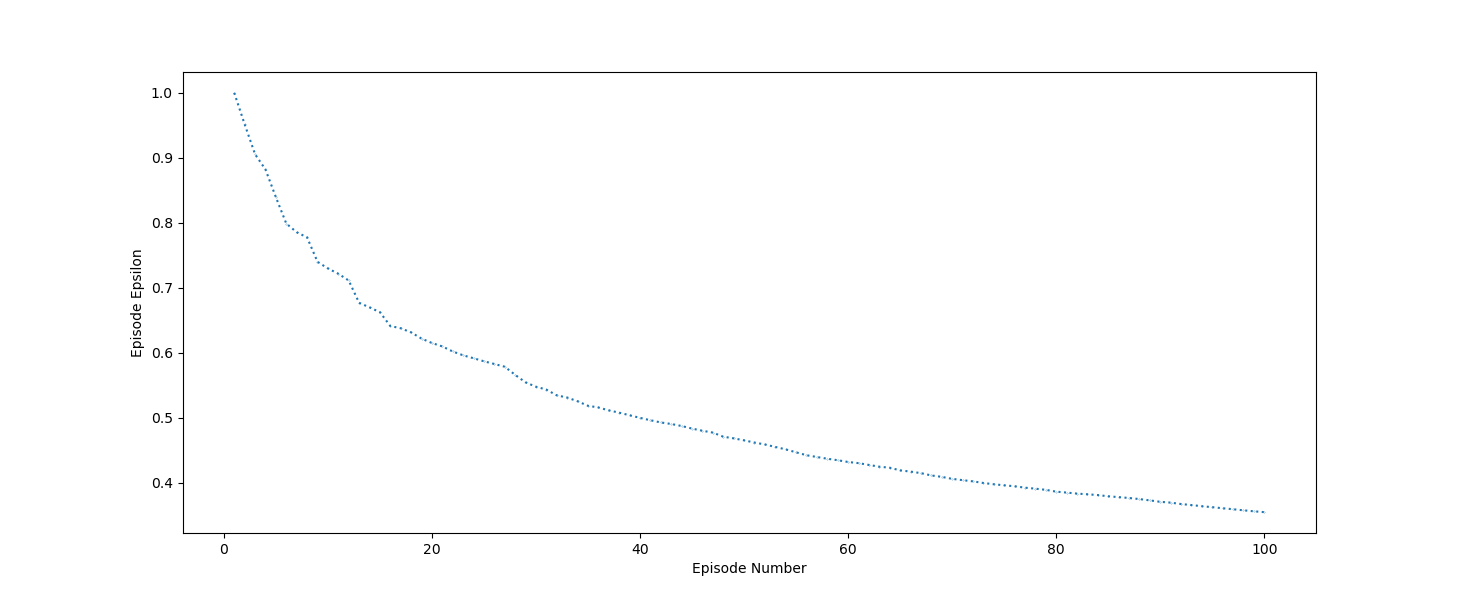
\includegraphics[width=0.9\linewidth]{epsilon_episodes_100_gamma_05.png}
\caption{Exploration rate ($\epsilon$) value at the beginning of each episode. }
\label{fig:epsilon_episodes_100_gamma_05}
\end{figure}


\begin{figure}[H]
\centering
\sbox{\measurebox}{%
  \begin{minipage}[b]{.47\textwidth}
  \subfloat
    [Collision between Link 6 of the robotic arm and can at the end of Experiment 3.]
    {\label{fig:kuka_collision_100_episodes_gamma_05}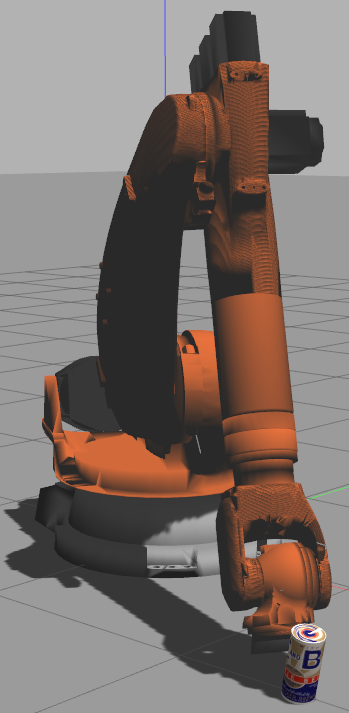
\includegraphics[width=\textwidth,height=15cm]{kuka_collision_100_episodes_gamma_05.png}}
  \end{minipage}}
\usebox{\measurebox}\qquad
\begin{minipage}[b]{.47\textwidth}
\centering
\subfloat
  [Sum of rewards in an episode or episode reward per episode]
  {\label{fig:rewards_episodes_100_gamma_05}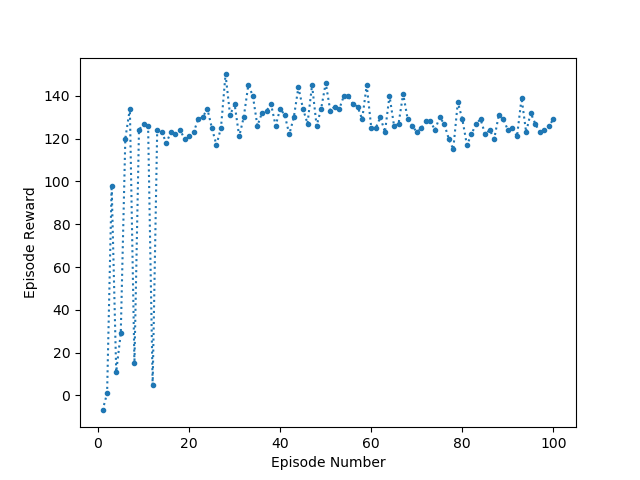
\includegraphics[width=\textwidth,height=7.3cm]{rewards_episodes_100_gamma_05}} \\
\subfloat
  [Number of steps per episode.]
  {\label{fig:nSteps_episodes_100_gamma_05}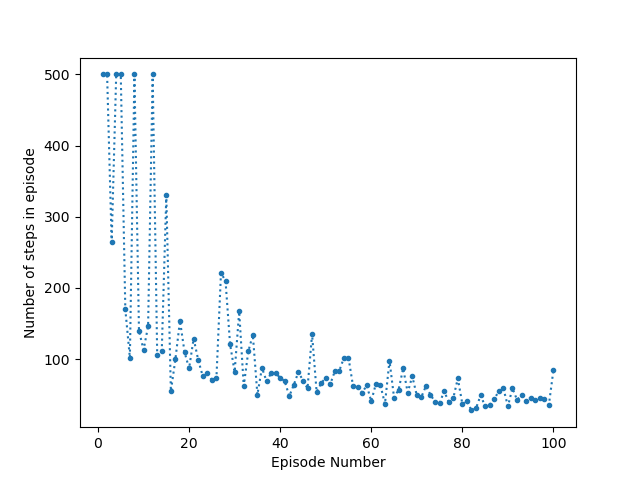
\includegraphics[width=\textwidth,height=7.3cm]{nSteps_episodes_100_gamma_05}}
\end{minipage}
\caption{Collision of the robotic arm and the can and Experiment 3 results.}
\label{fig:experiment-3}
\end{figure}

\subsubsection{Experiment 4}\label{experiment:experiment-4}
The experiment was run with parameters in Table \ref{tab:hyperparams-exp-4}.
\begin{table}[H]
\centering
\begin{tabular}{l l}
\hline
Parameter & Value \\
\hline
Discount Factor ($\gamma$) & 0.5 \\
Batch Size & 2048 \\
Epsilon Start Value & 1 \\
Epsilon Final & 0.01 \\
Epsilon Decay Rate & 0.00001 \\
Episodes before updating the Target Network & 5 \\
Replay Memory size & 10240 \\
Learning Rate & 0.001 \\
Number of Episodes & 300 \\
Maximum Steps per episode & 500 \\
\hline
\end{tabular}
\caption{Hyperparameters values for the reinforcement learning algorithm in Experiment 4.}
\label{tab:hyperparams-exp-4}
\end{table}
The exploration rate at the beginning of each episode is shown in Figure \ref{fig:epsilon_episodes_300_gamma_05}
\begin{figure}[H]
\centering
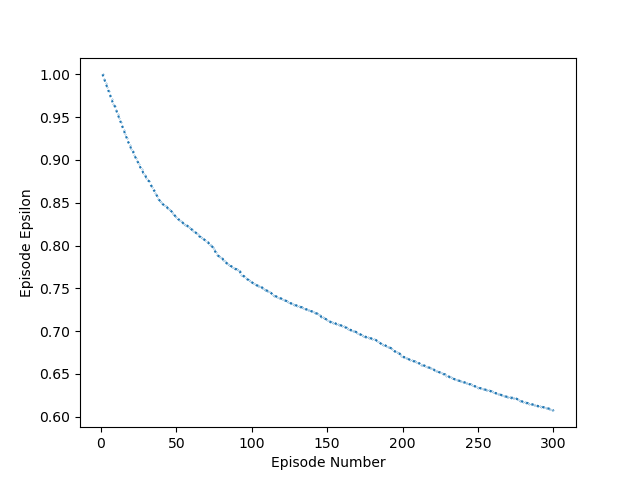
\includegraphics[width=0.9\linewidth]{epsilon_episodes_300_gamma_05.png}
\caption{Exploration rate ($\epsilon$) value at the beginning of each episode. }
\label{fig:epsilon_episodes_300_gamma_05}
\end{figure}

\begin{figure}[H]
\centering
\sbox{\measurebox}{%
  \begin{minipage}[b]{.3\textwidth}
  \subfloat
    [Collision between Link 6 of the robotic arm and can at the end of Experiment 4.]
    {\label{fig:kuka_collision_300_episodes_gamma_05}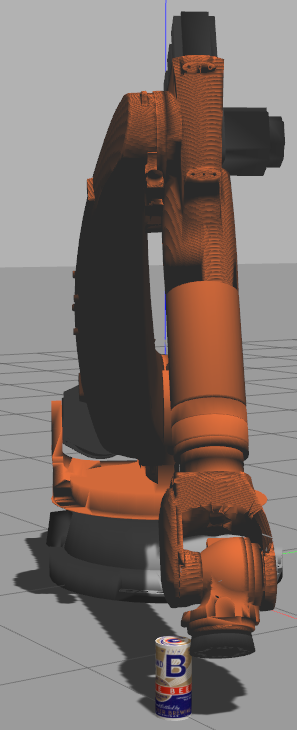
\includegraphics[width=\textwidth,height=15cm]{kuka_collision_300_episodes_gamma_05.png}}
  \end{minipage}}
\usebox{\measurebox}\qquad
\begin{minipage}[b]{.64\textwidth}
\centering
\subfloat
  [Sum of rewards in an episode or episode reward per episode]
  {\label{fig:rewards_episodes_300_gamma_05}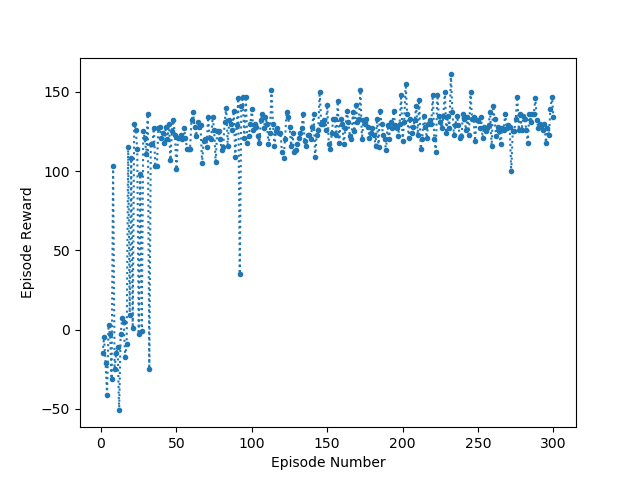
\includegraphics[width=\textwidth,height=7.3cm]{rewards_episodes_300_gamma_05}} \\
\subfloat
  [Number of steps per episode.]
  {\label{fig:nSteps_episodes_300_gamma_05}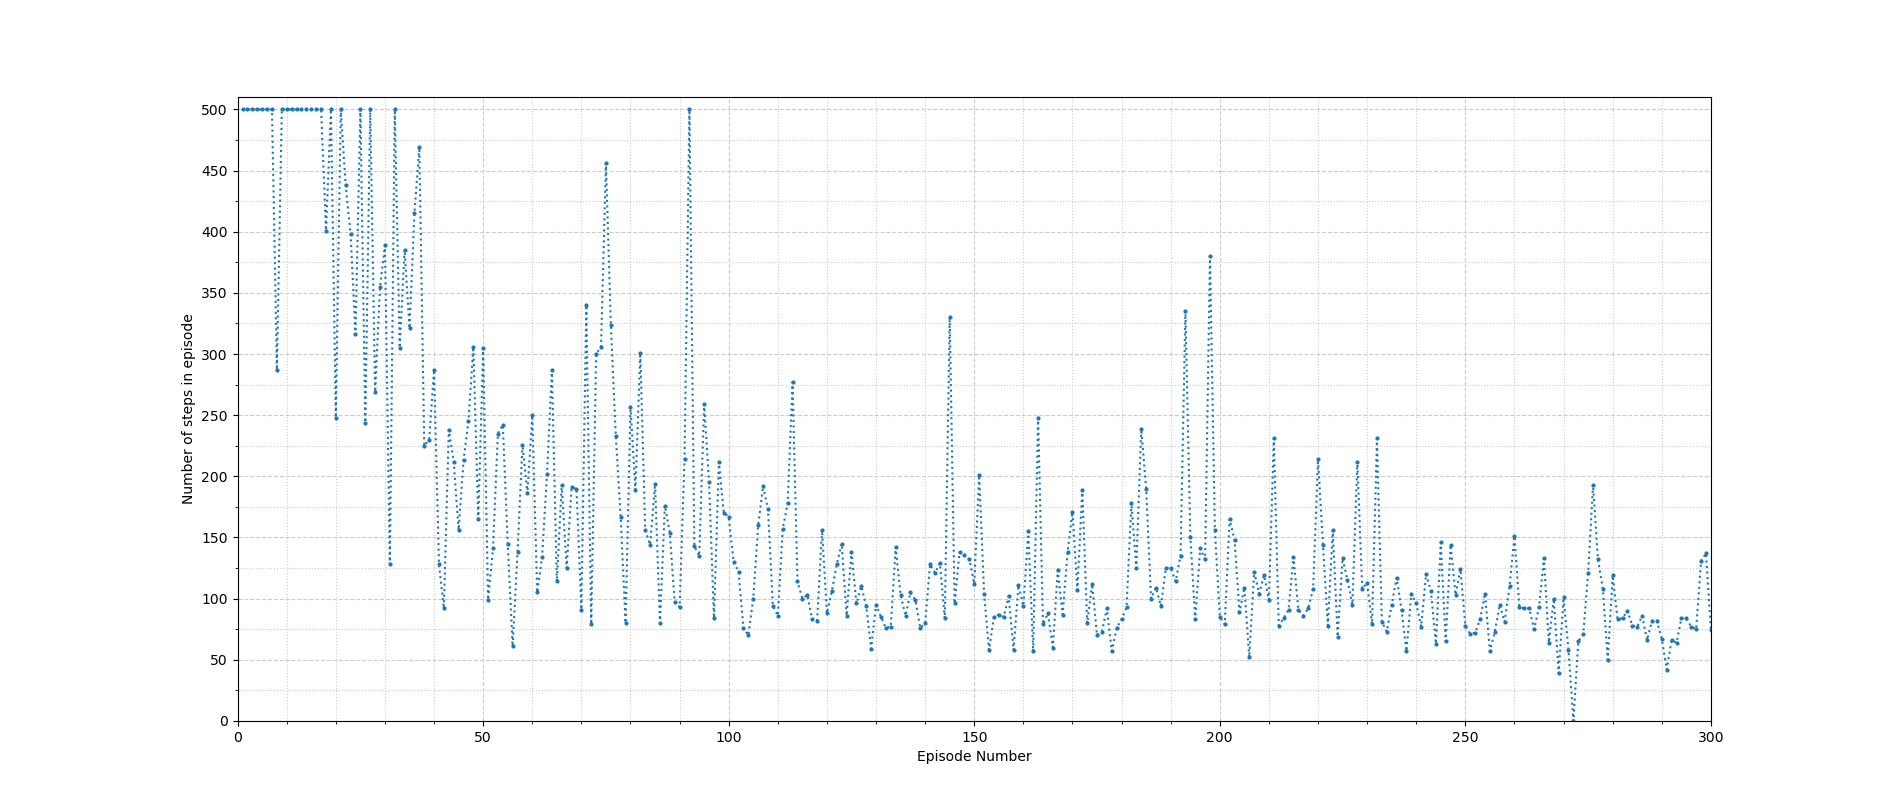
\includegraphics[width=\textwidth,height=7.3cm]{nSteps_episodes_300_gamma_05}}
\end{minipage}
\caption{Collision of the robotic arm and the can and Experiment 4 results.}
\label{fig:experiment-4}
\end{figure}

\subsubsection{Experiment 5}\label{experiment:experiment-5}
The experiment was run with parameters in Table \ref{tab:hyperparams-exp-5}.
\begin{table}[H]
\centering
\begin{tabular}{l l}
\hline
Parameter & Value \\
\hline
Discount Factor ($\gamma$) & 0.5 \\
Batch Size & 8184 \\
Epsilon Start Value & 1 \\
Epsilon Final & 0.01 \\
Epsilon Decay Rate & 0.00002 \\
Episodes before updating the Target Network & 5 \\
Replay Memory size & 102400 \\
Learning Rate & 0.001 \\
Number of Episodes & 800 \\
Maximum Steps per episode & 500 \\
\hline
\end{tabular}
\caption{Hyperparameters values for the reinforcement learning algorithm in Experiment 5.}
\label{tab:hyperparams-exp-5}
\end{table}
The experiment results can be seen in Figure \ref{fig:experiment-5}.
\begin{figure}[H]
  \centering
  \subfloat[Sum of rewards in an episode or episode reward per episode.]{\label{fig:rewards_episodes_800_gamma_05}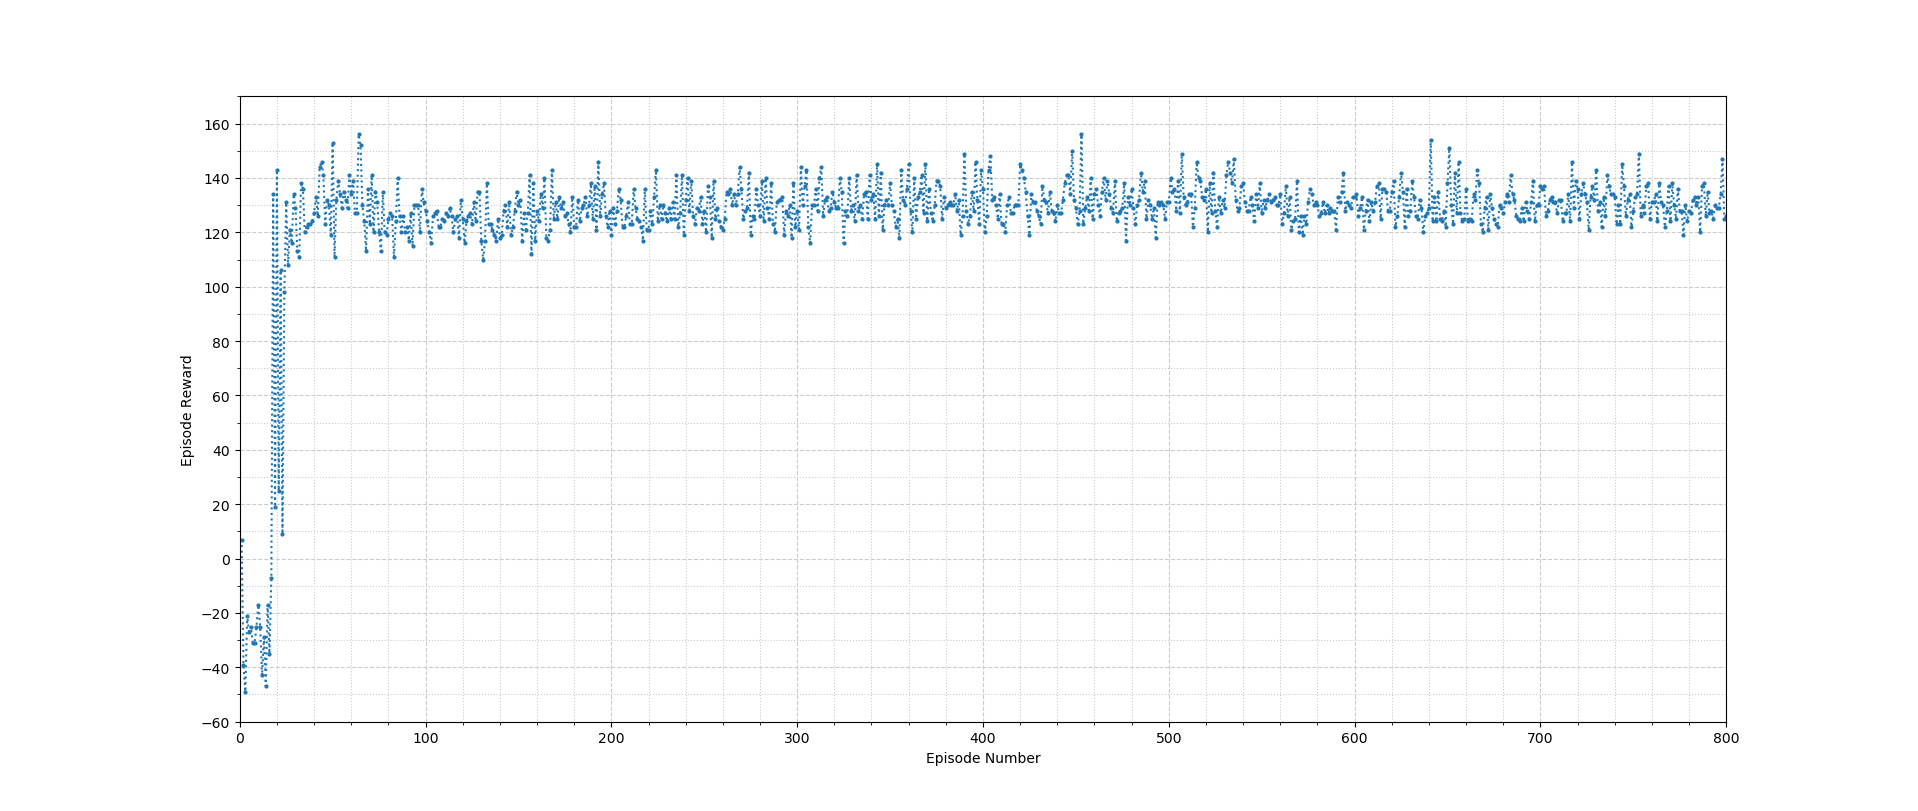
\includegraphics[width=0.99\textwidth]{rewards_episodes_800_gamma_05.png}}\\
  \subfloat[Number of steps per episode.]{\label{fig:nSteps_episodes_800_gamma_05}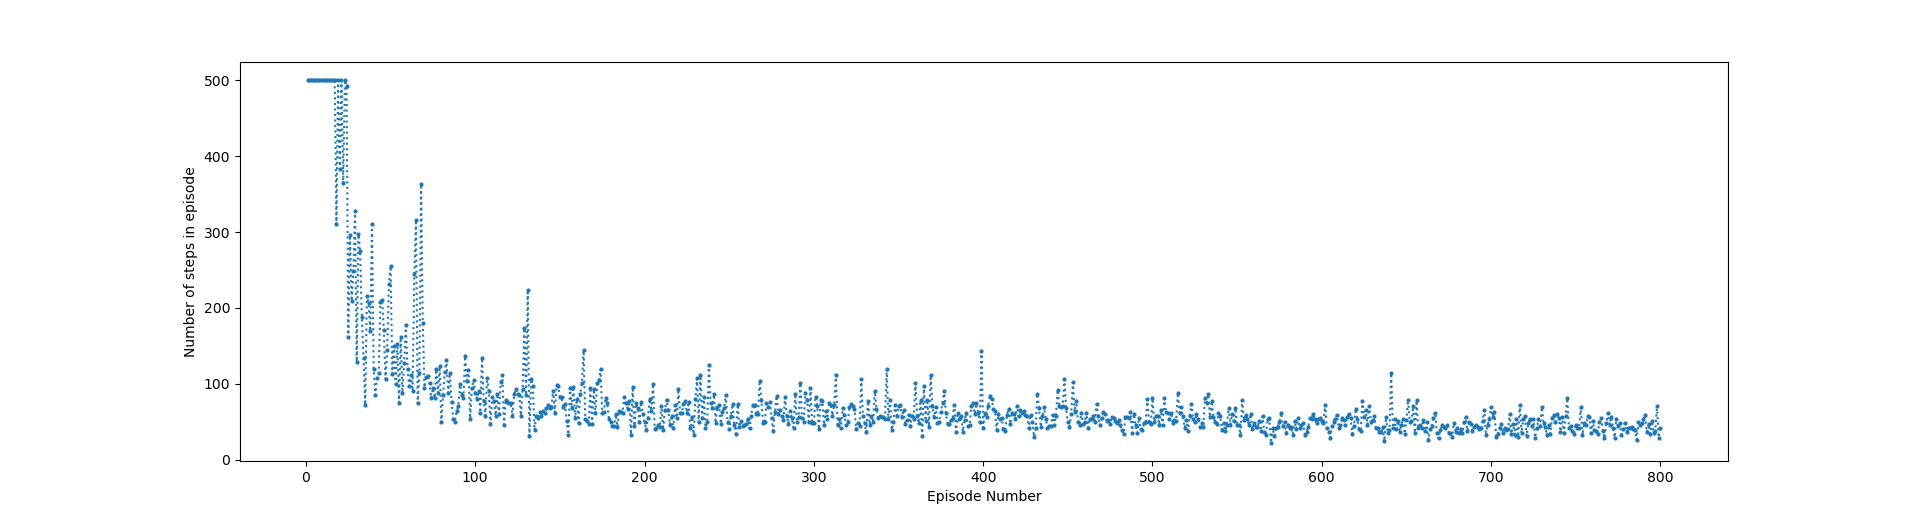
\includegraphics[width=0.99\textwidth]{nSteps_episodes_800_gamma_05.png}} \\
  \subfloat[Exploration rate ($\epsilon$) value at the beginning of each episode.]{\label{fig:epsilon_episodes_800_gamma_05}\includegraphics[width=0.99\textwidth]{epsilon_episodes_800_gamma_05.png}}
  \caption{Results for Experiment 5.}
  \label{fig:experiment-5}
\end{figure}

%\par\noindent\rule{\textwidth}{0.4pt}
%Show here that the goals from the introduction were achieved (or not achieved), you need at least one experiment per goal. Use screenshots, diagrams, plots, photos, etc. as necessary.

\section{Discussion}
In this thesis, we explored the use of a DQN to train a robotic arm to learn to touch an object. Our experiments were performed on a simulated robotic arm in a virtual environment as in \ref{sec:env-preparation}.
The results from the experiments \ref{experiment:moving-the-arm}, \ref{experiment:reading-images}, and \ref{experiment:detecting-collisions} show that the robotic arm simulation was successfully implemented. Furthermore, it is possible to interact with the simulation programmatically, treating it as a Markov Decision Process. experiment \ref{experiment:moving-the-arm} shows that we can rely on the used ROS 2 packages to control the position of the arm with an accuracy in the order of $10^{-06} rad$.
Also experiment \ref{experiment:reading-images} creates new possibilities for future studies as the images from the camera sensor could be used instead of the built in Gazebo and ROS plugins to know the position of the objects in the simulated world, making easier the transition from the simulation to the real world because it is easier to work with a camera instead of location sensors in the end effector of the arm and in the can; in fact, the idea of adding a sensor to the can in the real world is a little troublesome because ideally we should be able to just place any object in our world without having to alter it in any way. 
In addition, experiment \ref{experiment:detecting-collisions} proves that it is possible to use contact sensors in the simulation and perform actions based on the readings from this sensors. Thus, it safe to claim that experiments in \ref{experiment:testing-the-environment} really represent a fully working simulation of a robotic arm in which not only Markov Decision Processes can be implemented, but also Reinforcement Learning algorithms can be run. In fact, experiments in \ref{experiment:learning-touch-object} show that it is possible. For example, in experiment 1, in \ref{experiment:experiment-1} in Figure \ref{fig:experiment-1} it can be seen that the arm consistently achieves higher rewards and finishes the episodes in less iterations as the simulation goes on, this proves that the arm learns about the environment and in time finds the can and learns to touch it. However, to know if the arm can learn a better way to touch the arm, experiment 2 in \ref{experiment:experiment-2} is run. Here, we just let the experiment run $50$ more steps compared to Experiment 1 in \ref{experiment:experiment-1}. As can be seen in Figure \ref{fig:rewards_episodes_100_gamma_099} in the last steps of the process, the total rewards does not significantly improves compared Figure \ref{fig:rewards_episodes_50_gamma_099}, neither does the number of steps the arm needs to touch the can when we compare Figures \ref{fig:nSteps_episodes_50_gamma_099} and \ref{fig:nSteps_episodes_100_gamma_099}. The goals in \ref{sec:goals} have been so far achieved as we have a working simulation of a robotic arm working, the simulated robotic arm learns to touch the can in the simulated world (Figure \ref{fig:kuka_collision_100_episodes}). Next let us examine if this can be improved and how the exploration-exploitation trade off is being dealt with. 

Experiment 3 in \ref{experiment:experiment-3} examines the learning process with a discount factor of $\gamma = 0.5$ instead of a $\gamma = 0.99$ as in the previous experiments. The idea is to see if the learning process improves or gets worse. When comparing Figure \ref{fig:kuka_collision_100_episodes} and Figure \ref{fig:kuka_collision_100_episodes_gamma_05} we can see that even though the arm touches the can from different positions, it does learn to touch it. Moreover, by comparing Figures \ref{fig:rewards_episodes_100_gamma_05}, \ref{fig:nSteps_episodes_100_gamma_05} to Figures  \ref{fig:rewards_episodes_100_gamma_099}, \ref{fig:nSteps_episodes_100_gamma_099} we can see that the learning process is neither better or worse. On the other hand, Figure \ref{fig:epsilon_episodes_100_gamma_05} shows that during the whole performance there was some randomness due te the explore-exploit trade-off therefore there were always random actions in every episode.

Experiment 4 in \ref{experiment:experiment-4} is an attempt to improve results i.e. obtaining higher rewards and finish the episode in fewer steps. To try this, the Batch size is increased to $2048$, the Decay rate for epsilon $\epsilon$ is reduced to $0.00001$, and the number of episodes is increased to $300$. With this parameters as can be seen in Figure \ref{fig:experiment-4}, the total rewards per episode in Figure \ref{fig:rewards_episodes_300_gamma_05} are not significantly better as the ones in Figure \ref{fig:rewards_episodes_100_gamma_05} since in both cases, they hover around a total reward value of $150$. But as can be seen in Figure \ref{fig:epsilon_episodes_100_gamma_05} the exploration rate in Experiment 4 was always above $0.6$ compared to the exploration rate in Figure \ref{fig:epsilon_episodes_100_gamma_05} in Experiment 3 which gets to values lower than $0.4$. It is important to note that with higher exploration rates, more random actions take place and this random actions make the episode longer as the action does not necessarily aim to get the arm closer to the can. 

Experiment 5 in \ref{experiment:experiment-5} is designed to compare the total rewards and iterations per episodes with parameters that would let the simulation run for more time steps and consider more experiences when training the neural network. With the number of steps per episode set to $800$, a higher batch size of $8184$ and a decay rate for epsilon of $0.00002$ it is possible to see total rewards of the robotic arm at exploration rates (Figure \ref{fig:epsilon_episodes_800_gamma_05}) that have similar values as those in Figure \ref{fig:epsilon_episodes_100_gamma_05}. Comparing the total rewards in Figures \ref{fig:rewards_episodes_300_gamma_05} and \ref{fig:rewards_episodes_800_gamma_05} it can be seen that the performance is not significantly different as the total reward still hovers between $120$ and $140$, and the number of steps per episode in Figure \ref{fig:nSteps_episodes_300_gamma_05} is around $75$ whereas in Figure \ref{fig:nSteps_episodes_800_gamma_05} it consistenly stays below $50$ from episode $500$. Therefore, even though the total rewards per episode are similar, the steps the agent takes to complete the episodes are less which means the arm learns more efficient set of movements to touch the can in Experiment 5 \ref{experiment:experiment-5} than in previous experiments.

Our results show that the DQN approach was successful in training the robotic arm to complete the task of touching an object. The agent was able to learn a funtional policy over time and consistently achieve the desired objective. The performance of the trained agent was evaluated using two metrics: the total reward per episode and the number of episodes it took to reach the goal. The total reward per episode of the agent increased steadily during training and stabilized after approximately $200$ steps in experiments \ref{experiment:experiment-4} and \ref{experiment:experiment-5}. The number of steps to complete an episode also decreased during training, indicating that the agent was learning to perform the task more efficiently.

Several experiments were also conducted to analyze the impact of different hyperparameters on the performance of the DQN agent. Our findings suggest that the choice of hyperparameters, such as the discount factor, can affect the training. Additionally, increasing the size of the replay memory  improved the performance of the agent.

One of the limitations of our study is that it was performed on a simulated robotic arm. The transferability of the learned policy to a physical robotic arm in the real world is an important aspect to consider in future work. Another limitation is the relatively simple task of just touching an object. Future work can investigate the use of DQN for more complex tasks, such as manipulation of objects in cluttered environments.

In conclusion, the application of DQN to train a robotic arm to perform a specific task shows promising results. Our experiments demonstrate the effectiveness of this approach and provide insights into the impact of different hyperparameters on the training process. The results of this study can contribute to the development of more advanced reinforcement learning algorithms for robotics.


%2-3 pages are a good idea here. Picks up goals from the introduction (see \ref{sec:ziele}) and experiments (see \ref{sec:exp}) and explains what was achieved and what was not (and why not in this case). Compares results with results from related work, see Sec.~\ref{sec:relwork}. Draws a preliminary conclusion for the whole thesis.
%\begin{tcolorbox}\label{box:mybox}%[label=mybox]
%\begin{minted}[fontsize=\scriptsize]{python}
%action = agent.selectAction(state, policyNetwork)
%reward = environment.takeAction(action)
%nextState = environment.getState()
%print("hi")
%\end{minted}
%\end{tcolorbox}
%
%As we can see in box \ref{box:mybox}, ...
\section{Conclusion}
This thesis explored the application of the Double Q-Learning algorithm to a simulated robotic arm in a reinforcement learning setting. The theoretical foundation of the algorithm was introduced, implemented, and applied to a simple task using the Gazebo simulator and ROS 2 libraries. The experimental results show that the Double Q-Learning algorithm works as the simulated arm learns to touch the can. This work contributes to the development of reinforcement learning algorithms for training robotic arms and provides not only a robust and efficient approach but also an alternative to solving complex tasks in the robotics area.

In the experiments, a simple task for the robotic arm to perform was designed, this task consists in moving the robotic arm to a given target location so it touches an object (a can). The robotic arm had six degrees of freedom; out which only three were manipulated in the experiments. The task required a combination of forward and backward movements of this joints. The state space was given by the three joint angles and the distance between the robotic arm and the can; whereas the action space was discrete and given by the combination of possible variations for the angles. The robotic arm was trained using the Double Q-Learning algorithm.

Future work can explore the application of the algorithm to more complex tasks and environments as there are several possible avenues for future research in the field of reinforcement learning, DQN, and robotic arms. One possible direction is to explore the use the prioritized experience replay method, to improve the performance and stability of the robotic arm. Additionally, incorporating more complex reward functions, such as those that incorporate task completion time or energy efficiency, could also be explored.

Another direction for future research is to investigate the use of deep reinforcement learning in more complex robotic tasks, such as manipulation and grasping. These tasks require more fine-grained control over the robotic arm's movements and may involve multiple objects or obstacles in the environment. Therefore, new approaches to reinforcement learning that can handle such complexity could be explored.

The use of transfer learning in reinforcement learning for robotic arms is another potential topic to investigate. Transfer learning involves leveraging knowledge gained from one task to aid in learning a new task. This approach has shown promise in the field of deep learning, and its application to reinforcement learning in robotics could lead to more efficient learning and faster convergence.

Also, the deployment of reinforcement learning in real-world robotic applications could also be explored. This involves overcoming several challenges, such as ensuring the safety and reliability of the robotic arm and dealing with noisy and uncertain sensory data. However, successful implementation of reinforcement learning in real world robotic applications could have significant practical applications in areas such as manufacturing, healthcare, and logistics.

Finally, trying different hyper parameters combinations and comparing their different results seems the next logical step. However, also other reward function definitions could be used to see if better results can be achieved in the experiments. The use of the camera images and object detection algorithms instead of the sensors plugins in the experiments is also something that could be implemented.

Regarding the simulated environment setup, a docker implementation of the whole reinforcement learning framework created in this thesis could be done since installing ROS 2, Gazebo, and making them work together is not a straightforward process.

In conclusion, the application of reinforcement learning and DQN to a simulated robotic arm has shown promising results in one single simple task and future work could also adapt this to complex behaviors and scenarios. However, there are still several directions for future research in this field, including exploring different variants of the DQN algorithm, investigating more complex robotic tasks, incorporating transfer learning, and deploying reinforcement learning in real-world robotic applications. In addition to that, implementation of object detection techniques and the use of images from the camera sensor as inputs to our DQN can be implemented as well as performing benchmarking using different hyper parameters.

%\hrule
%Give an executive summary for important decision makers here, as well as an outlook (what would you do if you had another 3 months). 2-3 pages are ok here.
%\hrule

%\section{Using LaTeX, erase this chapter later}
%
%I was too lazy to translate this, it will be translated later. But I believe the ideas are clear!
%
%\subsection{Mathematische Gleichungen}
%Eine mehrzeilige Gleichung sieht so aus (die Symbole nach den und-Zeichen werden untereinander gesetzt). Die nonmber-Befehle verhindern dass die Gleichung nummertiert wird (Geschmackssache, ist nie falsch wenn eine Gleichung nummeriert ist). Aber: eine Gleichung auf die man refernziert (also die ein Label hat), muss nummeriert sein!
%\begin{align}
 %   A &= \sum_{i=1}^N x_i \label{eq:1}\nonumber\\
  %  B &= \frac{\pi}{2}
%\end{align}

%Eine inline-Gleichung: $x=45b + \frac{2}{3}\pi$. Der Text geht weiter! Auf inline-Gleichungen kann man keine Refernzen erstellen.
%
%\subsection{Das ist eine Auflistung}
%\begin{enumerate}
%\item Element 1
%\item Element 2
%\end{enumerate}
%
%\subsection{Das ist eine Bullet-Liste}
%\begin{itemize}
%\item Element 1
%\item Element 2
%\end{itemize}
%
%
%\subsection{Eine Grafik bindet man so ein}
%Zulässige Formate sind generell eps, pdf und png.
%\begin{figure}[h]
%    \centering
%    \includegraphics[width=0.8\textwidth]{logo.pdf}
%    \caption{Logo der HAW Fulda}
%    \label{fig:bildchen}
%\end{figure}
%
%\subsection{So schreibt man einen Algorithmus}
%
%\begin{algorithm}[H]
% \KwData{this text}
% \KwResult{how to write algorithm }
% initialization\;
% \While{not at end of this document}{
%  read current\;
%  \eIf{understand}{
%   go to next section\;
%   current section becomes this one\;
%   }{
%   go back to the beginning of current section\;
%  }
% }
% \caption{How to write algorithms\label{alg:dummy}
% }
%\end{algorithm}
%
%\subsection{So gestaltet man eine Tabelle}
%
%\begin{table}[H]
%\caption{Beispielstabelle\label{tab:beispiel}
%}
%\centering
%\begin{tabular}{llr}
%\hline
%A    & B & C \\
%\hline
%D      & per gram    & 11.65      \\
%          & each        & 1.01       \\
%E       & stuffed     & 32.54      \\
%F       & stuffed     & 73.23      \\
%G & frozen      & 8.39       \\
%\hline
%\end{tabular}
%\end{table}
%
%
%\subsection{Interne Referenzen}
%So wird ein Kapitel oder Unterkapitel referenziert: Kap.~\ref{sec:einleitung},
%Kap.~\ref{sec:webquellen}. Auf Gleichungen bezieht man sich so: Wie in Gl.~(\ref{eq:1}) gezeigt,
%sehen Gleichungen in der Regel gut aus. Auf Abb.~\ref{fig:bildchen} bezieht man sich so. Auf
%Tab.~\ref{tab:beispiel} referenziert man so. Algorithmen sind analog: siehe Alg.~\ref{alg:dummy}.
%Generell kann man alles zitieren was ein Label hat.
%
%\subsection{Textformatierung}
%\textbf{So wird dick geschrieben} und \textit{so kursiv}.
%
%\subsection{Zitieren}\label{sec:zitate}
%Generell zitiert man so: wie in \cite{clemen1989combining} gezeigt, blablaba. Für jedes zitierte Werk ist ein BibTex-Eintrag nötig! Eine gute Quelle ist Google Scholar!!
%
%\subsection{Webquellen zitieren}\label{sec:webquellen}
%So wird eine Webquelle zitiert: \cite{shiny1}, siehe auch den Eintag im BibTeX-File.
%Wichtig: für jede Web-Quelle ein BibTeX-Eintrag! Wenn Sie das auf die hier gezeigte Art machen, werden URLs (fast) automatisch getrennt. Kontrollieren Sie trotztdem die Literaturliste, es kann sein dass das nicht immer funktioniert.
%
%\subsection{Literaturverzichnis erstellen}
%Hierzu müssen BibTeX-Einträge in die Datei literatur.bib eingefügt werden. Die BibTeX-Keys sind jeweils Argumente für die cite-Kommandos! Wenn Sie literatur.bib ändern müssen Sie alles mindestens 5x compilieren: 3x mit latex, 1x mit BibTex und dann noch 2x mit LaTeX (in der Reihengfolge). Am besten Sie machen ein Skript dafür!

%\subsection{Erstellung eines PDFs im PDF-A Format}
%Durch Einbinden geeigneter Packages (pdfx) wird diese Vorlage bereits als PDF-A erzeugt. Sie sollten allerdings die Metadaten in der Datei main.xmpdata anpassen!

%%%%%%%%%%%%%%%%%%%%%%%%%%%%
%% Literaturverzeichnis wird
%% automatisch eingefügt
%%%%%%%%%%%%%%%%%%%%%%%%%%%%
\clearpage
\bibliographystyle{unsrt}
\bibliography{literatur}

%\lhead{}
%\printbibliography
%\addcontentsline{toc}{section}{\bibname}
\appendix
\section{Code Snippets}
\begin{listing}[H]
\begin{tcolorbox}[]
\begin{minted}[fontsize=\scriptsize,linenos=false,escapeinside=||,samepage]{xml} 
  <gazebo reference="link_4">
    <!-- contact sensor -->
    <sensor name="end_effector_sensor" type="contact">
      <selfCollide>true</selfCollide>
      <alwaysOn>true</alwaysOn>
      <update_rate>500</update_rate>
      <contact>
        <collision>link_4_collision</collision>
      </contact>
      <!-- gazebo plugin -->
      <plugin name="gazebo_ros_bumper_sensor" filename="libgazebo_ros_bumper.so">
        <ros>
          <namespace>contact_sensor</namespace>
          <remapping>bumper_states:=bumper_link_4</remapping>
        </ros>
        <frame_name>link_4</frame_name>
      </plugin>
    </sensor>
  </gazebo>
\end{minted}
\end{tcolorbox}
\caption{Bumper Sensor}
\label{bumperSensorXml}
\end{listing}

\begin{listing}[H]
\begin{tcolorbox}
\begin{minted}[fontsize=\scriptsize,linenos=false,escapeinside=||,samepage]{xml} 
  <gazebo reference="camera_link">
    <material>Gazebo/Black</material>
    <sensor name="camera" type="camera">
      <pose>0 0 0 0 0 0</pose>
      <visualize>true</visualize>
      <update_rate>10</update_rate>
      <camera>
        <horizontal_fov>1.089</horizontal_fov>
        <image>
          <format>R8G8B8</format>
          <width>640</width>
          <height>480</height>
        </image>
        <clip>
          <near>0.05</near>
          <far>8.0</far>
        </clip>
      </camera>
      <plugin name="camera_controller" filename="libgazebo_ros_camera.so">
        <frame_name>camera_link_optical</frame_name>
      </plugin>
    </sensor>
  </gazebo>
\end{minted}
\end{tcolorbox}
\caption{Camera Sensor}
\label{cameraSensorXml}
\end{listing}

\begin{listing}[H]
\begin{tcolorbox}[]
\begin{minted}[fontsize=\scriptsize,linenos=false,escapeinside=||,samepage]{xml} 
<plugin name='gazebo_ros_state' filename='libgazebo_ros_state.so'>
  <ros>
    <namespace>/gazebo_state</namespace>
    <argument>model_states:=model_states_demo</argument>
    <argument>link_states:=link_states_demo</argument>
  </ros>
  <update_rate>1.0</update_rate>
</plugin>
\end{minted}
\end{tcolorbox}
\caption{Gazebo ROS state plugin}
\label{gazeboRosStatePluginXml}
\end{listing}

%\begin{listing}[H]
%\begin{minted}[fontsize=\scriptsize,linenos=false,escapeinside=||,samepage]{xml} 
%  <gazebo>
%    <plugin filename="libgazebo_ros2_control.so" name="gazebo_ros2_control">
%      <robot_sim_type>gazebo_ros2_control/GazeboSystem</robot_sim_type>
%      <parameters>/home/ros/ros2-projects/my-workspace/src/kuka_kr210/config/jtc.yaml</parameters>
%    </plugin>
%  </gazebo>
%\end{minted}
%\caption{Gazebo plugin and ROS2 controller configuration file.}
%\label{gazeboPluginControllerConfigFile}
%\end{listing}
%
%%\begin{mdframed}[linecolor=black, topline=false, bottomline=false,leftline=false, rightline=false, backgroundcolor=white]
%\begin{tcolorbox}[, title=Titulo]\label{box:code}
%\begin{minted}[fontsize=\scriptsize,linenos=false,escapeinside=||,]{xml} 
%  <ros2_control name="GazeboSystem" type="system">
%    <hardware>
%      <plugin>gazebo_ros2_control/GazeboSystem</plugin>
%    </hardware>
%    <joint name="joint_1">
%      <command_interface name="position">
%        <param name="min">-3.14</param>
%        <param name="max">3.14</param>
%      </command_interface>
%      <command_interface name="velocity">
%        <param name="min">-3.15</param>
%        <param name="max">3.15</param>
%      </command_interface>
%      <state_interface name="position"/>
%      <state_interface name="velocity"/>
%      <state_interface name="effort"/>
%      <param name="initial_position">0.0</param>
%    </joint>
%    <joint name="joint_2">
%      <command_interface name="position">
%        <param name="min">-3.14</param>
%        <param name="max">3.14</param>
%      </command_interface>
%      <command_interface name="velocity">
%        <param name="min">-3.15</param>
%        <param name="max">3.15</param>
%      </command_interface>
%      <state_interface name="position"/>
%      <state_interface name="velocity"/>
%      <state_interface name="effort"/>
%      <param name="initial_position">-1.57</param>
%    </joint>
%    <joint name="joint_3">
%      <command_interface name="position">
%        <param name="min">-3.14</param>
%        <param name="max">3.14</param>
%      </command_interface>
%      <command_interface name="velocity">
%        <param name="min">-3.15</param>
%        <param name="max">3.15</param>
%      </command_interface>
%      <state_interface name="position"/>
%      <state_interface name="velocity"/>
%      <state_interface name="effort"/>
%      <param name="initial_position">0.0</param>
%    </joint>
%    <joint name="joint_4">
%      <command_interface name="position">
%        <param name="min">-3.14</param>
%        <param name="max">3.14</param>
%      </command_interface>
%      <command_interface name="velocity">
%        <param name="min">-3.2</param>
%        <param name="max">3.2</param>
%      </command_interface>
%      <state_interface name="position"/>
%      <state_interface name="velocity"/>
%      <state_interface name="effort"/>
%      <param name="initial_position">-1.57</param>
%    </joint>
%    <joint name="joint_5">
%      <command_interface name="position">
%        <param name="min">-3.14</param>
%        <param name="max">3.14</param>
%      </command_interface>
%      <command_interface name="velocity">
%        <param name="min">-3.2</param>
%        <param name="max">3.2</param>
%      </command_interface>
%      <state_interface name="position"/>
%      <state_interface name="velocity"/>
%      <state_interface name="effort"/>
%      <param name="initial_position">0.0</param>
%    </joint>
%    <joint name="joint_6">
%      <command_interface name="position">
%        <param name="min">-3.14</param>
%        <param name="max">3.14</param>
%      </command_interface>
%      <command_interface name="velocity">
%        <param name="min">-3.2</param>
%        <param name="max">3.2</param>
%      </command_interface>
%      <state_interface name="position"/>
%      <state_interface name="velocity"/>
%      <state_interface name="effort"/>
%      <param name="initial_position">0.0</param>
%    </joint>
%  </ros2_control>
%\end{minted}
%\end{tcolorbox}
%\end{mdframed}

%\begin{figure}
%    \centering
%    %\includegraphics{s}
%    \caption{Normalerweise bindet man Snippets als Bilder ein...\label{Snippet}
%    }
%\end{figure}

%\section{Thesis defence}
%The defence is 15/20 minutes for Bachelor/Master, followed by questions and a discussion. Both examiners are present, and you can invite external persons since defences are generally public.
%
%Targetted group are non-computer scientists, e.g., from higher management, NOT the examiners. Means that at least $\frac 1 3$ if the presentation is introduction/context/problem statement. You should re-use text/images/graphs/etc from the corresponding chapters here!
%
%1 Slide per minute is a good guideline. If you can guess that some questions are going to be asked anyway, prepare some slides specifically for these questions, makes a good impression, and you can show them in the discussion time, not during the 15 minutes of the presentation.
%
%Defences are not graded, you can only pass or not pass. 
%
%Students are responsible for finding dates for the defence and coordinating this with both supervisors. 
%
%Some common advice is:
%\begin{itemize}
%    \item Speak slowly and loadly
%    \item If you do not have enough time left for all slides, leave some out rather than rushing through all of them!!
%    \item Slide numbers!
%    \item In presence: be there 10 minutes ahead of time to check projectors etc. Makes a very bad impression if this is not working. Same for online presentations: be there 5 minutes ahead of time to verify screen sharing works.
%    \item do not read text from the slides. These should contains key words only, and you explain the rest in free presentation
%    \item Defences can by all means be online, more convenient for companies
%    \item in presence: always carry a USB key with a PDF of your slides. If you have to use another PC than yours, PowerPoint slides may look very differently (fonts, page setup etc.)
%    \item No-Go: spelling errors on slides!!!
%    \item Do not use animations, they may not work in an online setting
%\end{itemize}
%
%%%%%%%%%%%%%%%%%%%%%%%%%%%%%
%%% Eidesstattliche Erklärung
%%% muss angepasst werden
%%% in Erklaerung.tex
%%%%%%%%%%%%%%%%%%%%%%%%%%%%%
%%\newpage
%\begin{otherlanguage}{ngerman}
%\thispagestyle{empty}
%\section*{Eidesstattliche Erklärung}
%\thispagestyle{empty}
%Hiermit versichere ich, die vorliegende Arbeit selbstständig verfasst und keine anderen als die angegebenen Quellen und Hilfsmittel benutzt sowie die Zitate deutlich kenntlich gemacht zu haben.
%\newline
%Ich erkläre weiterhin, dass die vorliegende Arbeit in gleicher oder ähnlicher Form noch nicht im Rahmen eines
%anderen Prüfungsverfahrens eingereicht wurde.
%\vspace{4\baselineskip}\\
%Würzburg, den \today \hfill Autor
%\vspace{4\baselineskip}\\
%\end{otherlanguage}

%
%\section{Extras}
%\subsection{Markov Decision Process}
%A Markov Decision Process (MDP) is defined by a tuple $<S, A, P, R, \gamma>$, where:
%
%\begin{itemize}
%\item $S$ is the set of states in the environment
%\item $A$ is the set of actions that can be taken in each state
%\item $P$ is the state transition probability matrix, where $P_{ss'}^a = \mathbb{P}[S_{t+1} = s' \mid S_t = s, A_t = a]$
%\item $R$ is the reward function, where $R_s^a = \mathbb{E}[R_{t+1} \mid S_t = s, A_t = a]$
%\item $\gamma$ is the discount factor, where $\gamma \in [0, 1]$
%\end{itemize}
%
%The goal of an agent in a Markov Decision Process is to find a policy $\pi: S \rightarrow A$ that maximizes the expected discounted reward:
%
%\begin{equation*}
%V_\pi(s) = \mathbb{E}\pi\Bigg[\sum{k=0}^\infty \gamma^k R_{t+k+1} \Bigg| S_t = s\Bigg]
%\end{equation*}
%
%or the corresponding action-value function:
%
%\begin{equation*}
%Q_\pi(s, a) = \mathbb{E}\pi\Bigg[\sum{k=0}^\infty \gamma^k R_{t+k+1} \Bigg| S_t = s, A_t = a\Bigg]
%\end{equation*}
%
%\subsection{Q learning Algorithm}
%The Q-learning algorithm is an off-policy temporal difference learning algorithm for finding the optimal action-value function $Q^(s, a)$ in a Markov Decision Process (MDP). The algorithm updates an estimate of $Q^(s, a)$ by iteratively applying the following update rule:
%
%\begin{equation*}
%Q(s_t, a_t) \leftarrow Q(s_t, a_t) + \alpha\Big[ R_{t+1} + \gamma\max_{a} Q(s_{t+1}, a) - Q(s_t, a_t) \Big]
%\end{equation*}
%
%where $s_t$ and $a_t$ are the current state and action, $R_{t+1}$ is the reward received after taking action $a_t$ in state $s_t$ and transitioning to state $s_{t+1}$, $\alpha$ is the learning rate, and $\gamma$ is the discount factor.
%
%The Q-learning algorithm can be summarized as follows:
%
%\begin{enumerate}
%\item Initialize the Q-value function $Q(s, a)$ for all state-action pairs.
%\item Observe the current state $s_t$.
%\item Choose an action $a_t$ based on a policy, such as $\epsilon$-greedy or softmax.
%\item Take the action $a_t$ and observe the next state $s_{t+1}$ and reward $R_{t+1}$.
%\item Update the Q-value function using the update rule: $Q(s_t, a_t) \leftarrow Q(s_t, a_t) + \alpha\Big[ R_{t+1} + \gamma\max_{a} Q(s_{t+1}, a) - Q(s_t, a_t) \Big]$.
%\item Set $s_t = s_{t+1}$ and repeat from step 3 until the end of the episode or termination of the task.
%\end{enumerate}
%
%The Q-learning algorithm is guaranteed to converge to the optimal action-value function $Q^*(s, a)$ under certain conditions, such as the MDP being finite and the learning rate $\alpha$ decaying over time.
%
%\subsection{Deep Q Learning}
%Deep Q-learning is a variant of the Q-learning algorithm that uses a deep neural network to approximate the action-value function $Q(s, a)$ in a Markov Decision Process (MDP). The algorithm combines reinforcement learning with deep neural networks to enable learning in high-dimensional and continuous state spaces.
%
%The Deep Q-learning algorithm can be summarized as follows:
%
%\textbf{Algorithm: Deep Q-learning}
%
%\begin{enumerate}
%\item Initialize the replay memory buffer $D$ with capacity $N$.
%\item Initialize the Q-network with random weights $\theta$.
%\item Initialize the target Q-network with weights $\theta^{-} = \theta$.
%\item For each episode $e=1,2,...,E$ do the following:
%\begin{enumerate}
%\item Initialize the environment with initial state $s_0$.
%\item For each step $t=1,2,...,T$ do the following:
%\begin{enumerate}
%\item With probability $\epsilon$ select a random action $a_t$, otherwise select $a_t=\arg\max_{a} Q(s_t, a; \theta)$.
%\item Execute action $a_t$ and observe reward $r_t$ and next state $s_{t+1}$.
%\item Store the transition $(s_t, a_t, r_t, s_{t+1})$ in the replay memory buffer $D$.
%\item Sample a mini-batch of transitions $(s_j, a_j, r_j, s_{j+1})$ from the replay memory buffer $D$.
%
%\item Compute the Q-learning target for each transition $(s_j, a_j, r_j, s_{j+1})$:
%
% $y_j = \begin{cases} r_j & \text{if episode terminates at step } j+1 \\ r_j + \gamma\max_{a'}Q(s_{j+1},a';\theta^{-}) & \text{otherwise} \end{cases}$.
%
%\item Compute the loss between the predicted Q-value and the target Q-value: $L(\theta) = \frac{1}{B}\sum_{j=1}^B(y_j-Q(s_j,a_j;\theta))^2$.
%\item Update the Q-network weights using stochastic gradient descent: $\theta \leftarrow \theta - \alpha\nabla_\theta L(\theta)$.
%\item Every $C$ steps update the target Q-network weights: $\theta^{-} \leftarrow \tau\theta + (1-\tau)\theta^{-}$.
%\item Set $s_t=s_{t+1}$.
%\end{enumerate}
%\end{enumerate}
%\end{enumerate}
%
%In the Deep Q-learning algorithm, the replay memory buffer $D$ is used to store experiences in order to prevent overfitting and stabilize learning. The target Q-network is used to compute the target Q-value in the Q-learning update, and its weights are periodically updated from the Q-network to prevent target overestimation.
%
%The Deep Q-learning algorithm has been successfully applied to various tasks, such as playing Atari games, controlling robots, and playing board games.
%
%
%
%
%The Deep Q-learning algorithm uses experience replay and target networks to improve stability and convergence of the algorithm. Experience replay randomly samples transitions from the replay memory buffer to decorrelate the data and prevent overfitting. Target networks are used to stabilize the training by keeping a separate target network with fixed parameters and periodically updating it with the weights of the online network.
%
%The Deep Q-learning algorithm has been successfully applied to various tasks, such as playing Atari games, controlling robots, and playing board games.
%
%
%





\end{document}

